%% (Master) Thesis template
% Template version used: v1.4
%
% Largely adapted from Adrian Nievergelt's template for the ADPS
% (lecture notes) project.


%% We use the memoir class because it offers a many easy to use features.
\documentclass[11pt,a4paper,titlepage]{memoir}

%% Packages
%% ========

%% LaTeX Font encoding -- DO NOT CHANGE
\usepackage[OT1]{fontenc}

%% Babel provides support for languages.  'english' uses British
%% English hyphenation and text snippets like "Figure" and
%% "Theorem". Use the option 'ngerman' if your document is in German.
%% Use 'american' for American English.  Note that if you change this,
%% the next LaTeX run may show spurious errors.  Simply run it again.
%% If they persist, remove the .aux file and try again.
\usepackage[american]{babel}

%% Input encoding 'utf8'. In some cases you might need 'utf8x' for
%% extra symbols. Not all editors, especially on Windows, are UTF-8
%% capable, so you may want to use 'latin1' instead.
\usepackage[utf8]{inputenc}

%% This changes default fonts for both text and math mode to use Herman Zapfs
%% excellent Palatino font.  Do not change this.
\usepackage[sc]{mathpazo}

%% The AMS-LaTeX extensions for mathematical typesetting.  Do not
%% remove.
\usepackage{amsmath,amssymb,amsfonts,mathrsfs}

%% NTheorem is a reimplementation of the AMS Theorem package. This
%% will allow us to typeset theorems like examples, proofs and
%% similar.  Do not remove.
%% NOTE: Must be loaded AFTER amsmath, or the \qed placement will
%% break
\usepackage[amsmath,thmmarks]{ntheorem}

%% LaTeX' own graphics handling
\usepackage{graphicx}
\usepackage[font={small,sf},labelfont=bf]{caption}
\usepackage[font={scriptsize,sf}]{subcaption}

%% We unfortunately need this for the Rules chapter.  Remove it
%% afterwards; or at least NEVER use its underlining features.
\usepackage{soul}

%% This allows you to add .pdf files. It is used to add the
%% declaration of originality.
\usepackage{pdfpages}

%% Algorithms
\usepackage{algorithm}
\usepackage[]{algpseudocode}

%% Colors
\usepackage{color}

%% Some more packages that you may want to use.  Have a look at the
%% file, and consult the package docs for each.
%% See the TeXed file for more explanations

%% [OPT] Multi-rowed cells in tabulars
%\usepackage{multirow}

%% [REC] Intelligent cross reference package. This allows for nice
%% combined references that include the reference and a hint to where
%% to look for it.
\usepackage{varioref}

%% [OPT] Easily changeable quotes with \enquote{Text}
%\usepackage[german=swiss]{csquotes}

%% [REC] Format dates and time depending on locale
\usepackage{datetime}

%% [OPT] Provides a \cancel{} command to stroke through mathematics.
%\usepackage{cancel}

%% [NEED] This allows for additional typesetting tools in mathmode.
%% See its excellent documentation.
\usepackage{mathtools}

%% [ADV] Conditional commands
%\usepackage{ifthen}

%% [OPT] Manual large braces or other delimiters.
%\usepackage{bigdelim, bigstrut}

%% [REC] Alternate vector arrows. Use the command \vv{} to get scaled
%% vector arrows.
\usepackage[h]{esvect}

%% [NEED] Some extensions to tabulars and array environments.
\usepackage{array}

%% [OPT] Postscript support via pstricks graphics package. Very
%% diverse applications.
%\usepackage{pstricks,pst-all}

%% [?] This seems to allow us to define some additional counters.
%\usepackage{etex}

%% [ADV] XY-Pic to typeset some matrix-style graphics
%\usepackage[all]{xy}

%% [OPT] This is needed to generate an index at the end of the
%% document.
%\usepackage{makeidx}

%% [OPT] Fancy package for source code listings.  The template text
%% needs it for some LaTeX snippets; remove/adapt the \lstset when you
%% remove the template content.
\usepackage{listings}
\lstset{language=TeX,basicstyle={\normalfont\ttfamily}}

%% [REC] Fancy character protrusion.  Must be loaded after all fonts.
\usepackage[activate]{pdfcprot}

%% [REC] Nicer tables.  Read the excellent documentation.
\usepackage{booktabs}


%% Our layout configuration.  DO NOT CHANGE.
%% Memoir layout setup

%% NOTE: You are strongly advised not to change any of them unless you
%% know what you are doing.  These settings strongly interact in the
%% final look of the document.

% Dependencies
\usepackage{ETHlogo}

% Turn extra space before chapter headings off.
\setlength{\beforechapskip}{0pt}

\nonzeroparskip
\parindent=0pt
\defaultlists

% Chapter style redefinition
\makeatletter

\if@twoside
  \pagestyle{Ruled}
  \copypagestyle{chapter}{Ruled}
\else
  \pagestyle{ruled}
  \copypagestyle{chapter}{ruled}
\fi
\makeoddhead{chapter}{}{}{}
\makeevenhead{chapter}{}{}{}
\makeheadrule{chapter}{\textwidth}{0pt}
\copypagestyle{abstract}{empty}

\makechapterstyle{bianchimod}{%
  \chapterstyle{default}
  \renewcommand*{\chapnamefont}{\normalfont\Large\sffamily}
  \renewcommand*{\chapnumfont}{\normalfont\Large\sffamily}
  \renewcommand*{\printchaptername}{%
    \chapnamefont\centering\@chapapp}
  \renewcommand*{\printchapternum}{\chapnumfont {\thechapter}}
  \renewcommand*{\chaptitlefont}{\normalfont\huge\sffamily}
  \renewcommand*{\printchaptertitle}[1]{%
    \hrule\vskip\onelineskip \centering \chaptitlefont\textbf{\vphantom{gyM}##1}\par}
  \renewcommand*{\afterchaptertitle}{\vskip\onelineskip \hrule\vskip
    \afterchapskip}
  \renewcommand*{\printchapternonum}{%
    \vphantom{\chapnumfont {9}}\afterchapternum}}

% Use the newly defined style
\chapterstyle{bianchimod}

\setsecheadstyle{\Large\bfseries\sffamily}
\setsubsecheadstyle{\large\bfseries\sffamily}
\setsubsubsecheadstyle{\bfseries\sffamily}
\setparaheadstyle{\normalsize\bfseries\sffamily}
\setsubparaheadstyle{\normalsize\itshape\sffamily}
\setsubparaindent{0pt}

% Set captions to a more separated style for clearness
\captionnamefont{\sffamily\bfseries\footnotesize}
\captiontitlefont{\sffamily\footnotesize}
\setlength{\intextsep}{16pt}
\setlength{\belowcaptionskip}{1pt}

% Set section and TOC numbering depth to subsection
\setsecnumdepth{subsection}
\settocdepth{subsection}

%% Titlepage adjustments
\pretitle{\vspace{0pt plus 0.7fill}\begin{center}\HUGE\sffamily\bfseries}
\posttitle{\end{center}\par}
\preauthor{\par\begin{center}\let\and\\\Large\sffamily}
\postauthor{\end{center}}
\predate{\par\begin{center}\Large\sffamily}
\postdate{\end{center}}

\def\@advisors{}
\newcommand{\advisors}[1]{\def\@advisors{#1}}
\def\@department{}
\newcommand{\department}[1]{\def\@department{#1}}
\def\@thesistype{}
\newcommand{\thesistype}[1]{\def\@thesistype{#1}}

\renewcommand{\maketitlehooka}{\noindent\ETHlogo[2in]}

\renewcommand{\maketitlehookb}{\vspace{1in}%
  \par\begin{center}\Large\sffamily\@thesistype\end{center}}

\renewcommand{\maketitlehookd}{%
  \vfill\par
  \begin{flushright}
    \sffamily
    \@advisors\par
    \@department, ETH Z\"urich
  \end{flushright}
}

\checkandfixthelayout

\setlength{\droptitle}{-48pt}

\makeatother

% This defines how theorems should look. Best leave as is.
\theoremstyle{plain}
\setlength\theorempostskipamount{0pt}

%%% Local Variables:
%%% mode: latex
%%% TeX-master: "thesis"
%%% End:


%% Theorem environments.  You will have to adapt this for a German
%% thesis.
%% Theorem-like environments

%% This can be changed according to language. You can comment out the ones you
%% don't need.

\numberwithin{equation}{chapter}

%% German theorems
%\newtheorem{satz}{Satz}[chapter]
%\newtheorem{beispiel}[satz]{Beispiel}
%\newtheorem{bemerkung}[satz]{Bemerkung}
%\newtheorem{korrolar}[satz]{Korrolar}
%\newtheorem{definition}[satz]{Definition}
%\newtheorem{lemma}[satz]{Lemma}
%\newtheorem{proposition}[satz]{Proposition}

%% English variants
\newtheorem{theorem}{Theorem}[chapter]
\newtheorem{example}[theorem]{Example}
\newtheorem{remark}[theorem]{Remark}
\newtheorem{corollary}[theorem]{Corollary}
\newtheorem{definition}[theorem]{Definition}
\newtheorem{lemma}[theorem]{Lemma}
\newtheorem{proposition}[theorem]{Proposition}

%% Proof environment with a small square as a "qed" symbol
\theoremstyle{nonumberplain}
\theorembodyfont{\normalfont}
\theoremsymbol{\ensuremath{\square}}
\newtheorem{proof}{Proof}
%\newtheorem{beweis}{Beweis}


%% Helpful macros.
%% Custom commands
%% ===============

%% Special characters for number sets, e.g. real or complex numbers.
%\newcommand{\C}{\mathbb{C}}
\newcommand{\K}{\mathbb{K}}
\newcommand{\N}{\mathbb{N}}
\newcommand{\Q}{\mathbb{Q}}
\newcommand{\R}{\mathbb{R}}
\newcommand{\Z}{\mathbb{Z}}
\newcommand{\X}{\mathbb{X}}

%% Fixed/scaling delimiter examples (see mathtools documentation)
%\DeclarePairedDelimiter\abs{\lvert}{\rvert}
%\DeclarePairedDelimiter\norm{\lVert}{\rVert}

%% Use the alternative epsilon per default and define the old one as \oldepsilon
\let\oldepsilon\epsilon
\renewcommand{\epsilon}{\ensuremath\varepsilon}

%% Also set the alternate phi as default.
\let\oldphi\phi
\renewcommand{\phi}{\ensuremath{\varphi}}

\newcommand{\mvector}[1]{\boldsymbol{#1}}
\newcommand{\mdata}[1]{\mathrm{#1}}
\newcommand{\mrange}[2]{#1,\dots,#2}
\newcommand{\mI}[0]{\mvector{I}}

\newcommand{\refchapter}[1]{Chapter #1}
\newcommand{\refchapterp}[1]{(Chapter #1)}
\newcommand{\refsection}[1]{Section #1}
\newcommand{\refsectionp}[1]{(\refsection{#1})}
\newcommand{\refequationp}[1]{(Eq.\ #1)}
\newcommand{\reffigure}[1]{Figure #1}
\newcommand{\refalgorithm}[1]{Algorithm #1}
\newcommand{\reftable}[1]{Table #1}

\DeclareMathOperator*{\argmin}{arg\,min}
\DeclareMathOperator*{\argmax}{arg\,max}
\newcommand{\defeq}{\vcentcolon=}
\newcommand{\eqdef}{=\vcentcolon}

% Y, X, dX, E
\newcommand{\dymY}[0]{\mdata{Y}}
\newcommand{\dymX}[0]{\mdata{X}}
\newcommand{\dymdX}[0]{\mdata{\dot{X}}}
\newcommand{\dymE}[0]{\mdata{E}}

\newcommand{\dymXwithoutk}[1]{\dymX_{/\{#1\}}}

\newcommand{\dymXtilde}[0]{\mdata{\widetilde{X}}}

% y(t), x(t), dx(t)
\newcommand{\dymy}[0]{\mvector{y}(t)}
\newcommand{\dymx}[0]{\mvector{x}(t)}
\newcommand{\dymdx}[0]{\mvector{\dot{x}}(t)}

% y_k, x_k, dx_k
\newcommand{\dymyk}[1]{\mvector{y}_{#1}}
\newcommand{\dymxk}[1]{\mvector{x}_{#1}}
\newcommand{\dymdxk}[1]{\mvector{\dot{x}}_{#1}}

\newcommand{\dymxtildek}[1]{\mvector{\widetilde{x}}_{#1}}

% y(t_n), x(t_n), dx(t_n)
\newcommand{\dymytn}[1]{\mvector{y}(t_{#1})}
\newcommand{\dymxtn}[1]{\mvector{x}(t_{#1})}
\newcommand{\dymdxtn}[1]{\mvector{\dot{x}}(t_{#1})}

% y_k(t_n), x_k(t_n), dx_k(t_n)
\newcommand{\dymyktn}[2]{y_{#1}(t_{#2})}
\newcommand{\dymxktn}[2]{x_{#1}(t_{#2})}
\newcommand{\dymdxktn}[2]{\dot{x}_{#1}(t_{#2})}

\newcommand{\dymxhatktn}[2]{\hat{x}_{#1}(t_{#2})}
\newcommand{\dymxtildexktn}[2]{\widetilde{x}_{#1}(t_{#2})}

% Theta
\newcommand{\dymtheta}[0]{\mvector{\theta}}
\newcommand{\dymthetam}[1]{\theta_{#1}}
\newcommand{\dymthetatilde}[0]{\mvector{\widetilde{\theta}}}
\newcommand{\dymthetatildem}[1]{\widetilde{\theta}_{#1}}

% f
\newcommand{\dymf}[0]{\mvector{f}(\dymx, \dymtheta)}
\newcommand{\dymfshort}[0]{\mvector{f}}
\newcommand{\dymfk}[1]{f_{#1}(\dymx, \dymtheta)}
\newcommand{\dymftn}[1]{\mvector{f}(\mvector{x}(t_{#1}), \dymtheta)}

\newcommand{\dymfX}[0]{\mvector{f}(\dymX, \dymtheta)}
\newcommand{\dymfkX}[1]{\mvector{f}_{#1}(\dymX, \dymtheta)}

\newcommand{\dymfkXshort}[1]{\mvector{f}_{#1}}

% t
\newcommand{\dymt}[0]{t}
\newcommand{\dymtn}[1]{t_{#1}}

% Epsilon
\newcommand{\dymepsilon}[0]{\mvector{\epsilon}}
\newcommand{\dymepsilont}[0]{\mvector{\epsilon}(t)}
\newcommand{\dymepsilontn}[1]{\mvector{\epsilon}(t_{#1})}

% Sigma
\newcommand{\dymsigma}[0]{\mvector{\sigma}}
\newcommand{\dymsigmak}[1]{\sigma_{#1}}

% Phi
\newcommand{\dymphi}[0]{\mvector{\phi}}
\newcommand{\dymphik}[1]{\mvector{\phi}_{#1}}

% Kernel
\newcommand{\dymkernel}[1]{\mathcal{K}_{\dymphik{#1}}}

% C_phi
\newcommand{\dymCphik}[1]{\mvector{C}_{\mvector{\phi}_{#1}}}
\newcommand{\dyminvCphik}[1]{\dymCphik{#1}^{-1}}
\newcommand{\dymCphikij}[1]{C_{\mvector{\phi}_{#1}i, j}}

% dC_phi
\newcommand{\dymdCphik}[1]{{}^{\prime}\mvector{C}_{\mvector{\phi}_{#1}}}
\newcommand{\dymdCphikij}[1]{{}^{\prime}C_{\mvector{\phi}_{#1}i, j}}

% Cd_phi
\newcommand{\dymCdphik}[1]{\mvector{C}^{\prime}_{\mvector{\phi}_{#1}}}
\newcommand{\dymCdphikij}[1]{C^{\prime}_{\mvector{\phi}_{#1}i, j}}

% dCd_phi
\newcommand{\dymdCdphik}[1]{\mvector{C}^{\prime\prime}_{\mvector{\phi}_{#1}}}
\newcommand{\dymdCdphikij}[1]{C^{\prime\prime}_{\mvector{\phi}_{#1}i, j}}

% mu
\newcommand{\dymmu}[0]{\mvector{\mu}}
\newcommand{\dymmuk}[1]{\dymmu_{#1}(\dymyk{#1})}

% Sigma
\newcommand{\dymSigma}[0]{\mvector{\Sigma}}
\newcommand{\dymSigmak}[1]{\dymSigma_{#1}}
\newcommand{\dyminvSigmak}[1]{\dymSigmak{#1}^{-1}}

% m
\newcommand{\dymm}[0]{\mvector{m}}
\newcommand{\dymmk}[1]{\dymm_{#1}}

% A
\newcommand{\dymAk}[1]{\mvector{A}_{#1}}

% Lambda
\newcommand{\dymLambda}[0]{\mvector{\Lambda}}
\newcommand{\dymLambdak}[1]{\dymLambda_{#1}}
\newcommand{\dyminvLambdak}[1]{\dymLambdak{#1}^{-1}}

% gamma
\newcommand{\dymgamma}[0]{\mvector{\gamma}}
\newcommand{\dymgammak}[1]{\gamma_{#1}}

% r theta
\newcommand{\dymrtheta}[0]{\mvector{r}_{\dymtheta}}

% Omega theta
\newcommand{\dymOmegatheta}[0]{\mvector{\Omega}_{\dymtheta}}
\newcommand{\dyminvOmegatheta}[0]{\dymOmegatheta^{-1}}

% r u
\newcommand{\dymru}[0]{\mvector{r}_{u}}

% Omega u
\newcommand{\dymOmegau}[0]{\mvector{\Omega}_{u}}
\newcommand{\dyminvOmegau}[0]{\dymOmegau^{-1}}

% B theta, b theta
\newcommand{\dymBthetakX}[1]{\mvector{B}_{\dymtheta{#1}}}
\newcommand{\dymbthetakX}[1]{\mvector{b}_{\dymtheta{#1}}}

% B u, b u
\newcommand{\dymBukX}[1]{\mvector{B}_{u{#1}}}
\newcommand{\dymbukX}[1]{\mvector{b}_{u{#1}}}

% Canonical
\newcommand{\dymetacanonical}[0]{\mvector{\eta}_{(\cdot)}(\cdot)}
\newcommand{\dymTcanonical}[0]{\mvector{T}_{(\cdot)}(\cdot)} 
\newcommand{\dymAcanonical}[0]{A_{(\cdot)}(\cdot)}
\newcommand{\dymhcanonical}[0]{h_{(\cdot)}(\cdot)}

\newcommand{\dymetathetacanonical}[0]{\mvector{\eta}_{\dymtheta}(\dymY,\dymX,\dymphi,\dymgamma)}
\newcommand{\dymTthetacanonical}[0]{\mvector{T}_{\dymtheta}(\dymtheta)}  
\newcommand{\dymAthetacanonical}[0]{A_{\dymtheta}(\mvector{\eta}_{\dymtheta})}
\newcommand{\dymhthetacanonical}[0]{h_{\dymtheta}(\dymtheta)}

\newcommand{\dymetaucanonical}[0]{\mvector{\eta}_{u}(\dymY,\dymXwithoutk{u},\dymphi,\dymtheta,\dymsigma,\dymgamma)}
\newcommand{\dymTucanonical}[0]{\mvector{T}_{u}(\dymxk{u})} 
\newcommand{\dymAucanonical}[0]{A_{u}(\mvector{\eta}_{u})}
\newcommand{\dymhucanonical}[0]{h_{u}(\dymxk{u})}

% Variational parameters
\newcommand{\dymlambdavi}[0]{\mvector{\lambda}}
\newcommand{\dympsivi}[0]{\mvector{\psi}}
\newcommand{\dympsiuvi}[0]{\mvector{\psi}_u}

% Canonical Q
\newcommand{\dymetathetacanonicalQ}[0]{\dymlambdavi}
\newcommand{\dymTthetacanonicalQ}[0]{\mvector{T}_{q\dymtheta}(\dymtheta)}  
\newcommand{\dymAthetacanonicalQ}[0]{A_{q\dymtheta}(\dymlambdavi)}
\newcommand{\dymhthetacanonicalQ}[0]{h_{q\dymtheta}(\dymtheta)}

\newcommand{\dymetaucanonicalQ}[0]{\dympsiuvi}
\newcommand{\dymTucanonicalQ}[0]{\mvector{T}_{qu}(\dympsiuvi)} 
\newcommand{\dymAucanonicalQ}[0]{A_{qu}(\dympsiuvi)}
\newcommand{\dymhucanonicalQ}[0]{h_{qu}(\dymxk{u})}

% Laplace approximation parameters
\newcommand{\dymetaX}[0]{\mvector{\eta}_{\dymX}}
\newcommand{\dymetaXwithoutk}[1]{\mvector{\eta}_{\dymXwithoutk{#1}}}
\newcommand{\dymetaxk}[1]{\mvector{\eta}_{\dymxk{#1}}}
\newcommand{\dymXixk}[1]{\mvector{\Xi}_{\dymxk{#1}}}
\newcommand{\dyminvXixk}[1]{\mvector{\Xi}^{-1}_{\dymxk{#1}}}

\newcommand{\dymetatheta}[0]{\mvector{\eta}_{\dymtheta}}
\newcommand{\dymXitheta}[0]{\mvector{\Xi}_{\dymtheta}}
\newcommand{\dyminvXitheta}[0]{\mvector{\Xi}^{-1}_{\dymtheta}}

%% SDE
\newcommand{\sdex}[0]{\dymx}
\newcommand{\sdedx}[0]{d\dymx}
\newcommand{\sdextn}[1]{\dymxtn{#1}}


\newcommand{\sdef}[0]{\dymf}
\newcommand{\sdeftn}[1]{\dymftn{#1}}
\newcommand{\sdefshort}[0]{\mvector{f}}

\newcommand{\sdetheta}[0]{\dymtheta}
\newcommand{\sdethetam}[1]{\dymthetam{#1}}

\newcommand{\sdedt}[0]{dt}

\newcommand{\sderho}[0]{\mvector{\rho}}
\newcommand{\sderhoq}[1]{\rho_{#1}}

\newcommand{\sdeg}[0]{\mvector{g}(\dymx, \sderho)}
\newcommand{\sdegw}[1]{\mvector{g}_{#1}(\dymx, \sderho)}
\newcommand{\sdegwtn}[2]{\mvector{g}_{#1}(\dymxtn{#2}, \sderho)}
\newcommand{\sdegshort}[0]{\mvector{g}}

\newcommand{\sdewt}[0]{\mvector{W}_t}
\newcommand{\sdewmtn}[2]{W^{#1}_{#2}}


\newcommand{\sdedwt}[0]{d\mvector{W}_t}
\newcommand{\sdedwmtn}[2]{dW^{#1}_{#2}}

\newcommand{\sdeSigma}[0]{\mvector{\Sigma}}
\newcommand{\sdeSigmaik}[2]{\Sigma_{ik}}

%% SDE and RODE
\newcommand{\probspace}[0]{(\mvector{\Omega}, \mathcal{F}, \mathbb{P})}

\newcommand{\rodez}[0]{\mvector{z}(t)}
\newcommand{\rodedz}[0]{d\rodez}
\newcommand{\rodeo}[0]{\mvector{O}_t}
\newcommand{\rodef}[0]{\mvector{f}(\rodez + \rodeo, \sdetheta)}

%% Inference algorithms
\newcommand{\algogmgp}[0]{GMGP}
\newcommand{\algovgmgp}[0]{VGMGP}

\newcommand{\algolpmf}[0]{LPMF}
\newcommand{\algolpmfpos}[0]{LPMP-POS}
\newcommand{\algolpmfsde}[0]{LPMF-SDE}
\newcommand{\algolpmfsdef}[0]{LPMF-SDE-F}
\newcommand{\algolpmfsdep}[0]{LPMF-SDE-P}

\newcommand{\algovgpa}[0]{VGPA}
\newcommand{\algovgpamf}[0]{VGPA-MF}
\newcommand{\algovgpamap}[0]{VGPA-MAP}

%% Protein signalling transduction pathway
\newcommand{\proteinS}[0]{S}
\newcommand{\proteinSdt}[0]{\dot{\proteinS}}

\newcommand{\proteindS}[0]{dS}
\newcommand{\proteindSdt}[0]{\dot{\proteindS}}

\newcommand{\proteinR}[0]{R}
\newcommand{\proteinRdt}[0]{\dot{\proteinR}}

\newcommand{\proteinRS}[0]{RS}
\newcommand{\proteinRSdt}[0]{\dot{\proteinRS}}

\newcommand{\proteinRpp}[0]{Rpp}
\newcommand{\proteinRppdt}[0]{\dot{\proteinRpp}}

\newcommand{\proteinki}[1]{k_{#1}}
\newcommand{\proteinKm}[0]{K_{m}}
\newcommand{\proteinV}[0]{V}


%% Make document internal hyperlinks wherever possible. (TOC, references)
%% This MUST be loaded after varioref, which is loaded in 'extrapackages'
%% above.  We just load it last to be safe.
\usepackage[linkcolor=black,colorlinks=true,citecolor=black,filecolor=black]{hyperref}

\usepackage[round]{natbib}

%% Document information
%% ====================

\title{Scalable Variational Inference for Stochastic Differential Equations}
\author{Ruifeng Xu}
\thesistype{Master Thesis}
\advisors{
Supervisor: Prof.\ Dr.\ Joachim M.\ Buhmann

Advisors: Stefan Bauer \& Nico S.\ Gorbach}
\department{Department of Computer Science}
\date{September 1, 2017}

\begin{document}

\frontmatter

%% Title page is autogenerated from document information above.  DO
%% NOT CHANGE.
\begin{titlingpage}
  \calccentering{\unitlength}
  \begin{adjustwidth*}{\unitlength-24pt}{-\unitlength-24pt}
    \maketitle
  \end{adjustwidth*}
\end{titlingpage}

%% The abstract of your thesis.  Edit the file as needed.
\begin{abstract}
State and parameter estimation in dynamical systems based on sparse, discrete observations is a topical yet challenging problem. 
Traditional methods suffer from extremely high computational costs due to the need to carry out explicit numerical integration after parameter adaptation.
In contrast, the recently proposed gradient matching with Gaussian processes model is a promising tool.
It is a grid-free inference technique that also eliminates the dependency on numerical integration.
However, due to the intractability of the posterior, approximate inference techniques must be used.
Sampling-based solutions fall short in this case since most real-world dynamical systems are high-dimensional.
On the other hand, variational approaches have shown their potential both in terms of prediction accuracy and runtime performance, even in situations when the system is only partially observed.
Extending the state-of-art variational gradient matching framework, this work further improves the flexibility of the inference algorithm by relaxing the structural assumption on the dynamical systems.
Support for positivity constraints on the states and parameters that are common in many biochemical and physical applications is also introduced. 
Finally, a highly efficient parallel solution is devised to address problems involving stochastic differential equations.
\end{abstract}


%% TOC with the proper setup, do not change.
\cleartorecto
\tableofcontents
\mainmatter

%% Your real content!
\chapter{Introduction}
\label{ch-introduction}

Modelling complicated natural phenomena using mathematical abstractions is a common practice in modern scientific research and real-world applications.
A successful model of a phenomenon helps us interpret its key features while omits extraneous details \citep{babtie2014topological}.
For various dynamic processes underlying a broad range of fields including chemistry, physics, biology, economics, meteorology, etc., one convenient and useful abstraction is to describe them as a set of \emph{ordinary differential equations (ODEs)} or \emph{stochastic (ordinary) differential equations (SDEs)} 
    \citep{ellner2011dynamic, gardiner2009stochastic}, which are also called  \emph{deterministic dynamical systems} and \emph{random dynamical systems} respectively.

Using the term \emph{dynamical system} to refer to the above two systems in general, this work addresses the topical yet challenging problem of statistical inference of the states and parameters of dynamical systems given noisy, sparse or even incomplete states observation. 
By extending the state-of-art approaches that combine the techniques of Gaussian process regression, gradient matching, and variational inference, the aim is to build an inference pipeline that operates efficiently, predicts accurately and scales to large systems.

\section{Motivation}
\label{sec-motivation}

To understand the importance of the problem, it is possible to find numerous alternative models that describe the observations unless there is enough domain expertise to designate a specific model \citep{babtie2014topological}.
In order to select a good candidate, each of the alternatives must be trained using the observations, and then the results will be evaluated according to certain criteria.
Even if the general underlying process is known, the parameters that control the dynamics of the system still need to be inferred from the observations. 
It is therefore critical for the data fitting process to be accurate and robust.
Meanwhile, the procedure should also be performant so that complex models can be trained within reasonable time constraints.
For more concrete illustration of modelling using dynamical systems, consider the following two examples.

\paragraph*{Deterministic dynamical systems}
One essential task in system biology is to compare and select an appropriate model to characterize a biochemical system, e.g.\ protein signalling transduction pathway \citep{vyshemirsky2007bayesian}.
Typically, the structure of the system can be viewed as a network of biochemical reactions, which can be formally described by a group of nonlinear ODEs; the transitions among the network components, e.g.\ protein spieces, are determined by a set of kinetic parameters \citep{macdonald2015gradient}.
During experiments, only concentrations on the species over a time span are observed.
Therefore, inference of the true parameter values or even the \emph{a posteriori} distributions for different models given the experimental data is of crucial importance for model selection purposes.

\paragraph*{Random dynamical systems}
In reality, it is often that the mathematical model is not able to capture all the characteristics of the phenomenon.
If we allow some randomness inside a deterministic dynamical system, we would get a random dynamical system \citep{oksendal2013stochastic}.
An example where random dynamical systems have a long history of application is weather forecasting, where the continuous evolution of the atmosphere is described by discretized quantities like pressure, temperature, wind speed, etc., measured at fixed intervals \citep{archambeau2007gaussian}.
Therefore, it is reasonable to model the rest of the unknown dynamics as the noise process within the SDEs.
For such systems, useful prediction depends not only on the realistic modelling of the atmospheric environment, but also on the precise estimation of the initial conditions \citep{kalnay2003atmospheric}, due to the high sensitivity of future states on the initial conditions that is also known as the famous \emph{butterfly effect} \citep{lorenz2000butterfly}.

To summarize, the relative importance of state versus parameter estimation varies, depending on the specific application.
State estimation is more important for short-term predictions such as weather forecasting, while parameter estimation is more important for long-term targets such as climate pattern modelling \citep{vrettas2015variational}.

This work places more emphasis on the inference of system parameters since they shed light on the internal mechanisms of a dynamical system. 
Nevertheless, the states are also simultaneously estimated as a consequence of the design of the algorithm, which will be shown in later chapters.

\section{Challenges}
\label{sec-challenges}

Although solving statistical inference problems involving ODEs and SDEs is useful in practice, but from a technical point of view, such problems involve many technical challenges as below.

First, since closed-form solutions do not exist for most ODEs and not at all for SDEs, conventional methods based on explicit numerical integrations are computationally expensive, which renders them impractical even for small-sized applications.

Second, the likelihood surfaces in the parameter space are likely multimodal due to nonlinearity within the dynamical systems \citep{calderhead2009accelerating}, and may exhibit many local maxima, which makes the parameter searching challenging.
From a Bayesian perspective, the intractability of the marginalization term is conventionally approximated using \emph{Markov chain Monte Carlo (MCMC)} sampling schemes, which are in general very flexible but come at the cost of high computational intensity and onerous convergence analysis.
Hence, the applicability of sampling-based approaches is largely subject to the dimensionality of the system under inference \citep{vrettas2015variational}. 

Last, in most of the realistic scenarios, only corrupted, and sometimes even only sparse and partial observations are available.
Devising inference algorithms that are robust in such situations is itself a difficult topic across all machine learning paradigms.

\section{Contributions}
The contributions of this work are as follows. 
The Laplace mean-field approximation is proposed to relax the structural assumption on the dynamical systems.
Through reparameterization on the optimization objectives, positivity constraints on the states and parameters are supported, which are essential for many real-world application.
By utilizing the Doss-Sussmann/ Imkeller-Schmalfuss correspondence, the Laplace mean-field approximation is further extended to devise a distributed inference method to infer states and parameters of the SDEs.
A brand new Python based solution is also implemented.

\section{Organization}

This thesis is organized as follows. \refchapter{\ref{ch-dynamical-systems}} gives a general introduction to deterministic and random dynamical systems and provides a brief review of other related work on inference in dynamical systems.
\refchapter{\ref{ch-gmgp}} introduces in detail the gradient matching with Gaussian process framework \citep{calderhead2009accelerating, dondelinger2013ode} and its recent improvement \citep{gorbach2016mean, gorbach2017scalable} based on variational inference, which are the foundation of this work.
In \refchapter{\ref{ch-laplace-approximation}}, the Laplace approximation technique is applied to the variational gradient matching model to derive a new solution that relaxes the structural assumption about the ODEs, and further introduces positivity constraints on the states and parameters through reparameterization.
In \refchapter{\ref{ch-rodes}}, an ensemble-like inference solution for SDEs is derived by using the Doss-Sussmann/Imkeller-Schmalfuss correspondence.
The examination and comparison of the accuracy, performance and scalability of the solutions proposed in this work are conducted in \refchapter{\ref{ch-experiments}}.
Lastly, \refchapter{\ref{ch-conclusion}} draws the conclusion.



\chapter{Inference in Dynamical Systems}
\label{ch-dynamical-systems}

This chapter reviews the necessary basics about ODEs \refsectionp{\ref{sec-odes}} and SDEs \refsectionp{\ref{sec-sdes}} with an emphasis on the task of inferring states and parameters of dynamical systems given noisy, sparse or even incomplete state observations. 
Comprehensive discussions about ODEs and SDEs together with their numerical solutions can be found in textbooks such as \cite{butcher2016numerical} and \cite{oksendal2013stochastic}.
Furthermore, the notations used to describe the dynamical systems, and the model under noisy observations are also introduced, which will be used throughout this work.
In \refsection{\ref{sec-related}}, a survey of related work is provided.
The details about the inference technique using variational gradient matching with Gaussian processes, which are the core foundations of this work, are examined in Chapter \ref{ch-gmgp}. 

\section{Deterministic dynamical systems}
\label{sec-odes}

A $K$-dimensional deterministic dynamical system, i.e.\ a system with $K$ states, can be described by a set of ODEs as follows:
\begin{align}
    \dymdx = \frac{d\dymx}{dt} = \dymf
    \label{eq-odes}
\end{align}
where $\dymx = [\mrange{\dymxktn{1}{}}{\dymxktn{K}{}}]^\top \in \R^K$ is a vector containing the $K$ states of the system at time point $t$ with their time derivatives collectively denoted by $\dymdx = \frac{d\dymx}{dt} = [\mrange{\dymfk{1}}{\dymfk{K}}]^\top \in \R^K$, and $\dymfshort : \R^K \mapsto \R^K$ encodes the functional relationship between the states and their derivatives over time that is in turn governed by a vector of parameters  $\dymtheta = [\mrange{\dymthetam{1}}{\dymthetam{M}}]^\top \in \R^M$. 
Note that in general, $\dymfshort$ may have direct dependency on time, which is suppressed here to simplify the notations.

From \cite{butcher2016numerical}, the specification of the ODEs alone is not interesting since it generally does not guarantee a unique solution. 
But if the \emph{initial condition} $\dymxtn{0} = [\mrange{\dymxktn{1}{0}}{\dymxktn{K}{0}}]^\top$ is given, then together with \refequationp{\ref{eq-odes}}, they define a problem known as the \emph{initial value problem}, where the goal is to solve the differential equations to approximate the future states of the dynamical system.
Three important aspects about the initial value problem are the existence of a solution, the uniqueness of the solution, and the sensitivity of the solution due to small perturbations to the initial condition.

Within the context of this work, the initial problem can be therefore specified as the estimation of the states and the parameters of the ODEs based on state observations that are usually contaminated by noise.
In light of this, the following paragraphs introduce the notations and the probabilistic model of a dynamical system under noisy observations, which will be used later in this work.

\subsubsection*{Noisy observation model}

Suppose for the $K$-dimensional deterministic dynamical system given by \refequationp{\ref{eq-odes}}, we have a sequence of noisy observations $\dymY = [\mrange{\dymytn{1}}{\dymytn{N}}] \in \R^{K \times N}$ over $N$ time points, whose the corresponding true states values are $\dymX = [\mrange{\dymxtn{1}}{\dymxtn{N}}] \in \R^{K \times N}$ such that $\dymytn{n} = \dymxtn{n} + \dymepsilontn{n}$ for $n=\mrange{1}{N}$, where $\dymepsilontn{n} \in \R^K$ denotes the observation noises for the $K$ states $\dymxtn{n}$ at time point $t_n$.
The above description can be succinctly written in matrix notation as
\begin{align}
    \dymY = \dymX + \dymE
    \nonumber
\end{align}
where $\dymY$ and $\dymX$ are defined before, and $E = [\mrange{\dymepsilontn{1}}{\dymepsilontn{N}}] \in \R^{K \times N}$.

For simplicity, we assume that the observation noises $\dymepsilontn{n}$ at each time point are additive and state specific. 
Moreover, they follow an \emph{independent and identically distributed (i.i.d.)} multivariate Gaussian distribution with zero mean and a diagonal covariance matrix across all time points, i.e.\ $\dymepsilon_{(\cdot)} \sim \mathcal{N}(\mvector{0}, \mvector{D})$, where $D_{ik} = \delta(i,k)\dymsigmak{k}^2$ for $i, k = \mrange{1}{K}$, $\delta$ is the \emph{Kronecker delta} function, and $\dymsigmak{k}^2$ is the variance of the observation noise for state $k$. 

Let $\dymyktn{k}{n} \in \R$ and $\dymxktn{k}{n} \in \R$ be the observation and true value for the $k$-th state at time point $t_n$ respectively. 
We can then collectively use $\dymyk{k} = [\mrange{\dymyktn{k}{1}}{\dymyktn{k}{N}}]^\top \in \R^N$ and $\dymxk{k} = [\mrange{\dymxktn{k}{1}}{\dymxktn{k}{N}}]^\top \in \R^N$ to denote the sequence of observations and the true values for the $k$-th state over the $N$ time points.
With the above noise assumption and notations, we have
\begin{align}
    p(\dymY\vert\dymX,\dymsigma) 
    = \prod_k{
        \mathcal{N}(\dymyk{k}\vert\dymxk{k}, \dymsigmak{k}^2\mI)
        }
    \label{eq-ode-noise-model}        
\end{align}

Note that the discussion within this work can be generalized to  cases where only combinations of states are observed such that $\dymY = \mvector{H}\dymX + \dymE$, where $\mvector{H}$ describes the relationship between the states and the observations.
In order to simplify the notation, we assume that $\mvector{H}$ is equal to the identity matrix $\mvector{I}$.
Furthermore, handling of the cases where some states are not observed is also possible and will be presented in the relevant sections later.

\section{Random dynamical systems}
\label{sec-sdes}
As another important family of dynamical systems, random dynamical systems, also referred to as \emph{diffusion processes}, have been widely applied to various domains because of their capability to incorporate unknown processes as internal noise processes \citep{vrettas2011estimating}.
On a high level, a random dynamical system is a continuous time \emph{Markov process} consisting of a deterministic part and a stochastic noise driven component \citep{riesinger2016solving}.
Such system is described by a set of SDEs and requires the special \emph{stochastic calculus}.

Based on \cite{oksendal2013stochastic} and \cite{vrettas2015variational}, a $K$-dimensional SDE system defined on a probability space $\probspace$ is represented in the \emph{It\^{o}} form as
\begin{align}
    \sdedx = \sdef \sdedt + \sdeg \sdedwt
\end{align}
where $\sdefshort: \R^K \mapsto \R^K$ is the deterministic \emph{drift function} with \emph{drift parameter} vector $\sdetheta = [\mrange{\sdethetam{1}}{\sdethetam{M}}]^\top \in \R^M$, $\sdegshort: \R^k \mapsto \R^{K \times W}$ is the coefficient function for the noise process with \emph{diffusion parameter} vector $\sderho = [\mrange{\sderhoq{1}}{\sderhoq{V}}]^\top \in \R^V$, and $\sdedwt = [\mrange{\sdedwmtn{1}{t}}{\sdedwmtn{W}{t}}]^\top \in \R^W$ is the differential of a standard \emph{Wiener process} $\sdewt$ of dimension $W$, i.e.\ $\sdedwt \sim \mathcal{N}(\mvector{0}, dt\mvector{I})$.
In its integral form, the above equation is equivalent to
\begin{align}
    \sdextn{T} = \sdextn{0} 
    + \int_0^T{\sdeftn{s} ds}
    + \sum_i^W{\int_0^T{\sdegwtn{i}{s} \sdedwmtn{i}{s}}}
\end{align}
where $\sdextn{0}$ denotes the initial condition and $\sdegwtn{i}{s}$ is the $i$-th column of the corresponding noise coefficient matrix.
As $\sdewt$ is a stochastic process, each time we solve the above integration, we would obtain mostly likely a different \emph{sample path}.
Note that similar to the ODEs in \refequationp{\ref{eq-odes}}, the dependency of $\sdefshort$ and $\sdegshort$ on time $t$ is suppressed here to unclutter the notations.

The above equations define a linear diffusion process with multiplicative noises.
For simplicity, we consider only stochastic systems with state-specific, additive white noise in this work.
A class of multiplicative noise models can be mapped to this model through reparametrization \citep{vrettas2011estimating}.
This assumption means that we can simplify the SDEs to 
\begin{align}
    \sdedx = \sdef \sdedt + \sdeSigma^{\frac{1}{2}} \sdedwt
    \label{eq-sdes}
\end{align} 
where $\sdeSigma$ is the diagonal noise covariance matrix, i.e.\ $\sdeSigmaik{i}{k} = \delta(i,k)\rho_k^2$ for $i, k = \mrange{1}{K}$, and $\sdewt$ becomes a standard $K$-dimensional Wiener process.

Skipping over the details of stochastic calculus, here we give an intuitive understanding of the evolution of the system by using the \emph{Euler-Maruyama} \citep{higham2001algorithmic} representation as follows:
\begin{align}
    \dymxtn{n+1} - \dymxtn{n} = \dymftn{n} \Delta t + 
    \sqrt{\Delta t \sdeSigma} \mvector{\epsilon}_{t_n}
    \label{eq-sdes-euler-maruyama}
\end{align}
where $\Delta t$ denotes the time increment and ${\mvector{\epsilon}}_{t_n}$ is a standard multivariate Gaussian random vectors, i.e.\ ${\mvector{\epsilon}}_{t_n} \sim \mathcal{N}(\mvector{0}, \mvector{I})$.
The SDEs in \refequationp{\ref{eq-sdes}} can be considered as the limit of the process described by \refequationp{\ref{eq-sdes-euler-maruyama}} \citep{archambeau2007gaussian}.

Without redundancy, the noisy observation model and the notations introduced previously in \refsection{\ref{sec-odes}} can be directly applied to the SDE models in the rest of this text.

\section{Related work}
\label{sec-related}

For state and parameter inference in ODEs, \emph{gradient matching} has established itself in recent years as a promising tool.
The main idea behind gradient matching is straightforward.
It first interpolates the states $\dymX$ from the observations $\dymY$ using a smoothing technique, and then minimizes the discrepancy between slopes of the interpolants and the derivatives obtained from the ODEs $\dymf$ \citep{macdonald2015gradient}.
This dramatically improves the inference efficiency since the ODEs never need to be solved explicitly in contrast to traditional techniques.

Early applications of gradient matching trace back to the spline based method proposed by \cite{ramsay2007parameter}.
Unfortunately, such a solution requires full observability of the system and is difficult to extend.
More recently, gradient matching with Gaussian processes (\algogmgp)\ \citep{calderhead2009accelerating, dondelinger2013ode} model has been proposed.
The introduction of Gaussian processes makes the inference technique grid free and is even capable of handling partially observed systems.
In the original \algogmgp\ model, sampling is used to estimate the intractable posterior.
A more performant and scalable solution called variational GMGP (\algovgmgp) is proposed by \cite{gorbach2017scalable}, which uses variational technique.
As the foundation of this work, details of the original \algogmgp\ method and the \algovgmgp\ method are discussed in \refchapter{\ref{ch-gmgp}}.

For inference problems involving random dynamical systems, classical approaches typically resort to Kalman filters and MCMC.
The MCMC based solutions scale poorly in practice.
As another approximate inference technique, variational methods have gained popularity in recent years.
For example, the variational Gaussian process approximation (\algovgpa) proposed by \cite{archambeau2007gaussian} uses a linear approximation strategy to infer the states and the parameters of diffusions processes.
It consists of two steps.
In the forward step, the mean and covariance of the approximate process are estimated.
Then in the backward step, the time evolution of the Lagrange multipliers are calculated.
The Lagrange multipliers ensure consistency for the mean and covariance.
These two steps are then iteratively executed to improved the result.
Further improvements based on this method can be found in \cite{archambeau2008variational} and \cite{vrettas2011estimating, vrettas2015variational}.


\chapter{Gradient Matching with Gaussian Processes}
\label{ch-gmgp}

\section{Preliminary}
\label{sec-preliminary}
This section briefly introduces Gaussian process regression \refsectionp{\ref{sec-gpr}}, Kullback-Leibler (KL) divergence \refsectionp{\ref{sec-kl}}, and mean-field variational inference \refsectionp{\ref{sec-vi}} as the essential machine learning topics for the rest of the work.
Formal treatment can be found by following the references listed for each topic.

\subsection{Gaussian process regression}
\label{sec-gpr}

As a nonparametric, kernel-based Bayesian inference technique, Gaussian process regression is a powerful tool for many non-linear regression tasks.
In terms of application, a Gaussian process prior needs first to be specified on the regression function $f(\mvector{x})\colon\R^D\rightarrow\R$. 
After observing data, the prior can be turned into a posterior distribution to make predictions \citep{murphy2012machine}.
The definition of Gaussian process given by \cite{rasmussen2006gaussian} is listed as follow.

\begin{definition}
A \emph{Gaussian process} is a collection of random variables such that any finite subset of it forms a multivariate Gaussian distribution.
\end{definition}

The Gaussian process prior on $f$ is denoted as
\begin{align}
    f(\mvector{x}{}) & \sim \mathcal{GP}(m(\mvector{x}),\ k(\mvector{x},\ \mvector{x}^\prime)) 
    \label{eq-gp}
    \\
    \intertext{where}
    m(\mvector{x}) &= \mathbb{E}[f(\mvector{x})]
    \label{eq-gp-mean-function}
    \\  		
    k(\mvector{x}, \mvector{x}^\prime) &= \mathbb{E}[(f(\mvector{x}) - m(\mvector{x}))(f(\mvector{x}^\prime) - m(\mvector{x}^\prime))]
    \label{eq-gp-cov-function}
\end{align}

The above equations simply mean that for any finite collection of points $\mdata{X} = \{\mvector{x}_i \in \R^D \vert i=\mrange{1}{N}\}$, we have $\mdata{f} \vert \mdata{X} \sim \mathcal{N}(\mdata{m},\ \mdata{K}(\mdata{X},\ \mdata{X}))$, where $\mathrm{f}_i = f(\mvector{x}_i)$, $\mathrm{m}_i = m(\mvector{x}_i)$, and $\mathrm{K}_{ij} = k(\mvector{x}_i, \mvector{x}_j)$ for $i,j=\mrange{1}{N}$.
This shows that a Gaussian process is completely specified by its \emph{mean function} \refequationp{\ref{eq-gp-mean-function}} and \emph{covariance function} \refequationp{\ref{eq-gp-cov-function}}.
Furthermore, to form a multivariate Gaussian distribution, the covariance function must generate a covariance matrix that is positive definite for any set of points.

We often only have access to noisy observations denoted by $\mdata{y} = \{y_i \vert i=\mrange{1}{N}\}$ such that $y_i = f(\mvector{x}_i) + \epsilon_i$ for $i=\mrange{1}{N}$.
We assume i.i.d.\ additive noise $\epsilon \sim \mathcal{N}(0, \sigma^2)$.
For any finite collection of test points $\mdata{X}^* = \{\mvector{x}^*_i \in \R^D \vert i=\mrange{1}{M}\}$, we have
\begin{align}
    \begin{bmatrix}
        \mdata{y} 
        \\ 
        \mdata{f}^*
    \end{bmatrix}
    \sim 
    \mathcal{N}(
        \begin{bmatrix}
            \mdata{m} 
            \\ 
            \mdata{m}^*
        \end{bmatrix}
        ,
        \begin{bmatrix}
            \mdata{K}(\mdata{X}, \mdata{X}) + \sigma^2\mI 
                & \mdata{K}(\mdata{X}, \mdata{X}^*) 
            \\ 
            \mdata{K}(\mdata{X}^*, \mdata{X}) 
                & \mdata{K}(\mdata{X}^*, \mdata{X}^*)
        \end{bmatrix}
    ) \nonumber
\end{align}

The posterior on $\mdata{f}^*$ can then be easily found in closed-form using the standard conditional Gaussian distribution formula to obtain
\begin{align}
    \mdata{f}^* \vert \mdata{X},\mdata{y},\sigma,\mdata{X}^*
    \sim
    \mathcal{N}(
        & \mdata{m}^* 
            + \mdata{K}(\mdata{X}^*, \mdata{X})[\mdata{K}(\mdata{X}, \mdata{X}) + \sigma^2\mI]^{-1}(\mdata{y} - \mdata{m}),
        \nonumber
        \label{eq-gp-posterior}
        \\        
        & \mdata{K}(\mdata{X}^*, \mdata{X}^*) 
            - \mdata{K}(\mdata{X}^*, \mdata{X})[\mdata{K}(\mdata{X}, \mdata{X}) + \sigma^2\mI]^{-1}\mdata{K}(\mdata{X}, \mdata{X}^*)
    )
\end{align}

Note that in practice, the mean function is usually assumed to be zero, i.e.\ $m(\mvector{x}) = 0$ \citep{rasmussen2006gaussian}.

\subsection{Kullback-Leibler divergence}
\label{sec-kl}

Suppose there are two continuous\footnote{Given the context of this work, the discussion here focuses more on continuous probability distributions. However similar reasoning and results can be applied to discrete probability distributions as well.} probability distributions $p$ and $q$, and the task is to approximate the unknown distribution $p$ using any distribution $q$.
In information theory, a frequently used dissimilarity measure between $p$ and $q$ is the \emph{forward KL divergence} or \emph{relative entrophy} \citep{kullback1951information}, which is defined as
\begin{align}
    KL(p\|q) 
    & = \int{p(\mvector{x})\ln{\frac{p(\mvector{x})}{q(\mvector{x})}}d\mvector{x}} 
    \label{eq-kl-forward}
    \\
    & = \int{p(\mvector{x})\ln{p(\mvector{x})}d\mvector{x}} 
        - \int{p(\mvector{x})\ln{q(\mvector{x})}d\mvector{x}} 
    \nonumber
    \\
    & = -H(p) + H(p, q)
    \nonumber
\end{align}
where $H(P)$ is the \emph{entrophy} of the distribution $p$, and $H(p, q)$ is the \emph{cross entrophy} between $p$ and $q$.

Similarly, the \emph{reverse KL divergence} $KL(q\|p)$ can be defined as
\begin{align}
    KL(q\|p) 
    & = \int{q(\mvector{x})\ln{\frac{q(\mvector{x})}{p(\mvector{x})}}d\mvector{x}} 
    \label{eq-kl-reverse}
    \\
    & = \int{q(\mvector{x})\ln{q(\mvector{x})}d\mvector{x}} 
        - \int{q(\mvector{x})\ln{p(\mvector{x})}d\mvector{x}}
    \nonumber
    \\
    & = -H(q) + H(q, p)
    \nonumber
\end{align}

To see why the KL divergence can be used as a dissimilarity measure, one can use \emph{Jensen's inequality} \citep{jensen1906fonctions} to prove the following stated as a theorem.
The proof \citep[\refsection{1.6}]{bishop2006pattern} is omitted here.
However, it is not a distance measure since $KL(p\|q) \neq KL(q\|p)$ in general, i.e.\ it is not symmetric \citep{goodfellow2016deep}.

\begin{theorem}
\label{theorem-kl}
    $KL(p\|q) \geqslant 0$ with $KL(p\|q) = 0$ if and only if $p(\mvector{x}) = q(\mvector{x})$ almost everywhere. Similar argument also applies to $KL(q\|p)$.
\end{theorem}


From the above, the proxy distribution $q$ can therefore be found by minimizing either $KL(p\|q)$ \refequationp{\ref{eq-kl-forward}} or $KL(q\|p)$ \refequationp{\ref{eq-kl-reverse}} .
However, the effects of the two minimization strategies are different.
The intuition behind is summarized here from the discussions in \cite{bishop2006pattern} and \cite{murphy2012machine}.

\begin{itemize}
    \item The minimization of $KL(p\|q)$  can be characterized as \emph{zero avoiding} for $q$ because there is a large contribution to the integral at places where $p(\mvector{x}) > 0$ and $q(\mvector{x}) = 0$.
        As a result, we need to ensure that $q(\mvector{x}) > 0$ whenever $p(\mvector{x}) > 0$, which generally leads to an overestimation of the support for $p$.
    \item Conversely, the minimization of $KL(q\|p)$ can be viewed as \emph{zero forcing} for $q$ due to the large contribution to the integral at place where $p(\mvector{x}) = 0$ and $q(\mvector{x}) > 0$.
        Consequently, we need to force $q(\mvector{x}) = 0$ whenever $p(\mvector{x}) = 0$, which tends to underestimate the support for $p$.
\end{itemize}

Visual illustrations of approximating both a single 2-D Gaussian distribution and mixture of two 2-D Gaussian distributions using another 2-D Gaussian distribution can be found in \refsection{10.1} of \cite{bishop2006pattern} and \refsection{21.2} of \cite{murphy2012machine}.

\subsection{Mean-field variational inference}
\label{sec-vi}

The evaluation of the posterior distribution given the observations plays a central role in Bayesian statistics since it is essential to make point estimates, form predictive distributions, etc.\ \citep{bishop2006pattern}.
Unfortunately, solutions to many of such problems are not analytically tractable, e.g. the Bayesian mixture of Gaussians example in \refsection{2.1} of \cite{blei2017variational}, and hence, we have to resort to approximation algorithms.
Here, we review \emph{variational inference} \citep{jordan1999introduction, wainwright2008graphical}, which is a deterministic approximation scheme that approximates probability densities through optimization.
Compared to the stochastic MCMC methods, variational inference tends to be faster and has been shown empirically to be capable of scaling to large datasets, for example topic modeling using 1.8 million New York Times articles \citep{hoffman2013stochastic}, traffic pattern analysis using 1.7 million taxi rides \citep{kucukelbir2017automatic}.
The core concepts behind variational inference are summarized below based on \cite{bishop2006pattern} and \cite{blei2017variational}.

\subsubsection*{Evidence lower bound}

Suppose given the model specification $p(\mvector{x},\mvector{z})$, we want to approximate the unknown posterior $p(\mvector{z}\vert\mvector{x})$, where $\mvector{z}$ denotes the \emph{latent (hidden) variables}\footnote{In full-Bayesian treatment, other model parameters, when they exist, are absorbed into $\mvector{z}$ to simplify the notation.}, and $\mvector{x}$ denotes the observed variables.
In variational inference, we first posit a family of distributions $\mathcal{Q}$ over $\mvector{z}$ parameterized by a set of free \emph{variational parameters}\footnote{The dependency on the variational parameters is left implicit in the notations used in the following text.}.
The ``closest'' approximation $q(\mvector{z})$ to $p(\mvector{z}\vert\mvector{x})$ can then be found by minimizing the KL divergence $KL(q(\mvector{z})\|p(\mvector{z} \vert \mvector{x}))$.
\begin{align}
    q^*(\mvector{z}) \in \argmin_{q(\mvector{z})\in\mathcal{Q}} KL(q(\mvector{z}) \| p(\mvector{z} \vert \mvector{x}))
\end{align}

However, directly solving the above optimization problem is infeasible since expanding the objective reveals its dependency on the \emph{evidence} $p(\mvector{x})$, and we assume that $p(\mvector{x}) = \int{p(\mvector{x}, \mvector{z})d\mvector{x}}$ is intractable.
\begin{align}
    KL(q(\mvector{z})\|p(\mvector{z} \vert \mvector{x})) 
    & = \int{q(\mvector{z})\ln{q(\mvector{z})}d\mvector{z}} 
        - \int{q(\mvector{z})\ln{p(\mvector{z} \vert \mvector{x})}d\mvector{z}}
    \nonumber
    \\
    & = \int{q(\mvector{z})\ln{q(\mvector{z})}d\mvector{z}} 
        - \int{q(\mvector{z})\ln{p(\mvector{x},\mvector{z})}d\mvector{z}}
        + \ln{p(\mvector{x})}
    \label{eq-vi-objective-expanded}
\end{align}

Instead, we can rearrange the terms in \refequationp{\ref{eq-vi-objective-expanded}} to obtain
\begin{align}
    \ln{p(\mvector{x})} 
    = KL(q(\mvector{z})\|p(\mvector{z} \vert \mvector{x})) 
        + \mathcal{L}(q(\mvector{z}))
\end{align}
where
\begin{align}
    \mathcal{L}(q(\mvector{z})) 
    = - \int{q(\mvector{z})\ln{q(\mvector{z})}d\mvector{z}} 
        + \int{q(\mvector{z})\ln{p(\mvector{x},\mvector{z})}d\mvector{z}} 
    \label{eq-elbo}
\end{align}

Because $KL(q(\mvector{z})\|p(\mvector{z} \vert \mvector{x})) \geqslant 0$ (Theorem \ref{theorem-kl}), $\mathcal{L}(q(\mvector{z}))$ can be treated as a lower bound on $\ln{p(\mvector{x}})$, i.e.\ $\ln{p(\mvector{x}}) \geqslant \mathcal{L}(q(\mvector{z}))$, and hence, it is also called the \emph{evidence lower bound}.
Furthermore, since $\ln{p(\mvector{x})}$ is a constant, we can state that \emph{maximizing $\mathcal{L}(q(\mvector{z}))$ is equivalent to minimizing $KL(q(\mvector{z})\|p(\mvector{z} \vert \mvector{x}))$}.

Rewriting \refequationp{\ref{eq-elbo}} as \refequationp{\ref{eq-elbo-rewrite}} below also provides us with some intuitions about the form of the optimal proxy distribution.
The first term in \refequationp{\ref{eq-elbo-rewrite}} encourages $q(\mvector{z})$ to put weights on $\mvector{z}$ that explains $\mvector{x}$ through $p(\mvector{x}\vert\mvector{z})$, while the second term encourages $q(\mvector{z})$ to be close to the prior $p(\mvector{z})$.
This reflects the usual balance between likelihood and prior in Bayesian statistics.
\begin{align}
    \mathcal{L}(q(\mvector{z})) 
    & = - \int{q(\mvector{z})\ln{q(\mvector{z})}d\mvector{z}} 
        + \int{q(\mvector{z})\ln{[p(\mvector{x} \vert \mvector{z})p(\mvector{z})]}d\mvector{z}} 
    \nonumber
    \\
    & = \mathbb{E}_q[\ln{p(\mvector{x} \vert \mvector{z})}] 
        - KL(q(\mvector{z})\|p(\mvector{z}))
    \label{eq-elbo-rewrite}
\end{align}

\subsubsection*{Mean-field variational family}

Having specified the optimization objective in terms of $\mathcal{L}(q(\mvector{z}))$, we now need to decide on the family of distributions $\mathcal{Q}$.
Specifically, we focus on the \emph{mean-field variational family}, where the latent variables and model parameters are factorized mutually independent groups, and each group is controlled by its own variational parameters, i.e. $q(\mvector{z}) = \prod_i{q_i(\mvector{z}_i)}$.
Note that since the complexity of the optimization is determined by the reach of $\mathcal{Q}$, one should be aware of the trade-off between model flexibility and runtime efficiency when choosing the reach of $\mathcal{Q}$

By dissecting out the terms that are dependent on $q_i(\mvector{z}_i)$, and absorbing the terms that are independent of it into constant from $\mathcal{L}(q(\mvector{z}))$, the optimal solution $q_i^*(\mvector{z}_i)$ can be expressed as
\begin{align}
    q_i^*(\mvector{z}_i) \propto \exp{\{
        \mathbb{E}_{q,j \neq i}[\ln{p(\mvector{\mvector{x}, \mvector{z}})}]
        \}}
    \label{eq-elbo-optimal-factor}
\end{align}
where $\mathbb{E}_{q,j \neq i}[\ln{p(\mvector{\mvector{x}, \mvector{z}})}]$ denotes the expectation of the log of the joint distribution $p(\mvector{x}, \mvector{z})$ with respect to all the other factors $q_j$ except $q_i$.
The derivation \cite[\refsection{10.1}]{bishop2006pattern} is omitted here.

The advantage of the factorization assumption is that we can fix other factors and optimize only one factor at a time in an iterative manner until convergence, or the preconfigured maximum number of iterations has been reached.
This approach is called the \emph{coordinate ascent mean-field variational inference}.
Detailed pseudocode for the algorithm, handling for numerical stability, test for convergence, etc. are discussed in \cite{blei2017variational}.

As a consequence of the optimzation objective and the factorization assumption, the optimal solution tends to underestimate the variance of the posterior to produce a too compact distribution.
Discussion about this issue can be found in Section \ref{sec-kl} of this work and \refsection{10.1} of \cite{bishop2006pattern}.
Lastly, in cases where the objective is non-convex, convergence is only guaranteed to a local optimum subject to the initialization \citep{blei2017variational}.

\section{Sampling-based gradient matching with Gaussian processes}
\label{sec-sampling-gradient-matching}

This section reviews a recently proposed framework to infer parameters and states of ODEs using gradient matching with Gaussian processes (\algogmgp), which originally appeared in \cite{calderhead2009accelerating} and was extended by \cite{dondelinger2013ode}.

Adopting the notations from Section \ref{sec-odes}, for a $K$-dimensional dynamical system described by \refequationp{\ref{eq-odes}} as:
\begin{align}
    \dymdx = \frac{d\dymx}{dt} = \dymf
    \label{eq-gmgp-odes}
\end{align}
\cite{calderhead2009accelerating} introduce independent Gaussian process priors on each state $k$ for $k = \mrange{1}{K}$ such that 
\begin{align}
    p(\dymX\vert\dymphi) 
    = \prod_k{
        \mathcal{N}(
        \dymxk{k}\vert\mvector{0}, \dymCphik{k})
    }
    \label{eq-gmgp-x-prior}
\end{align}
where $\dymCphik{k}$ is the covariance matrix induced by the corresponding kernel function $\dymkernel{k}$ with the hyperparameter vector $\dymphik{k}$ over the $N$ time points.

\subsubsection*{States interpolation}

If we assume the observation on the states is corrupted by noise described by \refequationp{\ref{eq-ode-noise-model}} as:
\begin{align}
    p(\dymY\vert\dymX,\dymsigma) 
    = \prod_k{
        \mathcal{N}(
        \dymyk{k}\vert\dymxk{k}, \dymsigmak{k}^2\mI)
    }
    \label{eq-gmpg-noise-model}
\end{align}
the posterior distribution on the states $\dymX$ is obtained as 
\begin{align}
    p(\dymX\vert\dymY,\dymphi,\dymsigma) 
    & = \frac{
        p(\dymX\vert\dymphi)p(\dymY\vert\dymX,\dymsigma)}{
        \int{
            p(\dymX\vert\dymphi)p(\dymY\vert\dymX,\dymsigma)d{\dymX}}
    }
    \nonumber
    \\
    & = \prod_k{
        \mathcal{N}(
        \dymxk{k}\vert\dymmuk{k}, \dymSigmak{k})
    }
    \label{eq-gmgp-x-posterior}
\end{align}
where\footnote{Another equivalent derivation, as stated in \cite{gorbach2017scalable}, is to define $\dymmuk{k} = \dymsigmak{k}^{-2}\dyminvSigmak{k}\dymyk{k}$, and $\dymSigmak{k} = (\dymsigmak{k}^{-2}\mI + \dyminvCphik{k})^{-1}$.} $\dymmuk{k} = \dymCphik{k}(\dymCphik{k} + \dymsigmak{k}^2\mI)^{-1}\dymyk{k}$ and $\dymSigmak{k} = \dymsigmak{k}^2\dymCphik{k}(\dymCphik{k} + \dymsigmak{k}^2\mI)^{-1}$.

\subsubsection*{Gaussian process response model}

Because differentiation is a linear operation, the derivative of a Gaussian process is also a Gaussian process \citep[\refsection{9.4}]{rasmussen2006gaussian}.
Hence, the joint distribution of the states and their derivatives within a finite amount of time points is Gaussian.
To illustrate, we write the joint distribution of $\dymxk{k}$ and $\dymdxk{k}$ as follows:

\begin{align}
    \begin{bmatrix}
        \mdata{\dymxk{k}} 
        \\ 
        \mdata{\dymdxk{k}}
    \end{bmatrix}
    & \sim 
    \mathcal{N}(
        \begin{bmatrix}
            \mvector{0} 
            \\ 
            \mvector{0}
        \end{bmatrix}
        ,\ 
        \begin{bmatrix}
            \dymCphik{k} & \dymCdphik{k}
            \\ 
            \dymdCphik{k} & \dymdCdphik{k}
        \end{bmatrix}
    ) \nonumber
    \intertext{where}
    \dymCphikij{k} 
    & = \dymkernel{k}(\dymtn{i}, \dymtn{j})
    \nonumber    
    \\
    \dymCdphikij{k} 
    & = \frac{\partial\dymkernel{k}(\dymtn{i}, \dymtn{j})}
        {\partial\dymtn{j}}
    \nonumber
    \\
    \dymdCphikij{k} 
    & = \frac{\partial\dymkernel{k}(\dymtn{i}, \dymtn{j})}
        {\partial\dymtn{i}}
    \nonumber
    \\
    \dymdCdphikij{k} 
    & = \frac{\partial^2\dymkernel{k}(\dymtn{i}, \dymtn{j})}
        {\partial\dymtn{i}\partial\dymtn{j}}
    \nonumber
\end{align}
In other words, $\dymCphik{k}$ and $\dymdCdphik{k}$ are the \emph{auto-covariance} matrices for $\dymxk{k}$ and $\dymdxk{k}$ respectively, and $\dymCdphik{k}$ and $\dymdCphik{k}$ are the \emph{cross-covariance} matrices between $\dymxk{k}$ and $\dymdxk{k}$ and between $\dymdxk{k}$ and $\dymxk{k}$ respectively.
Therefore, the conditional distribution over the state derivatives $\dymdX$ is given by
\begin{align}
    p(\dymdX\vert\dymX,\dymphi) 
    = \prod_k{
        \mathcal{N}(\dymdxk{k}\vert\dymmk{k}, \dymAk{k})
    }
    \label{eq-gmgp-dx-posterior}
\end{align}
where\footnote{The derivation from \cite{dondelinger2013ode} is used here since there is a minor inconsistency in the original proposal from \cite{calderhead2009accelerating}.} $\dymmk{k} = \dymdCphik{k}\dyminvCphik{k}\dymxk{k}$ and $\dymAk{k} = \dymdCdphik{k} - \dymdCphik{k}\dyminvCphik{k}\dymCdphik{k}$.

\subsubsection*{ODE response model}

Since given certain states and parameters, the ODEs \refequationp{\ref{eq-gmgp-odes}} are the natural information source of the state derivates, if we assume state specific, additive and normally distributed errors between the true state derivatives and response from the ODEs using the states and parameters estimation results as input, we have
\begin{align}
    p(\dymdX\vert\dymX,\dymtheta,\dymgamma) 
    = \prod_k{
        \mathcal{N}(\dymdxk{k}\vert\dymfkX{k},\dymgammak{k}\mI)
    }
    \label{eq-gmgp-dx-ode-response}
\end{align}
where the vector $\dymgamma$ contains the error variances for each state, i.e.\ $\dymgamma = [\mrange{\dymgammak{1}}{\dymgammak{K}}]^T \in \R^K$.

\subsubsection*{Product of experts}

Next, the \emph{product of experts} \citep{hinton1999products} approach is employed to combine the Gaussian process response model \refequationp{\ref{eq-gmgp-dx-posterior}} and the ODE response model \refequationp{\ref{eq-gmgp-dx-ode-response}} to obtain
\begin{align}
    p(\dymdX\vert\dymX,\dymphi,\dymtheta,\dymgamma)
    \propto p(\dymdX\vert\dymX,\dymphi) p(\dymdX\vert\dymX,\dymtheta,\dymgamma) 
    \label{eq-gmgp-poe}
\end{align}
This product form implies that $p(\dymdX\vert\dymX,\dymphi,\dymtheta,\dymgamma)$ attains high densities at locations where both $p(\dymdX\vert\dymX,\dymphi)$ and $p(\dymdX\vert\dymX,\dymtheta,\dymgamma)$ have strong support.

\subsubsection*{Full model distribution}

To summarize, the full joint distribution of the \algogmgp\ model is graphically represented in \reffigure{\ref{fig-gmgp-model}}, which corresponds to the following:
\begin{align}
    p(\dymY,\dymX,\dymdX,\dymphi,\dymtheta,\dymsigma,\dymgamma) 
    & = p(\dymY\vert\dymX,\dymsigma) p(\dymX\vert\dymphi) p(\dymdX\vert\dymX,\dymtheta,\dymphi,\dymgamma) p(\dymphi) p(\dymtheta) p(\dymsigma) p(\dymgamma)   
    \nonumber
    \\
    & \propto
    p(\dymY\vert\dymX,\dymsigma) p(\dymX\vert\dymphi) p(\dymdX\vert\dymX,\dymphi) p(\dymdX\vert\dymX,\dymtheta,\dymgamma) p(\dymphi) p(\dymtheta) p(\dymsigma) p(\dymgamma)
    \nonumber
\end{align}
where $p(\dymphi)$, $p(\dymtheta)$, $p(\dymsigma)$, and $p(\dymgamma)$ denote the corresponding priors.

\begin{figure}
    \centering
    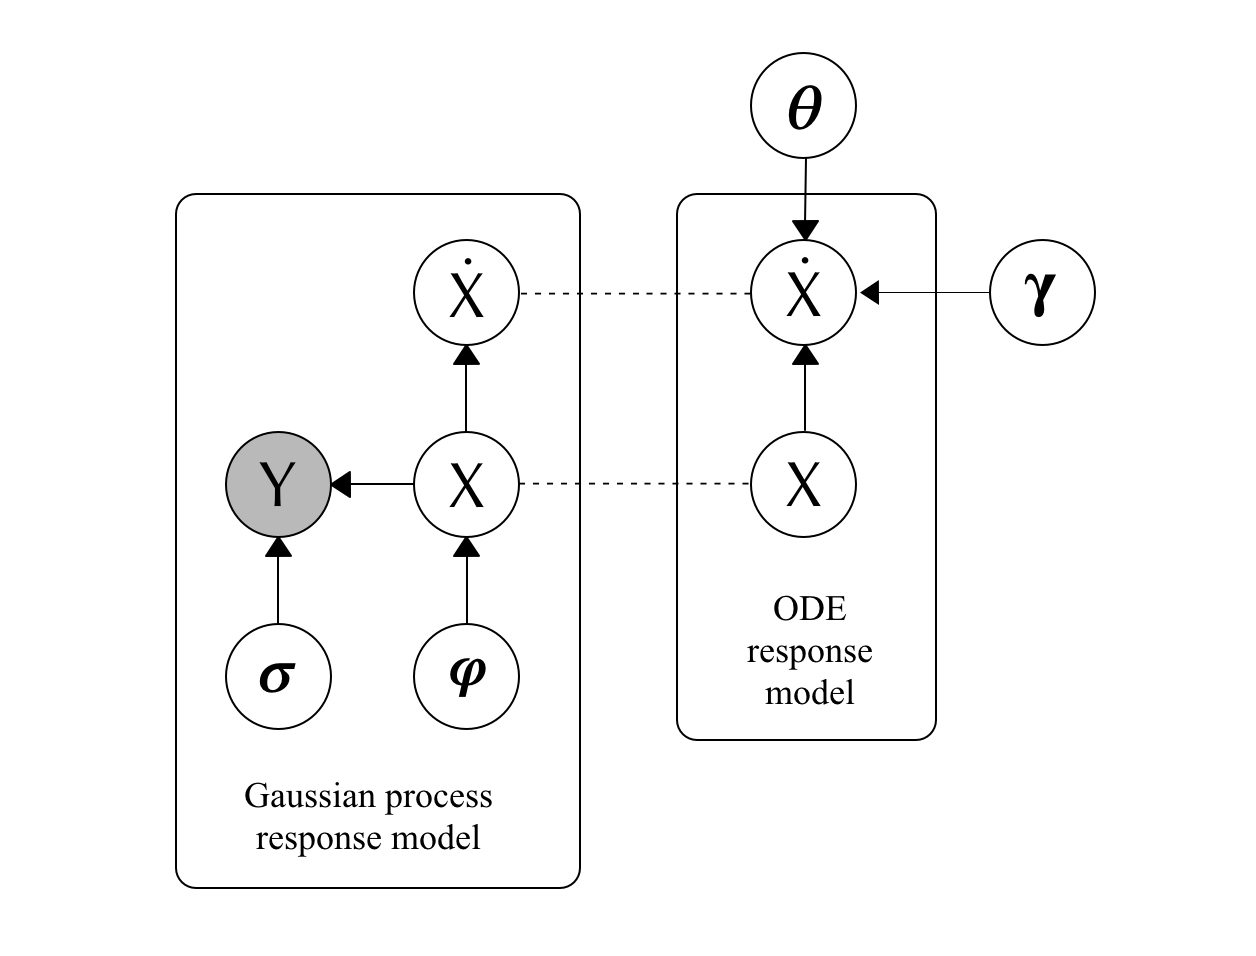
\includegraphics[width=0.8\textwidth]{graphics/gradient-matching-model}
    \caption{Graphical representation of the gradient matching with Gaussian processes model proposed by \cite{calderhead2009accelerating}. The dashed lines indicate information association from two response models using the product of experts \refequationp{\ref{eq-gmgp-poe}} . Details of the model are in \refsection{\ref{sec-sampling-gradient-matching}}.}    
    \label{fig-gmgp-model}
\end{figure}

\subsubsection*{Original sampling scheme}

\cite{calderhead2009accelerating} propose to integrate over the latent state derivatives $\dymdX$ to obtain
\begin{align}
    p(\dymtheta,\dymgamma\vert\dymX,\dymphi) 
    & =
    p(\dymtheta) p(\dymgamma) \int{
        p(\dymdX\vert\dymX,\dymtheta,\dymphi,\dymgamma)d\dymdX}
    \nonumber
    \\
    & \propto
    \frac{p(\dymtheta) p(\dymgamma)}{\mathcal{Z}(\dymgamma)} 
    \exp{[
        -\frac{1}{2}\sum_k{
            (\dymfkXshort{k} - \dymmk{k})^T\dymLambdak{k}(\dymfkXshort{k} - \dymmk{k})}]}
\end{align}
where $\dyminvLambdak{k} = \dymAk{k} + \dymgammak{k}\mI$, $\mathcal{Z}(\dymgamma) = \prod_k \lvert 2\pi(\dymAk{k} + \dymgammak{k}\mI) \rvert^{\frac{1}{2}}$ and $\dymfkXshort{k} = \dymfkX{k}$.

Then the sampling procedure follows the scheme below
\begin{align}
    \dymphi,\dymsigma 
    & \sim p(\dymphi,\dymsigma\vert\dymY)
    \label{eq-gmgp-sample-1}
    \\
    \dymX 
    & \sim p(\dymX\vert\dymY,\dymphi,\dymsigma)
    \label{eq-gmgp-sample-2}
    \\
    \dymtheta,\dymgamma 
    & \sim p(\dymtheta,\dymgamma\vert\dymX,\dymphi)
    \label{eq-gmgp-sample-3}    
\end{align}
where 
\begin{align}
    p(\dymphi, \dymsigma\vert\dymY) 
    & \propto p(\dymphi)p(\dymsigma)p(\dymY\vert\dymphi,\dymsigma) 
    \nonumber
    \\
    & \propto p(\dymphi)p(\dymsigma)\int{p(\dymX\vert\dymphi)p(\dymY\vert\dymX,\dymsigma)d\dymX}
    \nonumber
    \\
    & = p(\dymphi)p(\dymsigma)\prod_k{\mathcal{N}(\dymyk{k}\vert\mvector{0}, \dymCphik{k} + \dymsigmak{k}^2\mI)}    
    \nonumber
\end{align}

The sampling procedure requires two MCMC samplings for \refequationp{\ref{eq-gmgp-sample-1}} and \refequationp{\ref{eq-gmgp-sample-3}} respectively, and a direct sampling from the multivariate Gaussian distribution in \refequationp{\ref{eq-gmgp-sample-2}}.
The sampling steps are repeated until convergence is reached.

\subsubsection*{Adaptive sampling scheme}
One fundamental weakness of the previous sampling strategy is that the results on $\dymtheta$ and $\dymgamma$ from \refequationp{\ref{eq-gmgp-sample-3}} are never propagated back to \refequationp{\ref{eq-gmgp-sample-1}} and \refequationp{\ref{eq-gmgp-sample-2}}, and hence have no influence on the inference of states $\dymX$.
To close the feedback loop, \cite{dondelinger2013ode} proposed an improved sampling scheme called \emph{adaptive gradient matching}.

\cite{dondelinger2013ode} consider the joint distribution $p(\dymdX,\dymX,\dymphi,\dymtheta,\dymgamma)$, and show that its marginalization over the state derivatives $\dymdX$ is tractable:
\begin{align}
    p(\dymX,\dymphi,\dymtheta,\dymgamma)
    & = \int{
        p(\dymdX,\dymX,\dymphi,\dymtheta,\dymgamma) d\dymdX
        }
    \nonumber
    \\
    & = p(\dymX\vert\dymphi) p(\dymphi) p(\dymtheta) p(\dymgamma) \int{
        p(\dymdX\vert\dymX,\dymphi,\dymtheta,\dymgamma) d\dymdX}
    \nonumber
    \\
    & \propto \exp{[
        -\frac{1}{2}\sum_k{
            (\dymxk{k}^T\dyminvCphik{k}\dymxk{k} + (\dymfkXshort{k} - \dymmk{k})^T\dymLambdak{k}(\dymfkXshort{k} - \dymmk{k}))}]}
\end{align}

The full joint distribution, after integrating over the latent state derivatives $\dymdX$, is then given by
\begin{align}
    p(\dymY, \dymX, \dymphi, \dymtheta, \dymsigma, \dymgamma)
    & = p(\dymY\vert\dymX,\dymsigma) p(\dymX|\dymphi, \dymtheta, \dymgamma) p(\dymphi) p(\dymtheta) p(\dymsigma) p(\dymgamma)
    \nonumber
    \\
    & = p(\dymY\vert\dymX,\dymsigma) p(\dymX,\dymphi,\dymtheta,\dymgamma) p(\dymsigma)    
\end{align}

Based on the above joint distribution, \cite{dondelinger2013ode} devised an improved Metropolis-Hastings sampling scheme, which allows $\dymtheta$ to exert an influence on $\dymX$.

\subsubsection*{Summary}

To conclude this section, given the implicit solutions from the Gaussian processes, the states and parameters of the ODEs are inferred simultaneously without explicitly solving the ODEs anymore, which has led to significant speed-up.
Lastly, \cite{calderhead2009accelerating} also discuss the handling of partial observations, i.e.\ when some states are not observed, by utilizing to the prior we have imposed on the states \refequationp{\ref{eq-gmgp-x-prior}}.

\section{Variational gradient matching with Gaussian processes}
\label{sec-variational-gradient-matching}

Instead of using sampling methods, \cite{gorbach2016mean, gorbach2017scalable} proposed a solution to the previous problem based on variational inference, which has been shown, for specific types of ODEs \refequationp{\ref{eq-vgmgp-odes}} as discussed below, to be much more efficient than the sampling-based solutions, and scales well to large dynamical systems such the deterministic Lorenz 96 model with $1000$ states in their experiments.
This section gives an outline of the method by following the description from \cite{gorbach2017scalable} and the method is abbreviated as \algovgmgp\ in the rest of this work.

\subsubsection*{Maximum a posteriori estimation}

By combining the prior $p(\dymtheta)$, the state posterior  \refequationp{\ref{eq-gmgp-x-posterior}}, the product of experts result \refequationp{\ref{eq-gmgp-poe}}, and then integrating out the latent state derivatives $\dymdX$ as in \cite{calderhead2009accelerating}, the joint posterior $p(\dymX,\dymtheta\vert\dymY,\dymphi,\dymsigma,\dymgamma)$ is given as follows:
\begin{align}
    p(\dymX,\dymtheta\vert\dymY,\dymphi,\dymsigma,\dymgamma) 
    & = 
    p(\dymtheta)\int{
        p(\dymX\vert\dymY,\dymphi,\dymsigma) p(\dymdX\vert\dymX,\dymtheta,\dymphi,\dymgamma) d\dymdX
    }
    \nonumber
    \\
    & \propto
    p(\dymtheta) \prod_k{[
        \mathcal{N}(\dymxk{k}\vert\dymmuk{k}, \dymSigmak{k}) 
        \mathcal{N}(\dymfkX{k}\vert\dymmk{k},\dyminvLambdak{k})]}    
    \label{eq-vgmgp-posterior-joint}
\end{align}

Using the inference of the parameters $\dymtheta$ as an example, the ``best'' parameters $\dymtheta^*$ could ideally be estimated based on the \emph{maximum a posteriori (MAP)} of the posterior $p(\dymtheta\vert\dymY,\dymphi,\dymsigma,\dymgamma)$, which is equivalent to
\begin{align}
    \dymtheta^* = \argmax_{\dymtheta}\ln{p(\dymtheta\vert\dymY,\dymphi,\dymsigma,\dymgamma)}
    \label{eq-vgmgp-theta-posterior}
\end{align}
where the posterior on $\dymtheta$ is obtained by marginalizing \refequationp{\ref{eq-vgmgp-posterior-joint}} over the states $\dymX$, namely
\begin{align}
    p(\dymtheta\vert\dymY,\dymphi,\dymsigma,\dymgamma) = \int{p(\dymX,\dymtheta\vert\dymY,\dymphi,\dymsigma,\dymgamma)d\dymX}
    \nonumber
\end{align} 

However, the above equation is intractable due to strong non-linear couplings of the states induced by the ODEs \refequationp{\ref{eq-gmgp-odes}}.
As a workaround, \cite{gorbach2017scalable} designed a proxy distribution on the states and parameters denoted as $Q(\dymX, \dymtheta)$, and derived analytically tractable variational lower bounds based on mean-field variational inference.

\subsubsection*{Structural assumption}

First of all, the ODEs primarily considered by \cite{gorbach2017scalable} are state-wise of the following structure:
\begin{align}
    \dymfk{k} = \sum_m{\dymthetam{m}\prod_{i\in\mathcal{M}_{km}}{\dymxktn{i}{}}} + C
    \label{eq-vgmgp-odes}\
\end{align}
for $k = \mrange{1}{K}$, where $\mathcal{M}_{km}$ contains the states in the $k$-th equation of the ODEs that are controlled by the $m$-th parameter $\dymthetam{m}$, and $C$ denotes other terms that are independent of the parameters.
The first term of \refequationp{\ref{eq-vgmgp-odes}} can be viewed as a linear combination of the parameters and the product of the monomials of the states.
For the second term, the only requirement on terms in $C$ is that each state can only appear as monomial inside a term, but a term in $C$ can contain the product of the monomials of the states.

The structural assumption imposed on the ODEs leads to an important conclusion that the  following conditional distributions $p(\dymtheta\vert\dymY,\dymX,\dymphi,\dymgamma)$ and $p(\dymxk{u}\vert\dymY,\dymXwithoutk{u},\dymphi,\dymtheta,\dymsigma,\dymgamma)$ for $u = \mrange{1}{K}$ are Gaussian distributed, where $\dymXwithoutk{u} = \{\dymxk{o}\vert o = \mrange{1}{K}\ \text{and}\ o \neq u \}$, i.e.\ $\dymXwithoutk{u}$ is the set of all states except $\dymxk{u}$. 
But before writing out the distributions, we first need to introduce several more notations. 

One implication of the above assumption is that each ODE can be expressed as a linear combination of the parameters plus a term that is independent of them.
We therefore use $\dymBthetakX{k}$ and $\dymbthetakX{k}$ to denote the corresponding coefficients such that $\dymBthetakX{k}\dymtheta + \dymbthetakX{k} = \dymfkX{k}$ for $k = \mrange{1}{K}$.
Similarly, due to the monomial assumption about the states, each ODE can also be transformed into a linear combination of the $u$-th state for $u = \mrange{1}{K}$ plus an independent term.
Here we adopt the terms $\dymBukX{k}$ and $\dymbukX{k}$ to denote the respective coefficients such that $\dymBukX{k}\dymxk{u} + \dymbukX{k} = \dymfkX{k}$ for $k,u = \mrange{1}{k}$.

With these notations, we now state the conditional distributions $p(\dymtheta\vert\dymY,\dymX,\dymphi,\dymgamma)$ and $p(\dymxk{u}\vert\dymY,\dymXwithoutk{u},\dymphi,\dymtheta,\dymsigma,\dymgamma)$ as follows:
\begin{align}
    p(\dymtheta\vert\dymY,\dymX,\dymphi,\dymgamma)
    & = \mathcal{N}(\dymtheta\vert\dymrtheta, \dymOmegatheta)    
    \label{eq-vgmgp-theta-conditional}
    \\
    p(\dymxk{u}\vert\dymY,\dymXwithoutk{u},\dymphi,\dymtheta,\dymsigma,\dymgamma)
    & = \mathcal{N}(\dymxk{u}\vert\dymru, \dymOmegau)
    \label{eq-vgmgp-xu-conditional}
\end{align}
where 
\begin{align}
    \dymrtheta 
    & = \dymOmegatheta \sum_k{\dymBthetakX{k}^T\dymLambdak{k}(\dymmk{k} - \dymbthetakX{k})}    
    \label{eq-vgmgp-theta-conditional-mean}
    \\
    \dyminvOmegatheta
    & = \sum_k{\dymBthetakX{k}^T\dymLambdak{k}\dymBthetakX{k}}
    \label{eq-vgmgp-theta-conditional-covariance}
    \\
    \dymru
    & = \dymOmegau[
        \dyminvSigmak{u}\dymmuk{u}
        + \sum_k{
            \dymBukX{k}^T\dymLambdak{k}(\dymmk{k} - \dymbukX{k})}        
    ]
    \label{eq-vgmgp-xu-conditional-mean}
    \\
    \dyminvOmegau
    & = \dyminvSigmak{u} + \sum_k{
        \dymBukX{k}^T\dymLambdak{k}\dymBukX{k} 
    } 
    \label{eq-vgmgp-xu-conditional-covariance}
\end{align}
The proofs are omitted here and can be found in the supporting materials of \cite{gorbach2017scalable}.
They basically utilizes the formula to calculate the product of Gaussians \citep[\refsection{8.1}]{petersen2012matrix}, and the well-known closure property of Gaussian distribution under linear transformations, to obtain a closed-form solution.
As a side note, this conclusion will also be used later in \refchapter{\ref{ch-laplace-approximation}} to derive another approximate inference solution based on the Laplace approximation technique.

To simplify the notations, in the following, we will switch to the canonical form of \emph{exponential family} \citep[\refsection{9.2}]{murphy2012machine} to describe the distributions \refequationp{\ref{eq-vgmgp-theta-conditional}} and \refequationp{\ref{eq-vgmgp-xu-conditional}} as:
\begin{align}
    p(\dymtheta\vert\dymY,\dymX,\dymphi,\dymgamma)
    & = \dymhthetacanonical \exp{(\dymetathetacanonical^T\dymTthetacanonical - \dymAthetacanonical)}
    \label{eq-vgmgp-theta-conditional-canonical}
    \\
    p(\dymxk{u}\vert\dymY,\dymXwithoutk{u},\dymphi,\dymtheta,\dymsigma,\dymgamma)
    & = \dymhucanonical \exp{(\dymetaucanonical^T\dymTucanonical - \dymAucanonical)}
    \label{eq-vgmgp-xu-conditional-canonical}
\end{align}
where $\dymetacanonical, \dymTcanonical, \dymhcanonical, \dymAcanonical$ are the \emph{natural parameters}, \emph{sufficient statistics},  \emph{base measure} and \emph{log partition function} respectively .

\subsubsection*{Variational lower bound}

Introducing $\dymlambdavi$ and $\dympsiuvi$ for $u = \mrange{1}{K}$ as the variational parameters, the proxy distribution $Q(\dymX,\dymtheta)$ is constrained to the family $\mathcal{Q}$ that factorizes over the parameters and the states, and each factor is in the same exponential family as its corresponding counterparts defined in  \refequationp{\ref{eq-vgmgp-theta-conditional-canonical}} and \refequationp{\ref{eq-vgmgp-xu-conditional-canonical}} such that
\begin{align}
    \mathcal{Q} 
    & = \{
        Q(\dymX,\dymtheta)\vert Q(\dymX,\dymtheta) = q(\dymtheta\vert\dymlambdavi)\prod_u{q(\dymxk{u} \vert\dympsiuvi)}\}
    \label{eq-vgmgp-proxy-family}
    \intertext{where}
    q(\dymtheta\vert\dymlambdavi)
    & = \dymhthetacanonicalQ \exp{(
        \dymlambdavi^T\dymTthetacanonicalQ - \dymAthetacanonicalQ)}
    \nonumber
    \\
    q(\dymxk{u}\vert\dympsiuvi)
    & = \dymhucanonicalQ \exp{(
        \dympsiuvi^T\dymTucanonicalQ - \dymAucanonicalQ)}
    \nonumber
\end{align}

Using standard mean-field variation technique, the optimal $Q^*$ is given by
\begin{align}
    Q^* 
    & = \argmin_{Q(\dymX,\dymtheta)\in\mathcal{Q}}KL(Q(\dymX,\dymtheta)\|p(\dymX,\dymtheta\vert\dymY,\dymphi,\dymsigma,\dymgamma)) 
    \nonumber
    \\
    & = \argmax_{Q(\dymX,\dymtheta)\in\mathcal{Q}}\mathcal{L}_Q(\dymlambdavi,\dympsivi)
\end{align}
where $\mathcal{L}_Q(\dymlambdavi,\dympsivi)$ denotes the evidence lower bound.

\cite{gorbach2017scalable} showed that maximizing $\mathcal{L}_Q(\dymlambdavi,\dympsivi)$ with respect to $\dymtheta$ is equivalent to maximizing
\begin{align}
    \mathcal{L}_{\dymtheta}(\dymlambdavi) 
    & = \mathbb{E}_Q[
            \ln{p(\dymtheta\vert\dymY,\dymX,\dymphi,\dymgamma)}]
        - \mathbb{E}_Q[
            \ln{q(\dymtheta\vert\dymlambdavi)}]
    \nonumber             
    \\
    & = \mathbb{E}_Q[
        \dymetathetacanonical^T\nabla_{\dymlambdavi}\dymAthetacanonical] - \dymlambdavi^T\nabla_{\dymlambdavi}\dymAthetacanonicalQ
    \label{eq-vgmgp-elbo-theta}
\end{align}
and maximizing $\mathcal{L}_Q(\dymlambdavi,\dympsivi)$ with respect to $\dymxk{u}$ is equivalent to maximizing
\begin{align}
    \mathcal{L}_{\dympsiuvi} 
    & = \mathbb{E}_Q[
            \ln{p(\dymxk{u}\vert\dymY,\dymXwithoutk{u},\dymphi,\dymtheta,\dymsigma,\dymgamma)}]
        - \mathbb{E}_Q[
            \ln{q(\dymxk{u}\vert\dympsiuvi)}
        ]
    \nonumber
    \\
    & = \mathbb{E}_Q[
        \dymetaucanonical^T\nabla_{u}\dymAucanonical] -\dympsiuvi^T\nabla_{u}\dymAucanonicalQ
    \label{eq-vgmgp-elbo-xu}
\end{align}
where $\nabla_{(\cdot)}$ is the gradient operator.

Given the assumption about the conditional distributions \refequationp{\ref{eq-vgmgp-theta-conditional-canonical}} and \refequationp{\ref{eq-vgmgp-xu-conditional-canonical}}, plus the design of the proxy distribution family \refequationp{\ref{eq-vgmgp-proxy-family}}, they further showed that the lower bounds \refequationp{\ref{eq-vgmgp-elbo-theta}} and \refequationp{\ref{eq-vgmgp-elbo-xu}} can be optimized analytically by setting their gradients  with respect to their variational parameters to zero. 
The optimal variational parameters are thus given by
\begin{align}
    \dymlambdavi^*
    & = \mathbb{E}_Q[\dymetathetacanonical] 
    \label{eq-vgmgp-lambda-vi-optimal}
    \\
    \dympsiuvi^* 
    & = \mathbb{E}_Q[\dymetaucanonical]
    \label{eq-vgmgp-psiu-vi-optimal}
\end{align}
where the natural parameters are defined as $\dymetathetacanonical = [\dyminvOmegatheta\dymrtheta, -\frac{1}{2}\dyminvOmegatheta]^T$ and $\dymetaucanonical = [\dyminvOmegau \dymru, -\frac{1}{2}\dyminvOmegau]^T$.

\subsection*{\algovgmgp\ algorithm}

\begin{algorithm}
    \centering
    \caption{Pseudocode for the \algovgmgp\ algorithm.}
    \label{algo-vgmgp}
    \begin{algorithmic}[1]
        \For{$u = \mrange{1}{K}$}
            \State 
            \text{Initialize $\dymmuk{u}$, $\dymSigmak{u}$, $\dymmk{u}$ and $\dymLambdak{u}$ using Gaussian process regression}
        \EndFor
        \State
        \While{\text{not converged or maximum iteration not reached}}            
            \For{$u = \mrange{1}{K}$}
                \State 
                \text{Update the mean and variance of $\hat{q}_{\dympsiuvi}$ using $\mvector{\hat{\theta}}^{(i)}$}
            \EndFor                
            
            \State 
            \text{$\mvector{\hat{\theta}}^{(i+1)} = \argmax_{\dymtheta}{\mathbb{E}_Q[\sum_k{\ln{\mathcal{N}(\dymfkX{k}\vert\dymmk{k},\dyminvLambdak{k})}}]}$}
        \EndWhile
    \end{algorithmic}
\end{algorithm}

To close this section, the pseudocode of their algorithm is summarized in \refalgorithm{\ref{algo-vgmgp}}.
The algorithm first uses Gaussian process regression to obtain a smoothed estimate for the states and the distribution on the state derivatives.
As noted by \cite{gorbach2017scalable}, the Gaussian process priors come in naturally in cases where there exist unobserved states.

In the second step, the algorithm uses the variational gradient matching framework described before to maximize the lower bounds iteratively.
In every iteration, the states and parameters are optimized in an \emph{expectation-maximization (EM)} \cite[\refsection{9.4}]{bishop2006pattern} fashion until convergence is reached or the maximum allowed number of iterations is reached.




\begin{frame}[t]
    \frametitle{Laplace mean-field approximation}
    Positing the following factorized proxy distribution:
    \begin{align}
        Q(\dymX,\dymtheta) 
        & = 
        q(\dymtheta\vert\dymetatheta,\dymXitheta)
        \prod_u{
            q(\dymxk{u}\vert\dymetaxk{u},\dymXixk{u})}
        \nonumber
        \\
        & = \mathcal{N}(\dymtheta\vert\dymetatheta, \dymXitheta)
        \prod_u{
            \mathcal{N}(\dymxk{u}\vert\dymetaxk{u},\dymXixk{u})
        }
    \end{align}
\end{frame}

\begin{frame}[t]
    \frametitle{Conditional probability $p(\dymxk{u}\vert\dymY,\dymXwithoutk{u},\dymphi,\dymtheta,\dymsigma,\dymgamma)$}
    Denoting $\dymXwithoutk{u} = \{\dymxk{o}\vert o = \mrange{1}{K}\ \text{and}\ o \neq u \}$, for $u = \mrange{1}{K}$, we have
    \begin{align} 
        p(\dymxk{u}\vert\dymY,\dymXwithoutk{u},\dymphi,\dymtheta,\dymsigma,\dymgamma)       
        & =     
        \int{
            p(\dymxk{u}\vert\dymY,\dymXwithoutk{u},\dymphi,\dymsigma) p(\dymdX\vert\dymxk{u},\dymXwithoutk{u},\dymphi,\dymtheta,\dymgamma) d\dymdX}
        \nonumber
        \\
        & \stackrel{(b)}{=}         
        \int{
            p(\dymxk{u}\vert\dymyk{u},\dymphik{k},\dymsigmak{k}) p(\dymdX\vert\dymX,\dymphi,\dymtheta,\dymgamma) d\dymdX}
        \nonumber
        \\             
        & \propto
        \mathcal{N}(\dymxk{u}\vert\dymmuk{u},\dymSigmak{u})\prod_k{\mathcal{N}(\dymfkX{k}\vert\dymmk{k},\dyminvLambdak{k})}
        \label{eq-laplace-xu-objective}
    \end{align}
    where (b) holds because 
    \begin{itemize}
        \item[-] $p(\dymxk{u}\vert\dymY,\dymXwithoutk{u},\dymphi,\dymsigma)$ depends only on $\dymyk{u}$ due to independent prior assumption,
        \item[-] $p(\dymdX\vert\dymxk{u},\dymXwithoutk{u},\dymphi,\dymtheta,\dymgamma)$ is equivalent to $p(\dymdX\vert\dymX,\dymphi,\dymtheta,\dymgamma)$.
    \end{itemize}
\end{frame}

\begin{frame}[t]
    \frametitle{Cost minimization for states}
    The mean vector and precision matrix of $q(\dymxk{u}\vert\dymetaxk{u},\dymXixk{u})$ for $u = \mrange{1}{K}$ are given by
    \begin{align}
        \dymetaxk{u}
        & =     
        \argmax_{\dymxk{u}}{
            \ln{[
                \mathcal{N}(\dymxk{u}\vert\dymmuk{u},\dymSigmak{u})\prod_k{\mathcal{N}(\dymfkX{k}\vert\dymmk{k},\dyminvLambdak{k})}
            ]}
        }
        \nonumber
        \\
        & =     
        \argmax_{\dymxk{u}}{[
            \ln{\mathcal{N}(\dymxk{u}\vert\dymmuk{u},\dymSigmak{u})} 
            + \sum_k{
                \ln{\mathcal{N}(\dymfkX{k}\vert\dymmk{k},\dyminvLambdak{k})}
            }]}
        \nonumber
        \\
        & =
        \argmin_{\dymxk{u}}{
            \frac{1}{2}[(\dymxk{u} - \dymmuk{u})^T\dyminvSigmak{u}(\dymxk{u} - \dymmuk{u})
            + \sum_k{
                (\dymfkXshort{k} - \dymmk{k})^T\dymLambdak{k}(\dymfkXshort{k} - \dymmk{k})        
            }]
        }
        \nonumber
        \\
        & =
        \argmin_{\dymxk{u}}{
            cost_{\dymxk{u}}(\dymxk{u},\dymXwithoutk{u},\dymtheta,\dymmuk{u},\dymSigmak{u},\dymm,\dymLambda)
        }
        \label{eq-laplace-xu-cost}
        \\
        \dymXixk{u}^{-1} 
        & = 
        \nabla\nabla cost_{\dymxk{u}}\vert_{\dymxk{u} = \dymetaxk{u}}
        \label{eq-laplace-xu-covariance}
    \end{align}
\end{frame}

\begin{frame}[t]
    \frametitle{Conditional probability $p(\dymtheta\vert\dymY,\dymX,\dymphi,\dymgamma)$}
    For $p(\dymtheta\vert\dymY,\dymX,\dymphi,\dymgamma)$, we have
    \begin{align}
        p(\dymtheta\vert\dymY,\dymX,\dymphi,\dymgamma) 
        & \stackrel{(a)}{=} 
        p(\dymtheta\vert\dymX,\dymphi,\dymgamma) 
        \nonumber
        \\        
        & = 
        \int{
            p(\dymtheta) p(\dymdX\vert\dymX,\dymphi,\dymtheta,\dymgamma)d\dymdX}
        \nonumber
        \\               
        & \propto 
        \prod_k{\mathcal{N}(\dymfkX{k}\vert\dymmk{k},\dyminvLambdak{k})}
        \label{eq-laplace-theta-objective}
    \end{align}
    where $(a)$ holds since $\dymtheta$ depends indirectly on $\dymY$ through $\dymX$.
\end{frame}

\begin{frame}[t]
    \frametitle{Cost minimization for parameters}
    Denoting $\dymfkXshort{k} = \dymfkX{k}$, $\dymm = [\mrange{\dymmk{1}}{\dymmk{K}}]$, and $\dymLambda = [\mrange{\dymLambdak{1}}{\dymLambdak{K}}]$, then mean vector and precision matrix of $p(\dymtheta\vert\dymY,\dymX,\dymphi,\dymgamma)$ are given by
    \begin{align}
        \dymetatheta
        & = 
        \argmax_{\dymtheta}{
            \ln{
                \prod_k{\mathcal{N}(\dymfkX{k}\vert\dymmk{k},\dyminvLambdak{k})}
            }
        }
        \nonumber
        \\
        & = 
        \argmax_{\dymtheta}{
            \sum_k{
                \ln{\mathcal{N}(\dymfkX{k}\vert\dymmk{k},\dyminvLambdak{k})}
            }}
        \nonumber
        \\
        & =
        \argmin_{\dymtheta}{
            \frac{1}{2}\sum_k{
                (\dymfkXshort{k} - \dymmk{k})^T\dymLambdak{k}(\dymfkXshort{k} - \dymmk{k})
            }
        }
        \nonumber
        \\
        & = 
        \argmin_{\dymtheta}{
            cost_{\dymtheta}(\dymX,\dymtheta,\dymm,\dymLambda)
        }
        \label{eq-laplace-theta-cost}
        \\
        \dymXitheta^{-1} 
        & = 
        \nabla\nabla cost_{\dymtheta}\vert_{\dymtheta = \dymetatheta}  
        \label{eq-laplace-theta-covariance}    
    \end{align} 
\end{frame}

\begin{frame}[t]
    \frametitle{Inference algorithm}
    \begin{itemize}
        \item[-] Initialize using Gaussian process regression
        \item[-] Repeat until convergence or maximum iteration
        \begin{itemize}
            \item[-] Update $\dymtheta$ while keeping the others fixed
            \item[-] For $u = \mrange{1}{K}$, update $\dymxk{u}$ while keeping the others fixed
        \end{itemize}
        \item[-] Calculate precision matrices
    \end{itemize}    
\end{frame}

\begin{frame}[t]
    \frametitle{Derivation for the gradients and Hessians}
    Recall that $cost_{\dymxk{u}}$ for state $u$ is given by
    \begin{align}
        cost_{\dymxk{u}}
        =
            \frac{1}{2}[(\dymxk{u} - \dymmuk{u})^T\dyminvSigmak{u}(\dymxk{u} - \dymmuk{u})
            + \sum_k{
                (\dymfkXshort{k} - \dymmk{k})^T\dymLambdak{k}(\dymfkXshort{k} - \dymmk{k})        
            }]
        \nonumber
    \end{align}
    
    \vspace{\baselineskip}
    Using matrix derivative and the fact that $\dyminvSigmak{u}$ is symmetric, we have
    \begin{align}
        \nabla_{\dymxk{u}}\frac{1}{2}(\dymxk{u} - \dymmuk{u})^T\dyminvSigmak{u}(\dymxk{u} - \dymmuk{u}) 
        = \dyminvSigmak{u}\dymxk{u}
        \label{eq-laplace-mu-gradient}
        \\
        \nabla\nabla_{\dymxk{u}}\frac{1}{2}(\dymxk{u} - \dymmuk{u})^T\dyminvSigmak{u}(\dymxk{u} - \dymmuk{u}) 
        = \dyminvSigmak{u}
        \label{eq-laplace-mu-hessian}
    \end{align}    
\end{frame}

\begin{frame}[t]
    \frametitle{Derivation for the gradients and Hessians}
    Using \emph{chain rule} and the fact that $\dymLambdak{k}$ is symmetric, we have
    \begin{align}
        & \nabla_{\dymxk{u}}\frac{1}{2}(\dymfkXshort{k}-\dymmk{k})^T\dymLambdak{k}(\dymfkXshort{k}-\dymmk{k})
        \nonumber
        \\
        = &
        \begin{bmatrix}
            \frac{\partial(\dymfkXshort{k})_1}{\partial \dymxktn{u}{1}} 
            & 
            \cdots 
            & 
            \frac{\partial(\dymfkXshort{k})_N}{\partial \dymxktn{u}{1}}
            \\
            \vdots 
            &
            \ddots
            &
            \vdots
            \\
            \frac{\partial(\dymfkXshort{k})_1}{\partial \dymxktn{u}{N}} 
            &
            \cdots
            &
            \frac{\partial(\dymfkXshort{k})_N}{\partial \dymxktn{u}{N}} 
        \end{bmatrix}
        \dymLambdak{k}(\dymfkXshort{k}-\dymmk{k}) 
        \nonumber
        \\
        & -
        \begin{bmatrix}
            \frac{\partial(\dymmk{k})_1}{\partial \dymxktn{u}{1}} 
            & 
            \cdots 
            & 
            \frac{\partial(\dymmk{k})_N}{\partial \dymxktn{u}{1}}
            \\
            \vdots 
            &
            \ddots
            &
            \vdots
            \\
            \frac{\partial(\dymmk{k})_1}{\partial \dymxktn{u}{N}} 
            &
            \cdots
            &
            \frac{\partial(\dymmk{k})_N}{\partial \dymxktn{u}{N}} 
        \end{bmatrix}
        \dymLambdak{k}(\dymfkXshort{k}-\dymmk{k})  
    \end{align}
\end{frame}

\begin{frame}[t]
    \frametitle{Derivation for the gradients and Hessians}
    The $(i, j)$-th entry of the Hessian is given by
    \begin{align}
        &\frac{
            \partial^{2}\frac{1}{2}(\dymfkXshort{k}-\dymmk{k})^T\dymLambdak{k}(\dymfkXshort{k}-\dymmk{k})}{
            \partial\dymxktn{u}{i}\partial\dymxktn{u}{j}}
        \nonumber
        \\
        = & \begin{bmatrix}
            \frac{\partial^2(\dymfkXshort{k}-\dymmk{k})_1}{\partial\dymxktn{u}{i}\partial\dymxktn{u}{j}}
            &
            \cdots
            &
            \frac{\partial^2(\dymfkXshort{k}-\dymmk{k})_N}{\partial\dymxktn{u}{i}\partial\dymxktn{u}{j}}
        \end{bmatrix}
        \dymLambdak{k}(\dymfkXshort{k}-\dymmk{k}) 
        \nonumber
        \\
        & + 
        \begin{bmatrix}
            \frac{\partial(\dymfkXshort{k}-\dymmk{k})_1}{\partial\dymxktn{u}{j}}
            &
            \cdots
            &
            \frac{\partial(\dymfkXshort{k}-\dymmk{k})_N}{\partial\dymxktn{u}{j}}
        \end{bmatrix}
        \dymLambdak{k}
        \begin{bmatrix}
            \frac{\partial(\dymfkXshort{k}-\dymmk{k})_1}{\partial\dymxktn{u}{i}}
            \\
            \vdots
            \\
            \frac{\partial(\dymfkXshort{k}-\dymmk{k})_N}{\partial\dymxktn{u}{i}}
        \end{bmatrix}
    \end{align}
\end{frame}

\begin{frame}[t]
    \frametitle{Positivity constraint}
    Let
    \begin{align}
        \dymtheta = [\mrange{\dymthetam{1}}{\dymthetam{M}}]^\top = [\mrange{e^{\dymthetatildem{1}}}{e^{\dymthetatildem{M}}}]^\top        
    \end{align}
    
    Since the exponential function is monotonic, we can first find
    \begin{align}
        \dymthetatilde^* 
        & = 
        \argmin_{\dymthetatilde}{
            cost_{\dymtheta}(\dymX,e^{\dymthetatilde},\dymm,\dymLambda)
        }
        \nonumber
        \\
        & = 
        \argmin_{\dymthetatilde}{
            \sum_k{
                \ln{
                    \mathcal{N}(\mvector{f}_k(\mvector{X}, e^{\widetilde{\mvector{\theta}}}) \vert\dymmk{k},\dyminvLambdak{k}))}}}    
    \end{align}
    and then obtain $\dymtheta^*$ as
    \begin{align}
        \dymtheta^* = [\mrange{e^{\dymthetatildem{1}^*}}{e^{\dymthetatildem{M}^*}}]^\top
    \end{align}
    
    Since $e^r > 0$ for any $r \in \R$, we essentially restrict $\dymtheta^*$ to positive values.
\end{frame}

\begin{frame}[t]
    \frametitle{Positivity constraint}
    The positivity constraint on states can be achieved by transforming $cost_{\dymxk{u}}$ to $cost_{\dymxtildek{u}}$, where we define for $u = \mrange{1}{K}$
    \begin{align}
        \dymxk{u} = [\mrange{\dymxktn{u}{1}}{\dymxktn{u}{N}}]^\top = [\mrange{e^{\dymxtildexktn{u}{1}}}{e^{\dymxtildexktn{u}{N}}}]^\top
    \end{align}
    
    \vspace{\baselineskip}
    Using chain rule, we have for $u = \mrange{1}{K}$ and $n = \mrange{1}{N}$ the following:
    \begin{align}
        \frac{d\widetilde{x}_{u}(t_n)}{dt}
        & =
        \frac{d\ln{{x}_{u}(t_n)}}{dt}
        \nonumber
        \\
        & =
        \frac{1}{{x}_{u}(t_n)}\frac{d{x}_{u}(t_n)}{dt}
        \nonumber
        \\
        & =  
        \frac{
            f_{u}(
            e^{\mvector{\widetilde{x}}(t_n)}, \dymtheta)}{e^{\widetilde{x}(t_n)}}
    \end{align}
\end{frame}

\begin{frame}[t]
    \frametitle{Positivity constraint}
    Caveats
    \\
    \begin{itemize}
        \item[-] The covariance matrix for the new variables cannot be transformed back to the original variables easily.
        \item[-] Probabilistic interpretability is lost since proper change of random variables requires the evaluation of the Jacobian determinant, which is computationally expensive.
    \end{itemize}
\end{frame}
\chapter{Extension to Random Dynamical Systems}
\label{ch-rodes}

As another important family of differential equations, \emph{random ordinary differential equations (RODEs)} are closely related to both ODEs and SDEs.
A system of RODEs is simply a set of ODEs with a stochastic process in its vector field functions \citep{kloeden2007pathwise}, while an SDE system can be analyzed using its RODE counterpart \citep{sussmann1978gap, imkeller2001conjugacy}.
Since RODEs are pathwise ODEs, the Laplace mean-field approximation described in \refchapter{\ref{ch-laplace-approximation}} can then be used to infer the states and parameters of the RODEs, or equivalently, the corresponding SDEs.

This chapter is organized as follows.
\refsection{\ref{sec-rodes}} gives a brief introduction to RODEs.
In \refsection{\ref{sec-rodes-laplace}}, the Laplace mean-field approximation technique is applied to RODEs to devise an \emph{ensemble}-like \citep[\refsection{16.6}]{murphy2012machine} solution to infer the states and parameters for diffusion processes.
We demonstrate the performance and accuracy of the solution empirically by comparing with other state-of-art techniques in \refchapter{\ref{ch-experiments}}.

\section{Random ordinary differential equations}
\label{sec-rodes}

Adopting the definition from \cite{kloeden2007pathwise}, RODEs are simply ODEs with a stochastic process in their vector fields.
Let $\mvector{f}: \R^K\times\R^W\mapsto\R^K$ be a continuous function, and $(\mvector{\zeta}_t)_{t\in [0,T]}$ be an $\R^W$ valued stochastic process with continuous sample paths defined on the complete probability space $\probspace$.  
For all $\mvector{\omega} \in \mvector{\Omega}$, a $K$-dimensional RODE defined as
\begin{align}
    \frac{d\dymx}{dt} = \mvector{f}(\dymx, \mvector{\zeta}_t(\mvector{\omega}))
    \label{eq-rodes}
\end{align}
is a \emph{non-autonomous} ODE system
\begin{align}
    \dymdx = \frac{d\dymx}{dt} = \mvector{F}_{\mvector{\omega}}(\mvector{x}, t) = \mvector{f}(\dymx, \mvector{\omega}_t)
    \label{eq-rodes-odes}
\end{align}
An example \citep{grune2001pathwise} of a scalar RODE with additive noise is given by
\begin{align}
    \frac{dx(t)}{dt} = -x + \cos{(W_t(\omega))}
    \label{eq-rodes-example}
\end{align}
where $W_t$ is a one-dimensional Wiener process.
A RODE example with multiplicative noise can be defined similarly but is not considered in this work.

Following \cite{kloeden2007pathwise}, to ensure the existence of a unique solution for the initial value problem defined in \refsection{\ref{sec-odes}} on the finite time interval $[0,T]$, we typically assume that $\mvector{f}$ is arbitrarily smooth, i.e.\ it is infinitely differentiable in its variables, and thus is locally \emph{Lipschitz} in $\mvector{x}$. 
Since the stochastic process is usually only \emph{H{\"o}lder continuous} in time, the vector fields of the non-autonomous ODEs $\mvector{F}_{\mvector{\omega}}(\mvector{x}, t)$ are therefore continuous but not differentiable in time for every fixed realization of $\mvector{\omega} \in \mvector{\Omega}$.

Because for every fixed realization of $\mvector{\omega} \in \mvector{\Omega}$, the RODEs \refequationp{\ref{eq-rodes}} turn into a deterministic ODE system \refequationp{\ref{eq-rodes-odes}}, one approach to solving the RODEs is to use sampling methods to first obtain many sample paths, and then solving each sample path deterministically.
In order to cover the statistics of the solution, a massive number of ODEs must be solved efficiently.
A high performance related study was conducted by \cite{riesinger2016solving}, where the sample paths are solved in parallel on a modern GPU cluster.

\section{Doss-Sussmann/Imkeller-Schmalfuss correspondence}
\label{sec-doss-sussmann}

Since a system of RODEs can be analyzed pathwise using deterministic calculus, it offers an opportunity to study its related SDEs as discussed below.

First of all, it has been shown by \cite{jentzen2011taylor} that any RODE system with a Wiener process can be expressed as its equivalent SDE system. 
Using the scalar RODE in \refequationp{\ref{eq-rodes-example}} as an example, its SDE formulation is described as
\begin{align}
    d\begin{pmatrix}
        x_t 
        \\ 
        y_t
    \end{pmatrix}
    & = 
    \begin{pmatrix}
        -x_t + \cos{(y_t)}
        \\
        0
    \end{pmatrix}
    + 
    \begin{pmatrix}
        0
        \\
        1
    \end{pmatrix}
    dW_t
\end{align}

Similarly, any finite dimensional SDE system can be transformed into its equivalent ODEs by utilizing the \emph{Doss-Sussmann/Imkeller-Schalfuss correspondence} \citep{sussmann1978gap, imkeller2001conjugacy}.
Specifically, for SDE models with additive noise, the statement from \cite[\refchapter{2}]{jentzen2011taylor} is stated as the following proposition.
\begin{proposition}
    Any finite dimensional SDE system can be transformed into an equivalent RODE system and vice versa as follows:
    \begin{align}
        \sdedx = \sdef\sdedt + \sdedwt 
        \iff 
        \frac{\rodedz}{dt} = \rodef + \rodeo
        \label{eq-rode-sde}
    \end{align}
    where $\rodez = \sdex - \rodeo$ and $\rodeo$ is a stationary stochastic \emph{Ornstein-Uhlenbeck} process defined as
    \begin{align}
        d\rodeo = -\rodeo\sdedt + \sdedwt
    \end{align}
\end{proposition}  

\section{Laplace mean-field for random dynamical systems}
\label{sec-rodes-laplace}

As discussed previously, although RODE sample paths can be analyzed using deterministic calculus, the existence of the stochastic process causes traditional numerical schemes such as the \emph{Euler} and the \emph{Runge-Kutta} methods \citep{butcher2016numerical} to fail to achieve their usual order of convergence when applied to RODEs \citep{grune2001pathwise}.
In the past, improved numerical solutions such as the integral versions of the implicit Taylor-like expansions \citep{kloeden2007pathwise} have been proposed to achieve better result.

On the other hand, since the solution paths of the RODEs are once differentiable, the gradient matching model can be ideally applied to the RODEs.
Moreover, the computational efficiency of the \algolpmf\ method allows a large number of RODE sample paths to be solved simultaneously. 
Lastly, by using the Doss-Sussmann/Imkeller-Schalfuss correspondence described before, we derive the following ensemble gradient matching algorithm, denoted as \algolpmfsde, to infer the states and the parameters of the SDEs without requiring any stochastic calculus.

\begin{algorithm}
    \centering
    \caption{Pseudocode for the \algolpmfsde\ algorithm.}
    \label{algo-lpmf-sde}
    \begin{algorithmic}[1]
        \State{Transform the SDEs into RODEs using \refequationp{\ref{eq-rode-sde}}.}
        \State{Generate $N_{paths}$ RODEs sample paths using each time an independently generated Ornstein-Uhlenbeck process sample path.}
        \For{$i = \mrange{1}{N_{paths}}$}
            \State{Estimate the states and parameters using \refalgorithm{\ref{algo-lpmf}}.}
        \EndFor
        \State{Average the estimation results from all the sample paths.}
    \end{algorithmic}
\end{algorithm}

Since the experiments are conducted with the Lorenz 63 and the Lorenz 96 models, the estimation of the parameters are carried out by extending the closed-forms solutions from \refequationp{\ref{eq-vgmgp-theta-conditional-mean}} and \refequationp{\ref{eq-vgmgp-theta-conditional-covariance}} as follows:
\begin{align}
    \dymetatheta 
    & = \dymOmegatheta \sum_k{\dymBthetakX{k}^T\dymLambdak{k}(\dymmk{k} - \dymbthetakX{k} - \mdata{O}_k)}    
    \\
    \dymXitheta^{-1}
    & = \sum_k{\dymBthetakX{k}^T\dymLambdak{k}\dymBthetakX{k}}
\end{align}
where 
\begin{align}
    \dymmk{k} &= \dymdCdphik{k}\dyminvCphik{k}\mvector{z}_k
    \\
    \dyminvLambdak{k} &= \dymdCdphik{k} - \dymdCphik{k}\dyminvCphik{k}\dymCdphik{k} + \dymgamma_k \mvector{I}
\end{align}
Similar to the notations introduced in \refsection{\ref{sec-odes}}, $\mvector{z}_u \in \R^N$ and $\mdata{Z} \in \R^{K \times N}$ refer to the states of the RODE sample path, while $\mdata{O}$ refer to the states of the Ornstein-Uhlenbeck process.
Note that the rewriting of the vector field as a linear combination of the parameters $\dymtheta$ and an extra term should satisfy
\begin{align}
    \mvector{B}_{\dymtheta k}(\mdata{Z} + \mvector{O})\dymtheta + \mvector{b}_{\dymtheta k}(\mdata{Z} + \mdata{O}) + \mdata{O} 
    = 
    \mvector{f}_k(\mdata{Z} + \mdata{O}, \dymtheta) + \mdata{O}
\end{align}
for $k = \mrange{1}{K}$.

Due to the complexity of expressing as a linear combination of the states and an extra term, the states of the RODE sample path are estimated using gradient-descent by minimizing the adapted cost function \refequationp{\ref{eq-laplace-xu-cost}} as follows:
\begin{align}
    cost_{\mvector{z}_u} 
    &= \ln{[\mathcal{N}(\mvector{z}_u\vert\mvector{\mu}(\mvector{y}_u), \dymSigmak{u})\prod_k{
        \mathcal{N}(\mvector{f}_k(\mdata{Z} + \mdata{O}, \dymtheta) + \mdata{O}\vert\dymmk{k},\dyminvLambdak{k}))]}
    }
\end{align}
for $u = \mrange{1}{K}$,  where
\begin{align}
    \dymmuk{u} &= \dymCphik{u}(\dymCphik{u} + \dymsigmak{u}^2\mI)^{-1}\dymyk{u}
    \\
    \dymSigmak{u} &= \dymsigmak{u}^2\dymCphik{u}(\dymCphik{u} + \dymsigmak{u}^2\mI)^{-1}
\end{align}

\chapter{Experiments}
\label{ch-experiments}

This chapter examines the estimation accuracy, runtime performance and scalability of the general \algolpmf\ method and its extensions introduced in \refchapter{\ref{ch-laplace-approximation}} and \refchapter{\ref{ch-rodes}} by comparing with the other state-of-art inference techniques empirically.
In \refsection{\ref{sec-implementation}}, the implementation of the algorithms is discussed.
Then four dynamical systems with different dimensionality and complexity are used for the experiments.
\refsection{\ref{sec-lotka-volterra}} and \refsection{\ref{sec-protein-signalling-transduction-pathway}} consider the state and parameter estimation for deterministic dynamical systems, while \refsection{\ref{sec-lorenz-96}} and \refsection{\ref{sec-lorenz-63}} consider two random dynamical systems.

\section{Implementation}
\label{sec-implementation}

The source code of this work is implemented from the ground up using the general purpose programming language Python 3\footnote{\url{https://www.python.org/}}.
The MATLAB\footnote{\url{https://www.mathworks.com/products/matlab.html}} code for the \algovgmgp\ algorithm from \cite{gorbach2017scalable} is used as the blueprint during implementation.
Several important open-source packages have made this Python solution possible:
\begin{itemize}
    \item The SciPy\footnote{\url{https://www.scipy.org/}} package provides a powerful optimization module and other I/O utilities to read and write files in MATLAB format.
    \item The NumPy\footnote{\url{http://www.numpy.org/}} package is the backbone for linear algebra operations and random variable generation.
    \item The SymPy\footnote{\url{http://www.sympy.org/en/index.html}} package is used for symbolic mathematics when implementing the general interface for dynamical systems and kernel functions. It is also used to calculate the gradients and Hessians of the cost functions for part of the solution.
    \item The matplotlib\footnote{\url{http://matplotlib.org/}} package helps to produce publication quality plotting.
    \item The Jupyter Notebook\footnote{\url{http://jupyter.org/}} is used as the GUI interface to combine code, visualizations and documentation in a sharable format.
    \item The sdeint\footnote{\url{https://github.com/mattja/sdeint}} package provides the numerical methods to solve SDEs. 
    \item The TensorFlow\footnote{\url{https://www.tensorflow.org/}} package is a machine learning library popular among the deep learning community, which provides auto-differentiation support for part of the solution.
\end{itemize}


\section{Lotka-Volterra model}
\label{sec-lotka-volterra}

The first deterministic dynamical system examined in this chapter is the \emph{Lotka-Volterra} model \citep{lotka1932growth}, which is frequently used in ecology to describe the interaction between the prey species and the predator species over time.
The model consists of two first-order, nonlinear differential equations where the states $x(t), y(t)\in \R_{\geqslant 0}$ are the populations of the prey and the predator respectively at time point $t$.
The ODEs of the model are given by
\begin{align}
    \dot{x}(t) & = \alpha x(t) - \beta x(t)y(t)
    \nonumber
    \\
    \dot{y}(t) & = \delta x(t)y(t) - \gamma y(t)
    \label{eq-lotka-odes}
\end{align}
where $\alpha, \beta, \delta, \gamma \in \R^+$ are the parameters controlling the dynamics.
 

\subsubsection*{Experimental setup}

\begin{table}
\centering
\caption{Experimental setup for the Lotka-Volterra model. The system dimension is denoted by $K$ and the number of observable dimensions is $K_{obs}$. Based on the parameter values $\alpha$, $\beta$, $\delta$, and $\gamma$, the ODEs are integrated from time $t_0$ to $t_T$ with a step size of $\delta t$. The observation noise variance $\dymsigmak{k}^2$ is assumed to be the identical for each state. For each time unit, $freq_{obs}$ denotes the number of observations to be collected, which are equally distributed over the time line.}
\label{table-lotka-setup}
\begin{tabular}{|c|c|c|c|c|c|c|c|c|}
\hline
$K$ & $K_{obs}$ & $t_0$ & $t_T$ & $\delta t$ & $\alpha, \beta, \delta, \gamma$ & $\dymsigmak{k}^2$  & $freq_{obs}$ \\ \hline
2 & 2 & 0 & 2 & 0.01 & 2, 1, 1, 4 & 0.1 & 10 \\ \hline
\end{tabular}
\end{table}

\reftable{\ref{table-lotka-setup}} shows the setup for the experiment.
The experiment is repeated 10 times with each time an independently collected observation set.
Since the \algolpmf\ method is derived from the \algovgmgp\ method, in the following, we compare the results using both methods.
The \algolpmf\ method is run first without any positivity constraint and then it is run again with positivity constraint on the parameters, which are referred to as \algolpmf\ and \algolpmfpos\ respectively.
It would be interesting to constrain both the states and the parameters to be positive, but the inference fails as shown in \reffigure{\ref{fig-lotka-fail}}. 
The reason for that in unclear yet due to time constraints and requires further investigation.
In order to provide a fair comparison in terms of runtime, both methods are deployed on a desktop with an Intel i5 quad-core CPU and 16 GB of memory.

\begin{figure}
    \centering
    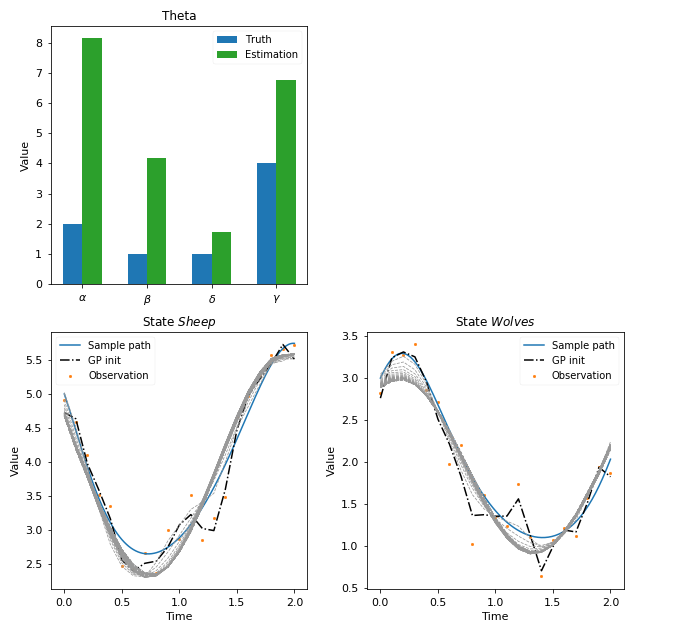
\includegraphics[width=0.8\textwidth]{graphics/lotka-fail}
    \caption{Inference for the Lotka-Volterra model fails when both the states and parameters are constrained to be positive.}
    \label{fig-lotka-fail}
\end{figure}

\subsubsection*{State estimation}

\begin{figure}
    \centering
    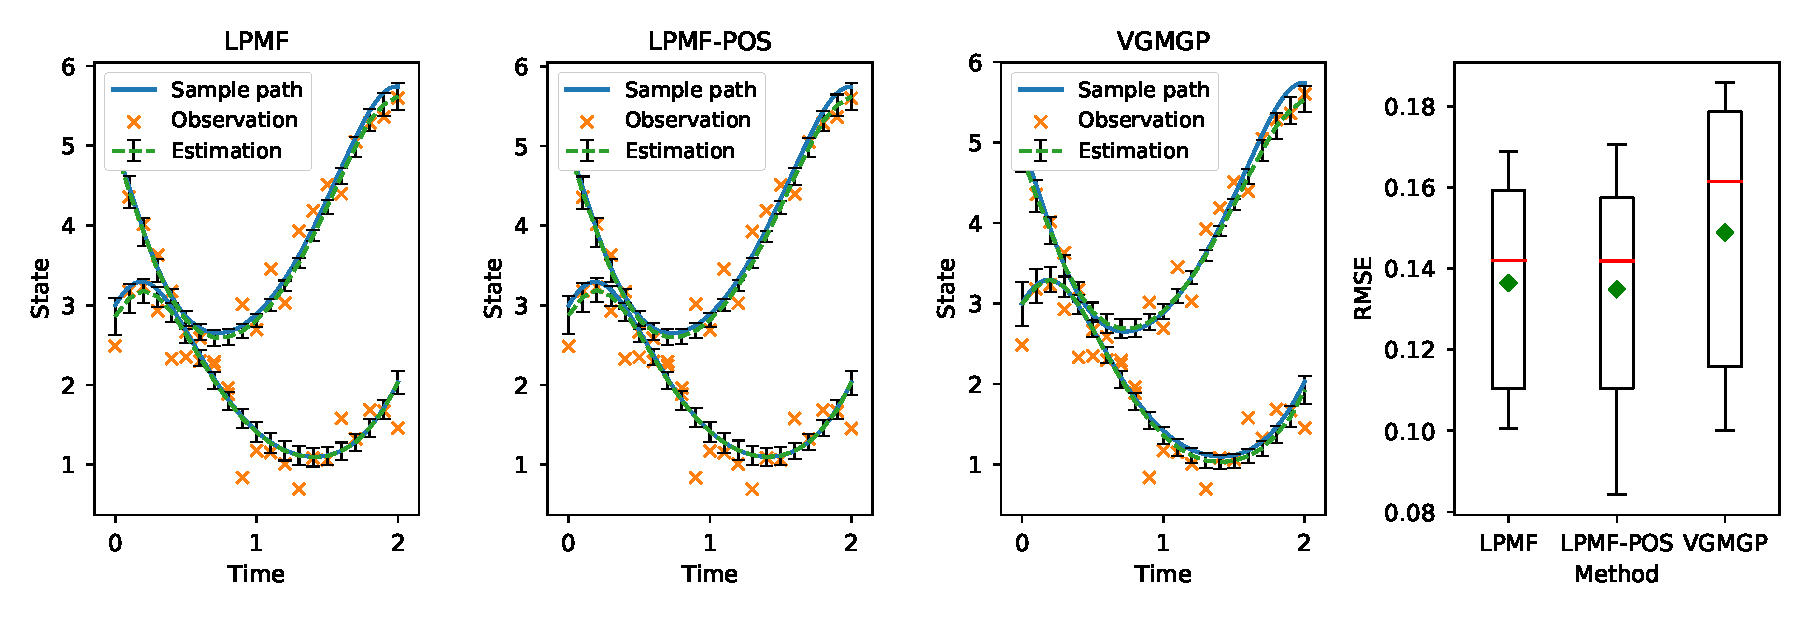
\includegraphics[width=\textwidth]{graphics/lotka-states}
    \caption{State estimation results for the Lotka-Volterra model. The left plot shows the result using \algolpmf; the left middle plot shows the result using \algolpmfpos; the right middle plot shows the result using \algovgmgp; the right plot summarizes the RMSE after 10 independent runs. The error bars in the first three plots indicate one standard deviation.}
    \label{fig-lotka-state}
\end{figure}

\reffigure{\ref{fig-lotka-state}} shows the results after the 10 independent runs.
For illustration purposes, the observations from one run is also plotted to indicate the noise level.
The dotted green lines are obtained by averaging the means of the state estimation for the 10 runs, while the error bars indicate one standard deviation of the means.
The figure shows that the state estimation results are very close to each other and is almost identical to the ground truth.

To quantify the accuracy, the root mean square error (RMSE) is used and is defined as follows:
\begin{align}
    RMSE
    & = \frac{1}{K}\sum_{k}{\sqrt{
        \frac{1}{N}\sum_{n=1}^N{
            (\dymxhatktn{k}{n} - \dymxktn{k}{n})^2
        }
    }}    
\end{align}
where $K$ indicates the number of states, $N$ is the total number of observations for each dimension, and $\dymxhatktn{k}{n}$ and $\dymxktn{k}{n}$ are the predicted and true values for the $k$-th state at time point $t$ respectively.
The RMSEs are very close to each other with the \algolpmf\ method having slightly lower error.

\subsubsection*{Parameter estimation}

\begin{figure}
    \centering
    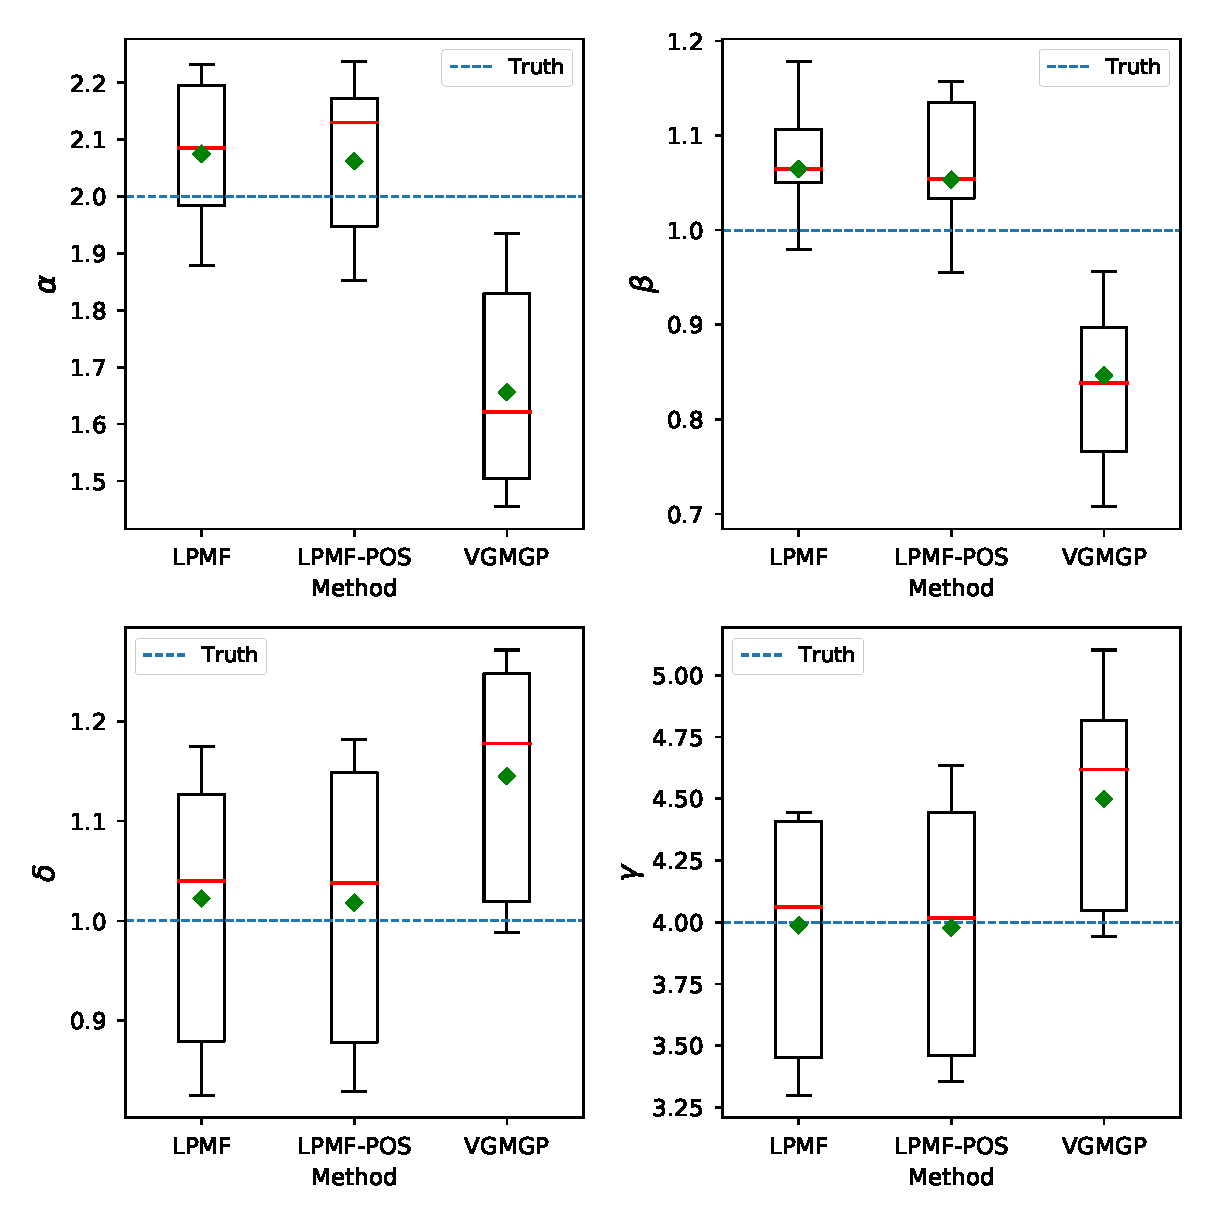
\includegraphics[width=1\textwidth]{graphics/lotka-parameters-boxplot}
    \caption{Parameter estimation results for the Lotka-Volterra model. In the box plot, the median is indicated by the red line, while the mean is shown as the green diamond. The box shows the lower and upper quartiles, while the whiskers are the 5th and 95th percentiles. The true parameter value is shown as the dotted blue line.}
    \label{fig-lotka-parameters-boxplot}
\end{figure}

The estimation results for the parameters of the Lotka-Volterra model are shown in \reffigure{\ref{fig-lotka-parameters-boxplot}}.
The \algolpmf\ method again achieves better results than the \algovgmgp\ algorithm, even with the positivity constraint on the parameters.
The mean values for the prediction from \algolpmf\ are also very close to the true parameter values.

To explain this, first note that both methods assume the decoupling of states from the other states and the decoupling of the states and the parameters when constructing the proxy distribution $Q$.
However, the \algovgmgp\ method further assumes the decoupling of the same states across time points, which is not the case for \algolpmf.
Since the ODEs of the Lotka-Volterra model satisfies the structural assumption, if the conditional distributions in \refequationp{\ref{eq-vgmgp-theta-conditional}} and \refequationp{\ref{eq-vgmgp-xu-conditional}} are indeed Gaussian, then Laplace approximation is expected to correctly find the mode the distribution.

\subsubsection*{Runtime performance}

\begin{figure}
    \centering
    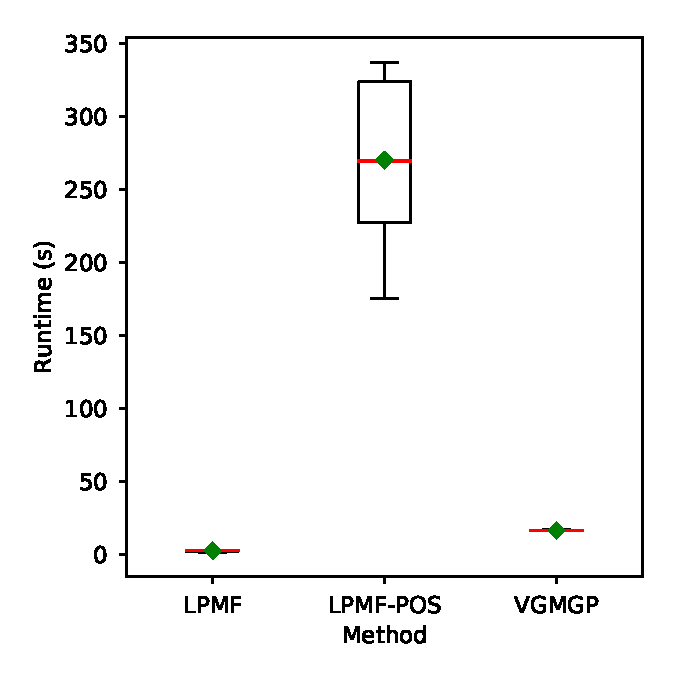
\includegraphics[width=0.48\textwidth]{graphics/lotka-runtime-boxplot}
    \caption{Runtime performance for the Lotka-Volterra model. In the box plot, the median is indicated by the red line, while the mean is shown as the green diamond. The box shows the lower and upper quartiles, while the whiskers are the 5th and 95th percentiles.}
    \label{fig-lotka-runtime-boxplot}
\end{figure}

In terms of runtime, both the \algolpmf\ method when no positivity constraint is imposed and the \algovgmgp\ method are extremely fast.
On average, the \algolpmf\ method finishes in 2.4 seconds and the \algovgmgp\ method completes in 16.3 seconds.
Since \algolpmf\ is implemented in Python while \algovgmgp\ is implemented MATLAB, exact comparison is infeasible.
In general, the \algolpmf\ is likely to be more efficient since the evaluation of the expectations \refequationp{\ref{eq-vgmgp-lambda-vi-optimal}} and \refequationp{\ref{eq-vgmgp-psiu-vi-optimal}} is not required.
Moreover, the states is inferred by minimizing the cost function for the \algolpmf\ method in this experiment.
If closed-form solutions are used, it would be expected to even faster.

Lastly, it is unclear what causes the slow down of the \algolpmf\  algorithm after the introduction of the positivity constraint.
Given the time constraints and in order to achieve fast prototyping, the gradients and Hessians of the cost functions with positivity constraints are obtained from symbolic libraries.
This is in contrast to the highly vectorized implementation when no positivity constraint is enforced.
Part of the reason is probably due to the inefficient implementation, but it requires further investigation.

\section{Protein signalling transduction pathway}
\label{sec-protein-signalling-transduction-pathway}

As already mentioned in \refsection{\ref{sec-motivation}}, the biochemical \emph{protein signalling transduction pathway} \citep{vyshemirsky2007bayesian} is a signal transduction cascade model describing the dynamics among protein species.
The model can be represented by the following 5-dimensional ODEs:
\begin{align}
    \proteinSdt 
    & = 
    -\proteinki{1} \times \proteinS 
    -\proteinki{2} \times \proteinS \times \proteinR
    + \proteinki{3} \times \proteinRS
    \nonumber
    \\
    \proteindSdt
    & = 
    \proteinki{1} \times \proteinS    
    \nonumber
    \\
    \proteinRdt
    & =
    -\proteinki{2} \times \proteinS \times \proteinR 
    + \proteinki{3} \times \proteinRS
    + \proteinV \times \frac{\proteinRpp}{\proteinKm + \proteinRpp}
    \nonumber
    \\
    \proteinRSdt
    & =
    \proteinki{2} \times \proteinS \times \proteinR
    - \proteinki{3} \times \proteinRS
    - \proteinki{4} \times \proteinRS
    \nonumber
    \\
    \proteinRppdt 
    & =
    \proteinki{4} \times \proteinRS - \proteinV \times \frac{\proteinRpp}{\proteinKm + \proteinRpp}
\end{align}
where the input signal is the concentration level of the protein $\proteinS$, which can either bind to the protein $\proteinR$ to form the complex $\proteinRS$, or activate it into its phosphorylated form $\proteinRpp$, or degrade into $\proteindS$.
The protein $\proteinRpp$ can be deactivated.
The conversion between $\proteinRpp$ and $\proteinR$ is governed by the \emph{Michaelis-Menten kinetic law} with parameters $\proteinV$ and $\proteinKm$, while the rest of the interactions are defined by the \emph{Mass Action kinetic law} with their respective parameters $\proteinki{1}, \proteinki{2}, \proteinki{3}$ and $\proteinki{4}$.

Different from other dynamical models in this chapter, the state $Rpp$ and the parameter $K_m$ both violate the structural assumption on the ODEs.
It is also a difficult benchmark system due to the large number of parameters and its sensitivity to noise.
In this section, we use the \algolpmf\ method with positivity constraint on the parameters to run the experiment.

\reftable{\ref{table-protein-setup}} shows the experimental setup. 
Since the states flattens out towards the end, the observation time points are set to 0, 1, 2, 4, 5, 7, 10, 15, 20, 30, 40, 50, 60, 80 and 100.
Because the observations in this experiment are required to be positive, when the noise is too big to generate negative observations, it is resampled until the positivity requirement is satisfied.

\begin{table}
\centering
\caption{Experimental setup for the protein signaling transduction pathway model. The system dimension is denoted by $K$ and the number of observable dimensions is $K_{obs}$. Based on the parameters $k_1, k_2, k_3, k_4, V, Km$, the ODEs are solved from time $t_0$ to $t_T$ with a step size of $\delta t$. The observation noise variance $\dymsigmak{k}^2$ is assumed to be the identical for each state.}
\label{table-protein-setup}
\begin{tabular}{|c|c|c|c|c|c|c|c|c|}
\hline
$K$ & $K_{obs}$ & $t_0$ & $t_T$ & $\delta t$ & $k_1, k_2, k_3, k_4, V, Km$ & $\dymsigmak{k}^2$ \\ \hline
5 & 5 & 0 & 100 & 0.05 & 0.07, 0.6, 0.05, 0.3, 0.017, 3 & 0.01\\ \hline
\end{tabular}
\end{table}

\subsubsection*{Direct inference on $Rpp$}

\begin{figure}
    \centering
    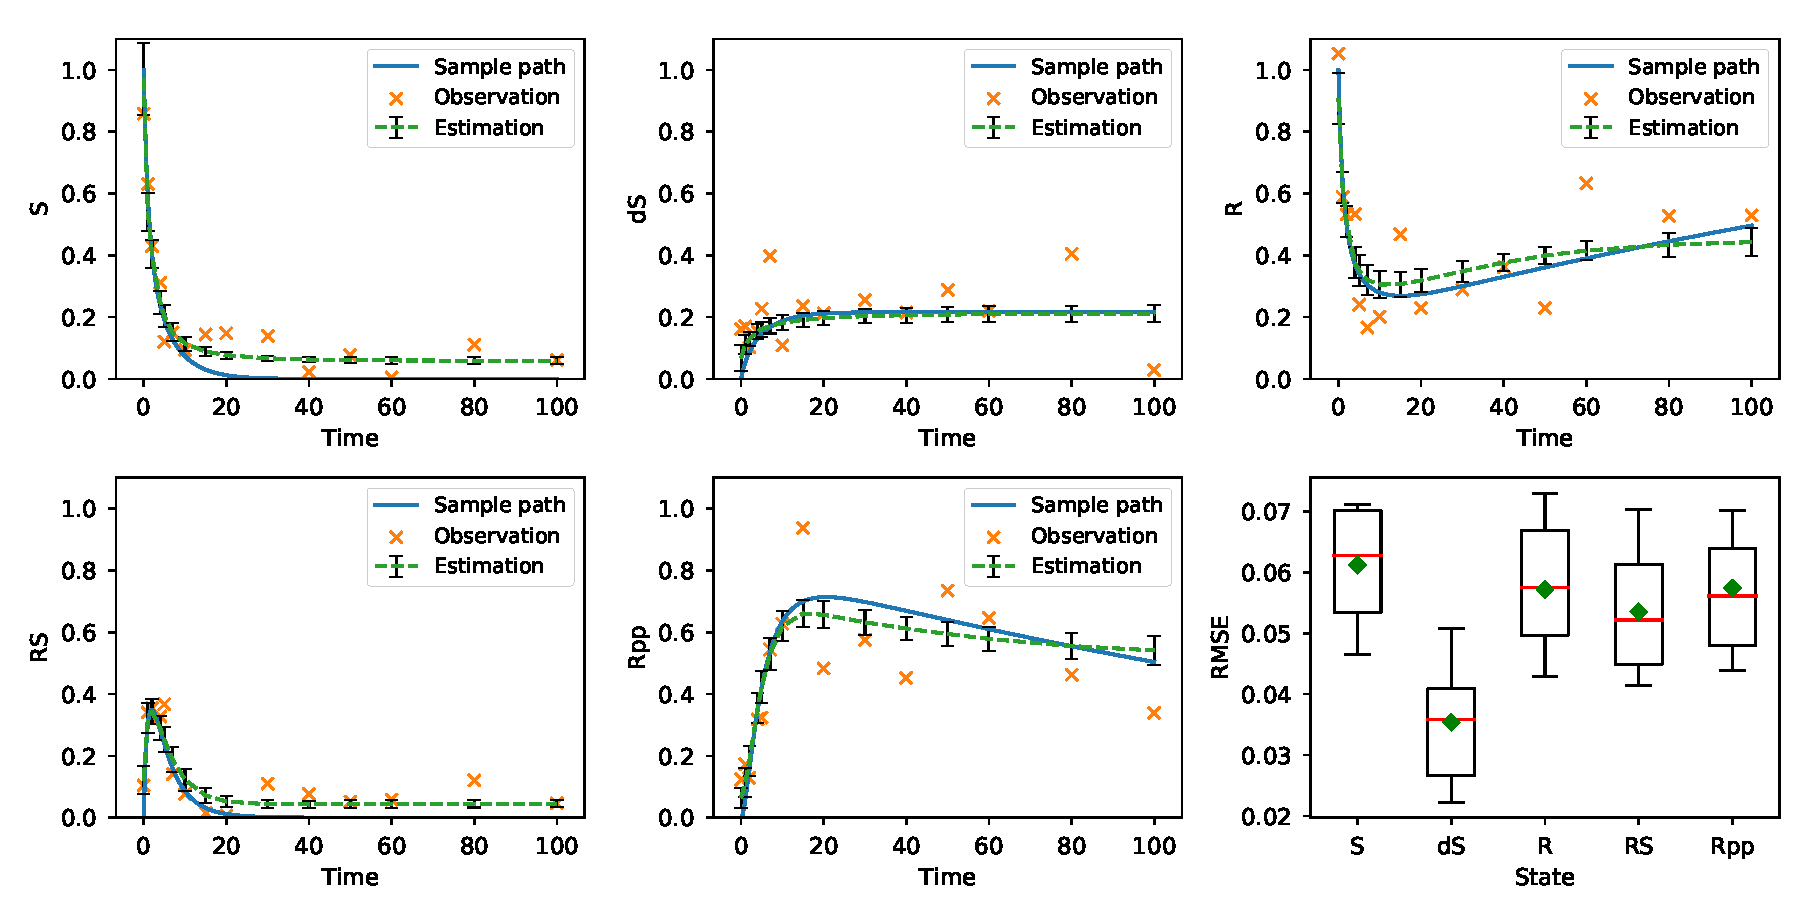
\includegraphics[width=\textwidth]{graphics/protein-states-without-km}
    \caption{State estimation results for the protein signaling transduction pathway model with the parameter $K_m$ set to constant. The ground truth is shown as the blue line. The observations, when available, are shown as the orange crosses. The estimation is shown as the dotted green line. The error bars in the first five plots indicate one standard deviation. For the box plot, the median is indicated by the red line, while the mean is shown as the green diamond. The box shows the lower and upper quartiles, while the whiskers are the 5th and 95th percentiles.}
    \label{fig-protein-states-without-km}
\end{figure}

\begin{figure}
    \centering
    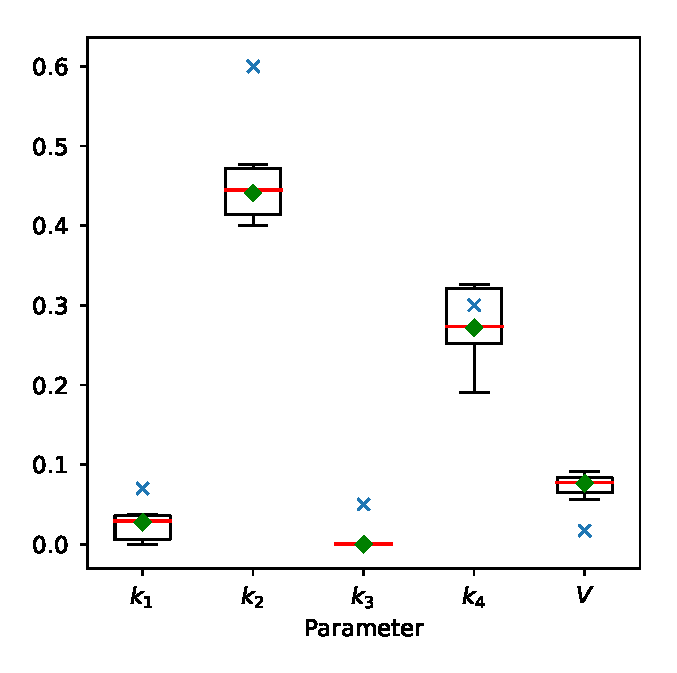
\includegraphics[width=0.48\textwidth]{graphics/protein-parameters-without-km}
    \caption{Parameter estimation results for the protein signaling transduction pathway model with the parameter $K_m$ set to constant. In the box plot, the median is indicated by the red line, while the mean is shown as the green diamond. The box shows the lower and upper quartiles, while the whiskers are the 5th and 95th percentiles. The true parameter values are indicated by the blue crosses.}
    \label{fig-protein-parameters-without-km}
\end{figure}

In this experiment, the parameter $K_m$ is not inferred but all the states are directly inferred.
This setup includes the $Rpp$ state that violates the structural assumption, which is not possible using the \algovgmgp\ method.
The results after 10 independent repetitions are shown in \reffigure{\ref{fig-protein-states-without-km}} and \reffigure{\ref{fig-protein-parameters-without-km}}.
For state estimation, the overall trend of the states is captured by the learning algorithm.
Since there are much fewer observations toward the end of the time point, the prediction becomes worse.
The parameter estimation result is not ideal in comparison to the states.

\subsubsection*{Partial observation}

\begin{figure}
    \centering
    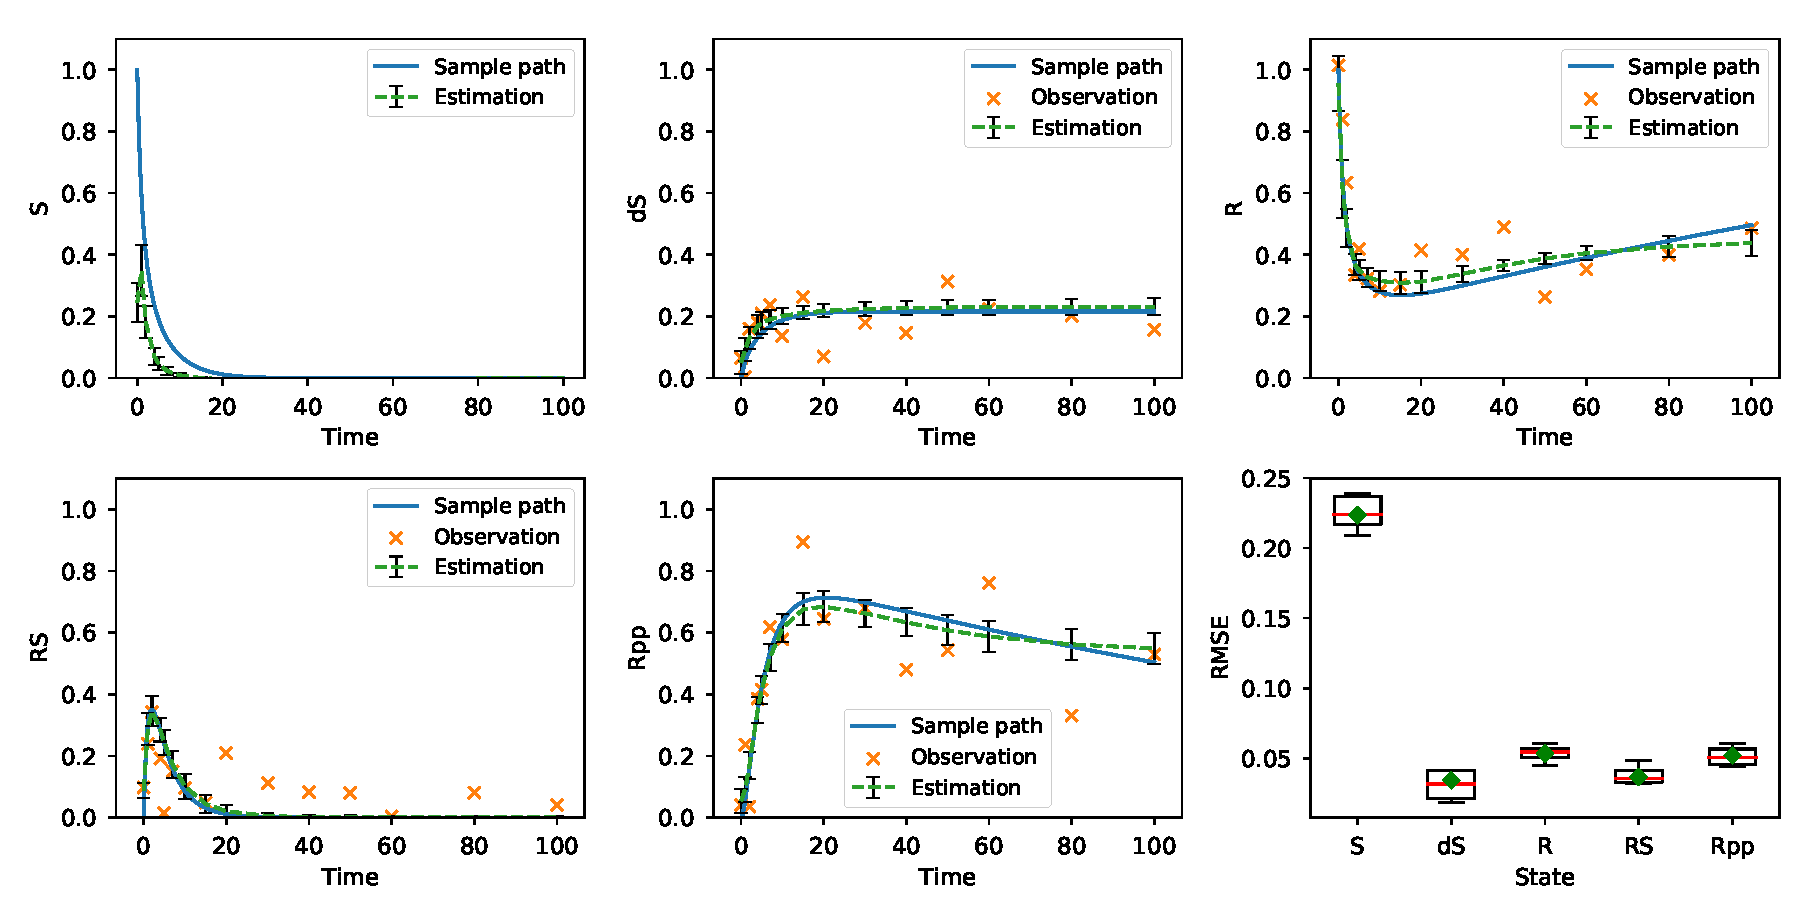
\includegraphics[width=\textwidth]{graphics/protein-states-partial-without-km}
    \caption{State estimation results for the protein signaling transduction pathway model with the parameter $K_m$ set to constant and the state $S$ unobservable. The ground true is shown as the blue line. The observations, when available, are shown as the orange crosses. The estimation is shown as the dotted green line. The error bars in the first five plots indicate one standard deviation. For the box plot, the median is indicated by the red line, while the mean is shown as the green diamond. The box shows the lower and upper quartiles, while the whiskers are the 5th and 95th percentiles.}
    \label{fig-protein-states-partial-without-km}
\end{figure}

\begin{figure}
    \centering
    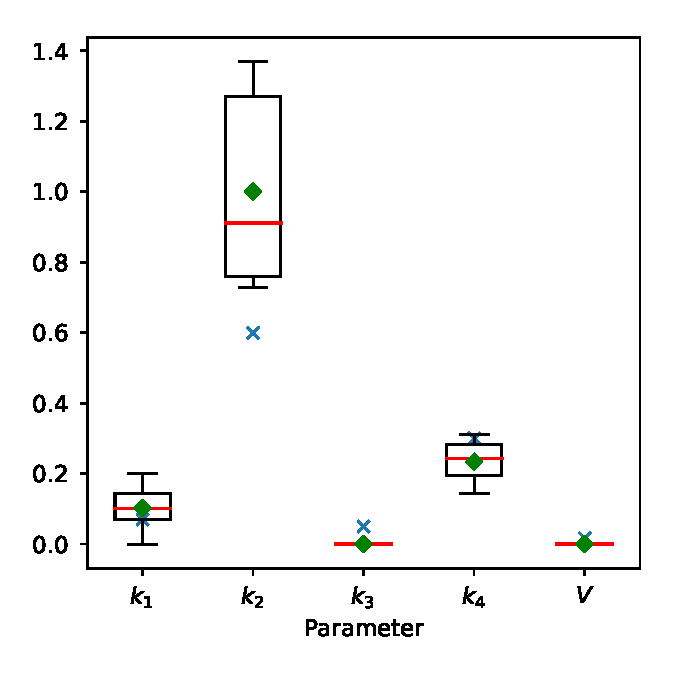
\includegraphics[width=0.48\textwidth]{graphics/protein-parameters-partial-without-km}
    \caption{Parameter estimation results for the protein signaling transduction pathway model with the parameter $K_m$ set to constant and the state $S$ unobservable. In the box plot, the median is indicated by the red line, while the mean is shown as the green diamond. The box shows the lower and upper quartiles, while the whiskers are the 5th and 95th percentiles. The true parameter values are indicated by the blue crosses.}
    \label{fig-protein-parameters-partial-without-km}
\end{figure}

To increase the difficult of the problem, the observations on the state $S$ is masked out.
The results after 10 independent repetitions is shown in \reffigure{\ref{fig-protein-states-partial-without-km}} and \reffigure{\ref{fig-protein-parameters-partial-without-km}}.
Given even less observations, the accuracy of both state and parameter estimation become worse.
From \reffigure{\ref{fig-protein-states-partial-without-km}} it can be seen that gradient model indeed does provide some guidance on the estimation of the state $S$.

\section{Lorenz 96 model}
\label{sec-lorenz-96}

As a minimalistic weather forecast model, the \emph{Lorenz 96} model \citep{lorenz1996predictability} is another widely used benchmark system due to its chaotic behavior under certain configurations and its flexibility to scale to large numbers of states.
A $K$-dimensional deterministic Lorenz 96 dynamical system is defined for $k = \mrange{1}{K}$, state-wise as follows:
\begin{align}
    \dymdxktn{k}{}
     & = (\dymxktn{k+1}{} - \dymxktn{k-2}{})\dymxktn{k-1}{} - \dymxktn{k}{} + F
    \label{eq-lorenz-96-drift}
\end{align}
where $\dymxktn{-1}{} = \dymxktn{K-1}{}$, $\dymxktn{0}{} = \dymxktn{K}{}$, $\dymxktn{K+1}{}=\dymxktn{1}{}$, and $F \in \R$ is the parameter controlling the behavior of the system.
When $F < 0.895$, the states decay into a steady value equal to $F$; when $F$ is between 0.895 and 4.0, the states are periodic; when $F \geqslant 4.0$, the system exhibits chaotic behavior \citep{vrettas2015variational}.
An example of the trajectories of a 10-dimensional deterministic Lorenz 96 model is shown in \reffigure{\ref{fig-lorenz-96-trajectories}}.

\begin{figure}
    \centering
    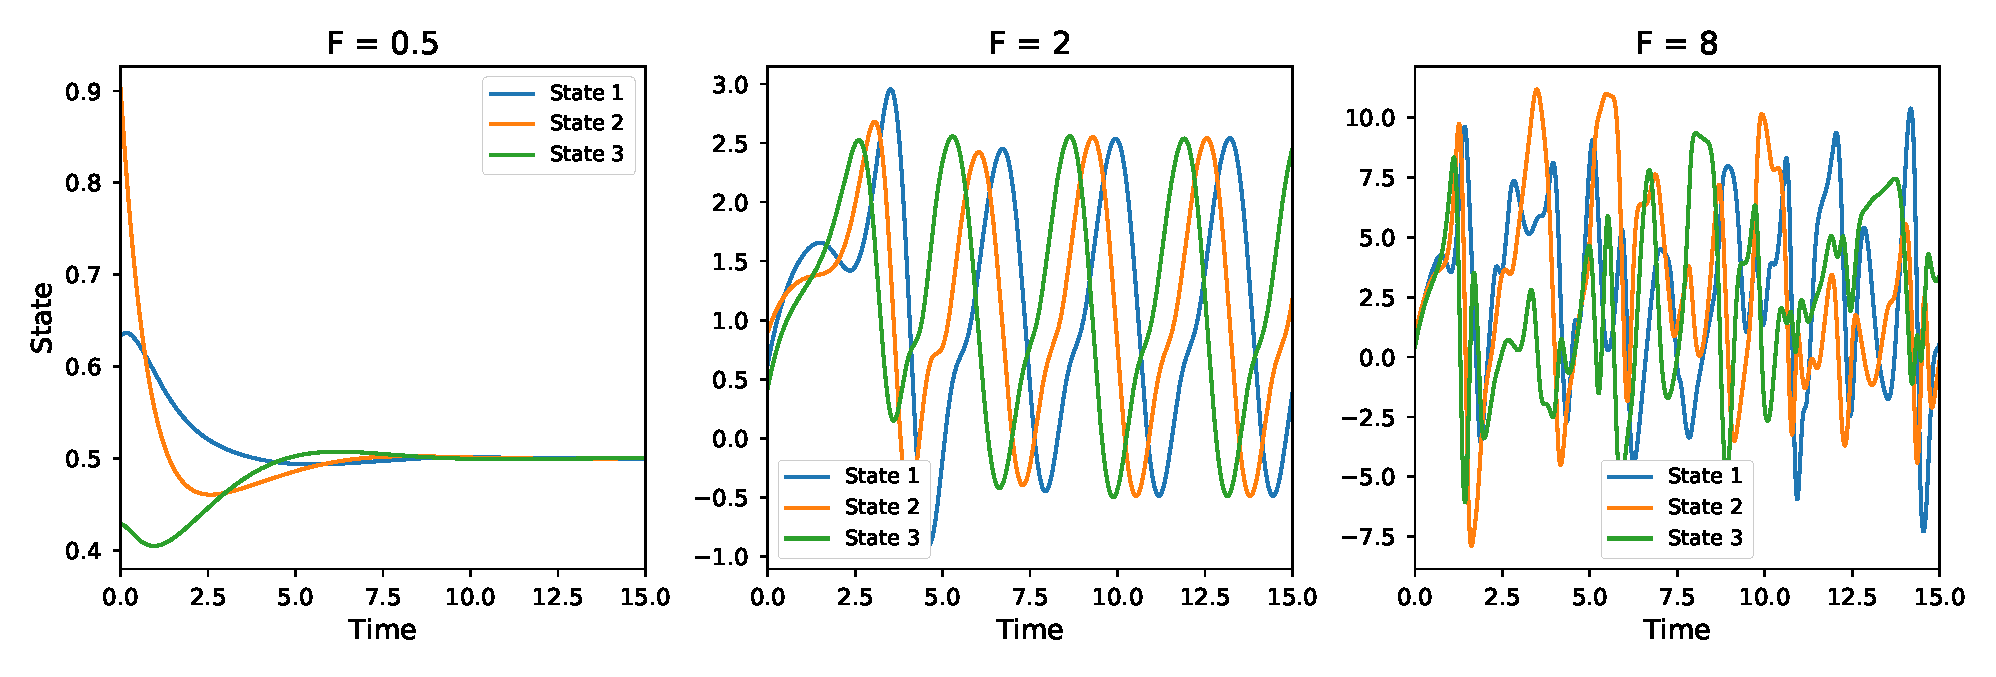
\includegraphics[width=\textwidth]{graphics/lorenz-96-trajectories}
    \caption{Trajectories of the 1st, 2nd and 3rd dimensions of a 10-dimensional deterministic Lorenz 96 model with different parameter values. The numerical integration is carried out from time 0 to 15 with a step size of 0.01.}
    \label{fig-lorenz-96-trajectories}
\end{figure}

The experiments in this section are mainly concerned about the stochastic Lorenz 96 model, which can be obtained by simply including a noise process as described in \refsection{\ref{sec-sdes}}.
Experiments about its deterministic counterpart can be found in \cite{gorbach2017scalable}.
In the following, we compare the results from the \algolpmfsde\ and the \algovgpamf\ methods.

\subsubsection*{Experimental setup}

Following \cite{vrettas2015variational}, \reftable{\ref{table-lorenz-96-setup}} shows the experimental setup to generate sample paths and to collect observations.
The sample paths are generated by the \algovgpamf\ MATLAB code, which uses the first order Euler-Maruyama scheme.
To avoid exploiting the special structure of the drift function \refequationp{\ref{eq-lorenz-96-drift}}, the observed states are selected randomly.
After observations are collected, the data files are converted into the format compatible with the \algolpmfsde\ source code.

\begin{table}
\centering
\caption{Experimental setup to generate sample paths and to collect observations for the stochastic Lorenz 96 model. The system dimension is denoted by $K$ and the number of observable dimensions is $K_{obs}$. Based on the drift parameter $F$ and the diffusion noise, the sample paths are generated from time $t_0$ to $t_T$ with a step size of $\delta t$. The observation noise variance $\dymsigmak{k}^2$ and the diffusion noise variance $\sderhoq{k}^2$ are assumed to be the identical for each state. For each time unit, $freq_{obs}$ denotes the number observations to be collected, which are equally distributed over the time line.}
\label{table-lorenz-96-setup}
\begin{tabular}{|c|c|c|c|c|c|c|c|c|}
\hline
$K$ & $K_{obs}$ & $t_0$ & $t_T$ & $\delta t$ & $F$ & $\dymsigmak{k}^2$  & $\sderhoq{k}^2$ & $freq_{obs}$ \\ \hline
500 & 325 (65\%) & 0 & 4 & 0.01 & 8 & 1 & 4 & 8 \\ \hline
\end{tabular}
\end{table}

Note that the system dimension is scaled down from 1000 to 500 due to time constraints.
Accordingly, the number of observed states is scaled down proportionally.
Nevertheless, it is still very interesting to quantify the scalability of the \algolpmfsde\ solution, which will be examined in detail in a separate experiment later.

For each SDE sample path, the \algolpmfsde\ method averages individual inference results from 100 independently generated RODE sample paths to obtain an ensemble solution.
The RODE sample paths are estimated in parallel on the ETH Euler cluster\footnote{\url{https://scicomp.ethz.ch/wiki/Euler}}.
Only 1 CPU core and 2 GB of memory are allocated to each inference.
For this experiment, the RODE states are estimated using the gradient-based method while the parameters are calculated in closed-form.

On the other hand, the \algovgpamf\ code is deployed on a desktop with an Intel i5 quad-core CPU and 16 GB of memory.
We also note that thread pooling is used to utilize all the CPU resources for the \algovgpamf\ implementation, which is not the case for \algolpmfsde.

\subsubsection*{State estimation}

\begin{figure}
    \centering
    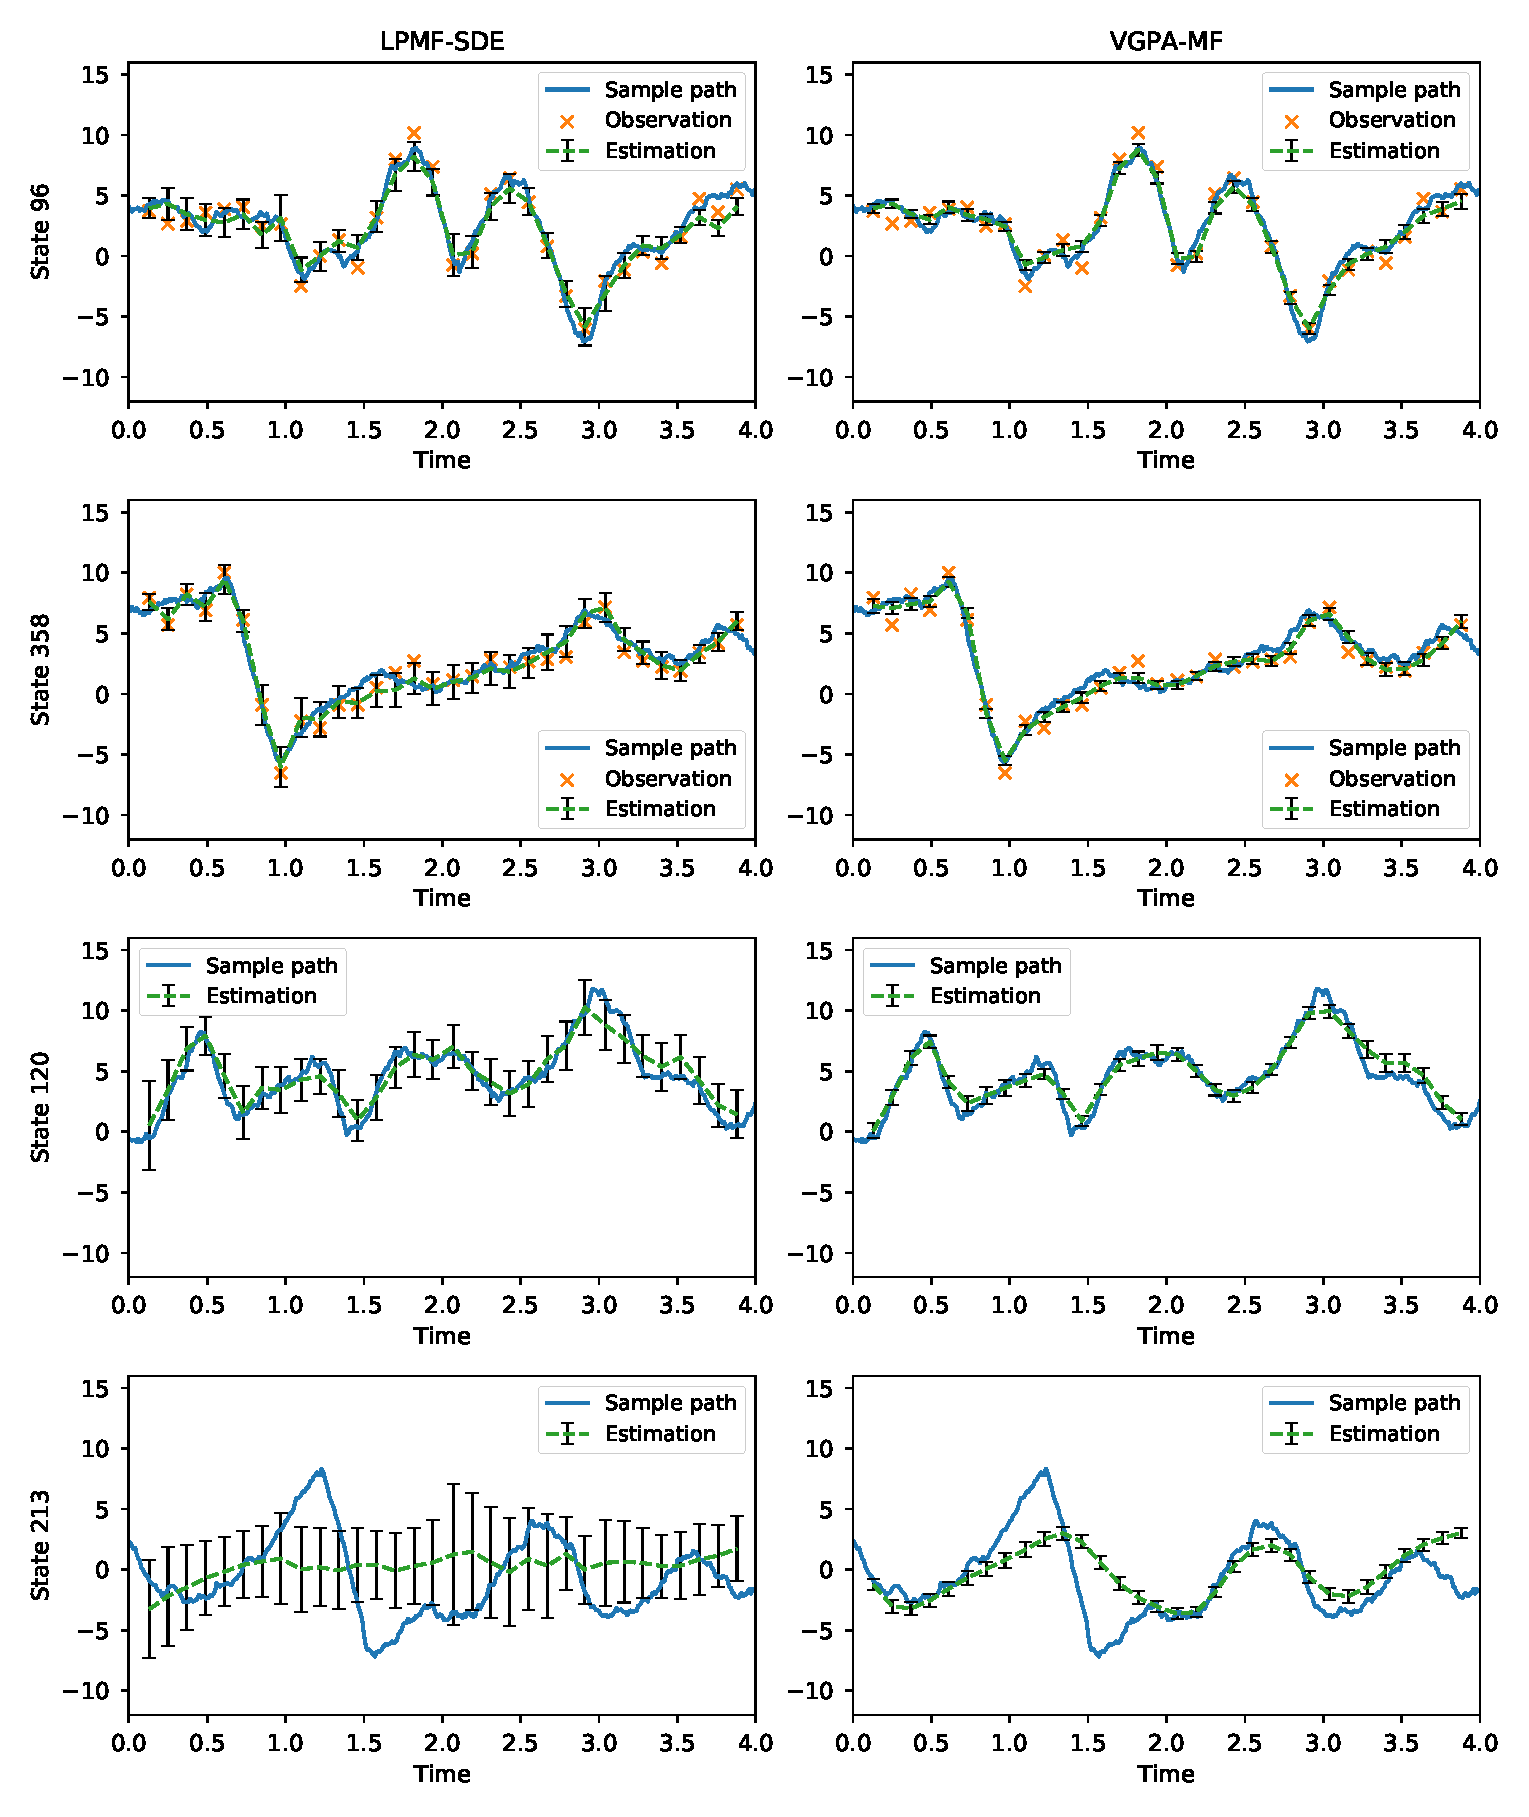
\includegraphics[width=\textwidth]{graphics/lorenz-96-states}
    \caption{State estimation results for 4 selected states from the 500-dimensional stochastic Lorenz 96 model. Among the 500 states, 325 are observed. The left column shows the result using the \algolpmfsde\ method, while the right column contains the result based on the \algovgpamf\ algorithm. In the four rows, state 96 and its neighboring states are directly observed; state 358 and only one side of its neighbors are directly observed; state 120 is not observed but its neighbors are;  state 213 and its neighbors are all unobserved. The ground truth is shown as a solid blue line. The mean of estimation is drawn as a dotted green line together with the error bars indicating one standard deviation. Observations, when available, are indicated by the orange crosses.}
    \label{fig-lorenz-96-states}
\end{figure}

\reffigure{\ref{fig-lorenz-96-states}} shows an example of the state inference result for the stochastic Lorenz 96 model using both methods.
For observed states, the mean values of the predictions from both methods are very close to the ground truth, while the \algovgpamf\ method tends to have lower variance.
For unobserved states, the accuracy of both methods depends on the amount of available information that is directly related to them.
As indicated by the drift function \refequationp{\ref{eq-lorenz-96-drift}}, the states are only coupled with their  neighbors for the Lorenz 96 model.
Therefore, estimation on an unobserved state can be reasonably good when its neighbors are observed, e.g.\ state 120 has observed neighbors 121, 122, 123, etc.
Estimation can fail when the neighbors of that state are also unobserved so that they are unable to provide sufficient information to the algorithm, e.g.\ the true trajectory of state 213 cannot be recovered since states 211 to 215 are all unobserved.
As expected, the uncertainty about the estimation for unobserved states is higher than that for the observed states, which is indicated by the wider error bars.

In order to better quantify the difference between both methods, 10 independent Lorenz 96 SDE sample paths are generated. 
For each SDE sample path, a set of observations is collected, and then the above experiment is repeated.
The root mean square error (RMSE) is used as the accuracy measure, and the RMSEs for observed and unobserved states are considered separately.
The formulas for the RMSEs are
\begin{align}
    RMSE_{obs} 
    & = \frac{1}{K_{obs}}\sum_{k\in \mathcal{S}_{obs}}{\sqrt{
        \frac{1}{N}\sum_{n=1}^N{
            (\dymxhatktn{k}{n} - \dymxktn{k}{n})^2
        }
    }}
    \\
    RMSE_{unobs} 
    & = \frac{1}{K_{unobs}}\sum_{k\in \mathcal{S}_{unobs}}{\sqrt{
        \frac{1}{N}\sum_{n=1}^N{
            (\dymxhatktn{k}{n}-\dymxktn{k}{n})^2
        }
    }}    
\end{align}
where $K_{obs}$ and $K_{unobs}$ indicate the number of observed and unobserved states respectively with $\mathcal{S}_{obs}$ and $\mathcal{S}_{obs}$ as the corresponding sets containing the state indices, $N$ is the total number of observations for each dimension, and $\dymxhatktn{k}{n}$ and $\dymxktn{k}{n}$ are the predicted and true values for the $k$-th state at time point $t$ respectively.

\begin{figure}
    \centering
    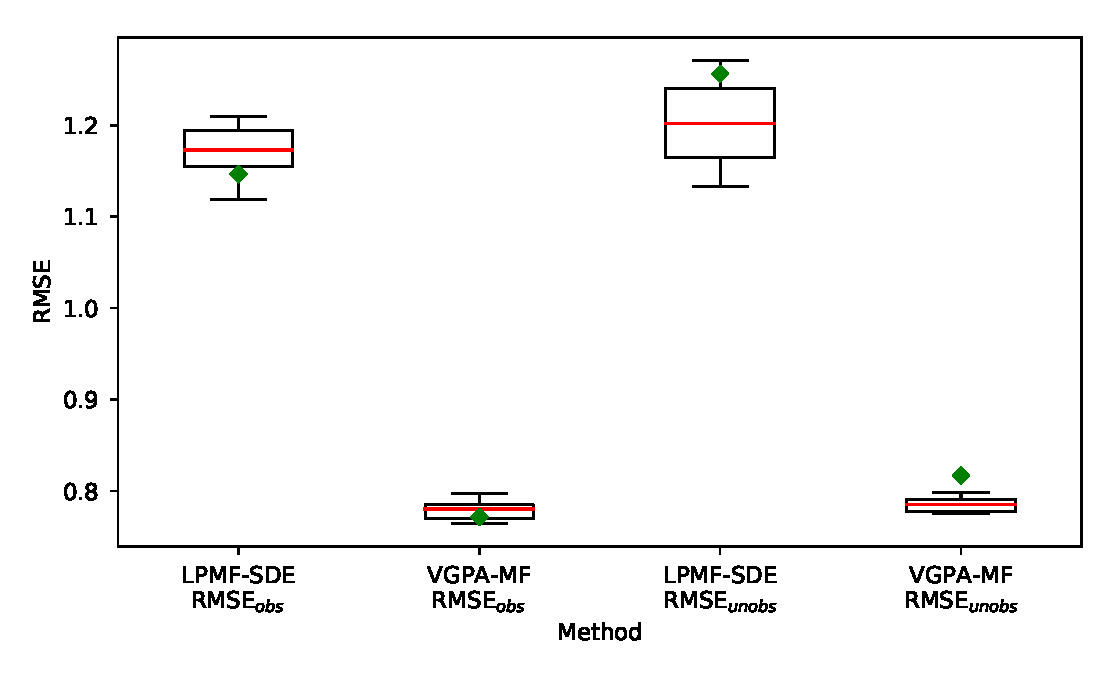
\includegraphics[width=0.8\textwidth]{graphics/lorenz-96-states-boxplot}    
    \caption{Box plot for the RMSEs of state estimation over 10 independent repetitions using sample paths from the 500-dimensional stochastic Lorenz 96 model with 325 observable states. The RMSEs of observed and unobserved states are calculated separately. In the box plot, the median is indicated by the red line, while the mean is shown as the green diamond. The box shows the lower and upper quartiles, while the whiskers are the 5th and 95th percentiles.}
    \label{fig-lorenz-96-state-boxplot}
\end{figure}

The results of the 10 independent repetitions are summarized in \reffigure{\ref{fig-lorenz-96-state-boxplot}}.
At first glance, it is surprising that the \algovgpamf\ method has such low RMSE values.
This is partially because in the MATLAB code we have obtained, only state inference is carried out and the true drift parameter $F$ is given to the inference procedure.
However, the \algolpmfsde\ method is estimating both the states and parameters simultaneously.
Note that the \algovgpamf\ solution is fully capable of jointly estimating the states and parameters.
But as at the time of this writing, we have not obtained the code that computes the gradient of their variational free energy function w.r.t.\ the parameters in order to complete the required experiments.
Moreover, as claimed by \cite{vrettas2015variational}, their  solution can also estimate the diffusion noise, which is an advantage over the \algolpmfsde\ method and can be considered as a possible future extension to this work.
Considering the sparsity of the observations and that the observation noise variances are set to 1, we see some potential for the \algolpmfsde\ solution.

One shortcoming of the \algolpmfsde\ method in this experiment is that it only considers a single optimal value of the cost function found using gradient-based method when making predictions.
Depending on the initialization conditions and the complexity of the cost function, which is subject to the complexity of drift function, sometimes the optimization procedure be trapped in a local optimum.
As a consequence, even though the mean can be recovered reasonably well, the variance of the prediction is less under control.
Since currently only out-of-package second-order optimization techniques such as the \emph{truncated Newton method}, the \emph{dog-leg trust-region algorithm}, etc. \citep{nocedal2006numerical}, are used, further improvement on the optimization strategy can also be considered as an extension to the current work.

\subsubsection*{Parameter estimation}

This section only discusses parameter inference results using the \algolpmfsde\ method due to the lack of relevant files from the \algovgpamf\ MATLAB code as mentioned previously.
The result for a single SDE sample path is illustrated in \reffigure{\ref{fig-lorenz-96-parameters}}, while the result from the 10 dependent repetitions is summarized in \reffigure{\ref{fig-lorenz-96-parameters-boxplot}}.

\begin{figure}
    \centering
    \begin{subfigure}[b]{0.48\textwidth}
        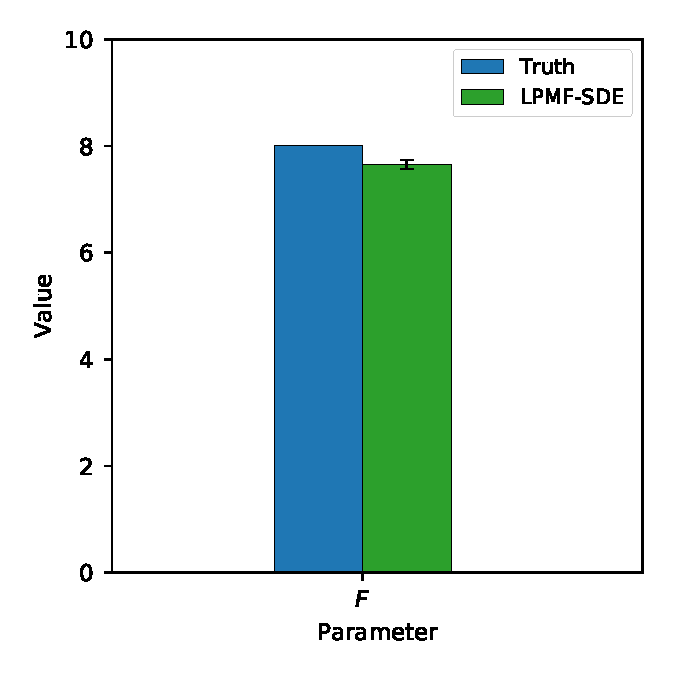
\includegraphics[width=\linewidth]{graphics/lorenz-96-parameters}
        \caption{\ }
        \label{fig-lorenz-96-parameters}
    \end{subfigure}
    \begin{subfigure}[b]{0.48\textwidth}
        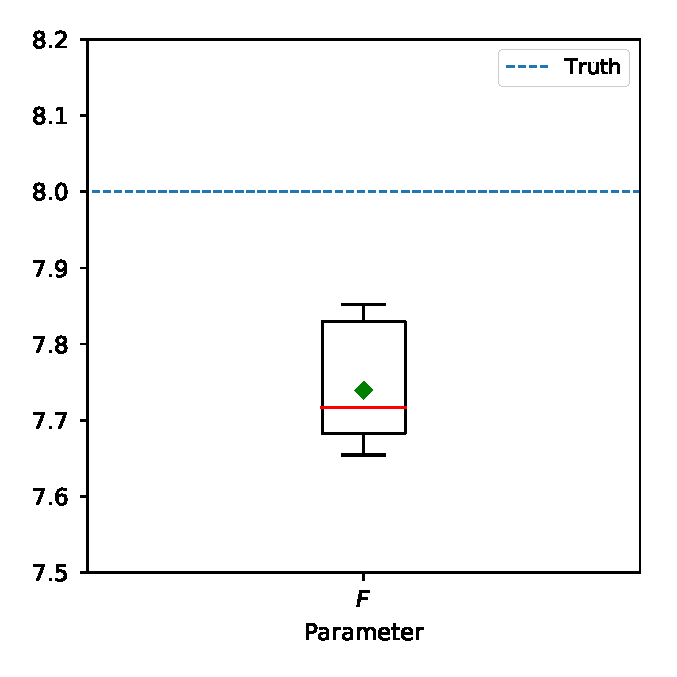
\includegraphics[width=\linewidth]{graphics/lorenz-96-parameters-boxplot}
        \caption{\ }
        \label{fig-lorenz-96-parameters-boxplot}
    \end{subfigure}
    \caption{Parameter estimation result using the \algolpmfsde\ algorithm for the 500-dimensional stochastic Lorenz 96 model with 325 observable states. (a) Estimation result for the SDE sample path shown in \reffigure{\ref{fig-lorenz-96-states}}. The blue bar indicates the true parameter value. The green bar shows the mean of estimation by averaging individual results from 100 RODE sample paths. The error bar indicates one standard deviation. (b) Box plots for parameter estimation over 10 independent repetitions. In the box plot, the median is indicated by the red line, while the mean is shown as the green diamond. The box shows the lower and upper quartiles, while the whiskers are the 5th and 95th percentiles. The dotted blue line indicates the true parameter value.}
    \label{fig-lorenz-96-parameters-group}    
\end{figure}

\reffigure{\ref{fig-lorenz-96-parameters}} shows that the estimation of the drift parameter $F$ is very close to the true value 8, and the variance is much lower in comparison to state estimation.
This is due to the fact that the Lorenz 96 model has only one drift parameter, which appears inside the drift function for each state.
Hence, the gradient matching model is able to obtain much more information about the drift parameter, despite the existence of unobserved states.
\reffigure{\ref{fig-lorenz-96-parameters-boxplot}} further shows that the mean values of parameter estimation over the 10 independent repetitions are narrowly distributed.
But in general, the \algolpmfsde\ method tends to underestimate the parameter value.

\subsubsection*{Runtime performance}

\begin{figure}
    \centering
    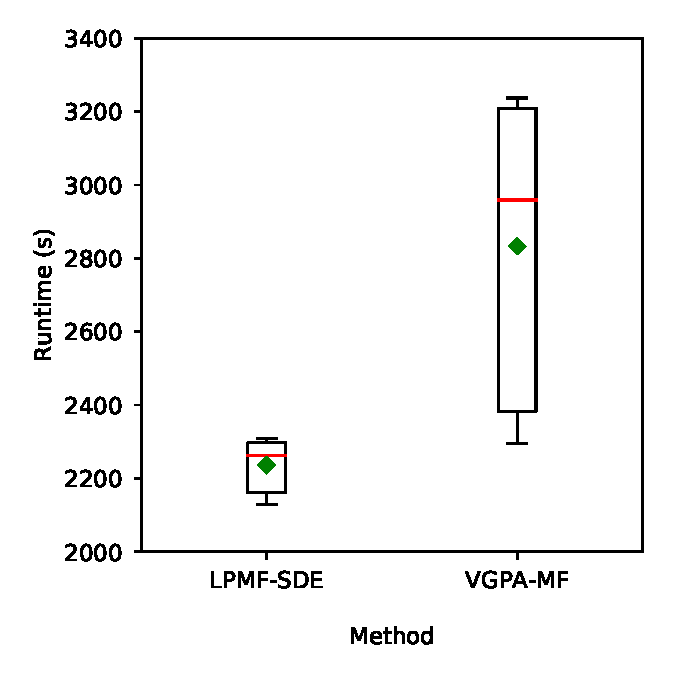
\includegraphics[width=0.48\textwidth]{graphics/lorenz-96-runtime-boxplot}
    \caption{Box plot for the runtimes over 10 repetitions using independent sample paths from the stochastic Lorenz 96 model. The median is indicated by the red line, while the mean is shown as the green diamond. The box shows the lower and upper quartiles, while the whiskers are the 5th and 95th percentiles.}        
    \label{fig-lorenz-96-runtime-boxplot}
\end{figure}

For the SDE sample path shown in \reffigure{\ref{fig-lorenz-96-states}}, the average runtime for the \algolpmfsde\ algorithm to solve one RODE sample path is 2309 seconds with a standard deviation of around 128 seconds, while the runtime for the \algovgpamf\ method takes 3232 seconds.
As the current \algovgpamf\ MATLAB code only runs the state smoothing algorithm, it is expected to be much more computationally intensive when parameter estimation is carried out simultaneously, since the forward-backward loop has to be entered many times until convergence.

\reffigure{\ref{fig-lorenz-96-runtime-boxplot}} summarizes the average runtimes for \algolpmf\ to solve one RODE sample path and the runtimes for \algovgpamf\ to complete one iteration of state smoothing over the 10 independent repetitions.
It shows that the \algolpmfsde\ solution performs consistently faster and more stably than its counterpart, as indicated by lower median runtime value and the narrower distribution.

To conclude, the \algolpmfsde\ algorithm requires much less resources and also runs faster for inference on one RODE sample path.
However, the ensemble nature of the \algolpmfsde\ strategy relies on averaging results from a large number RODE estimations, which could increase the computational requirements significantly.
Nevertheless, given the availability of computer farms and the ease of setting up distributed inference pipeline nowadays, the parallelism requirement for the \algolpmfsde\ solution can be easily satisfied. 


\subsubsection*{Scalability}

\begin{figure}
    \centering
    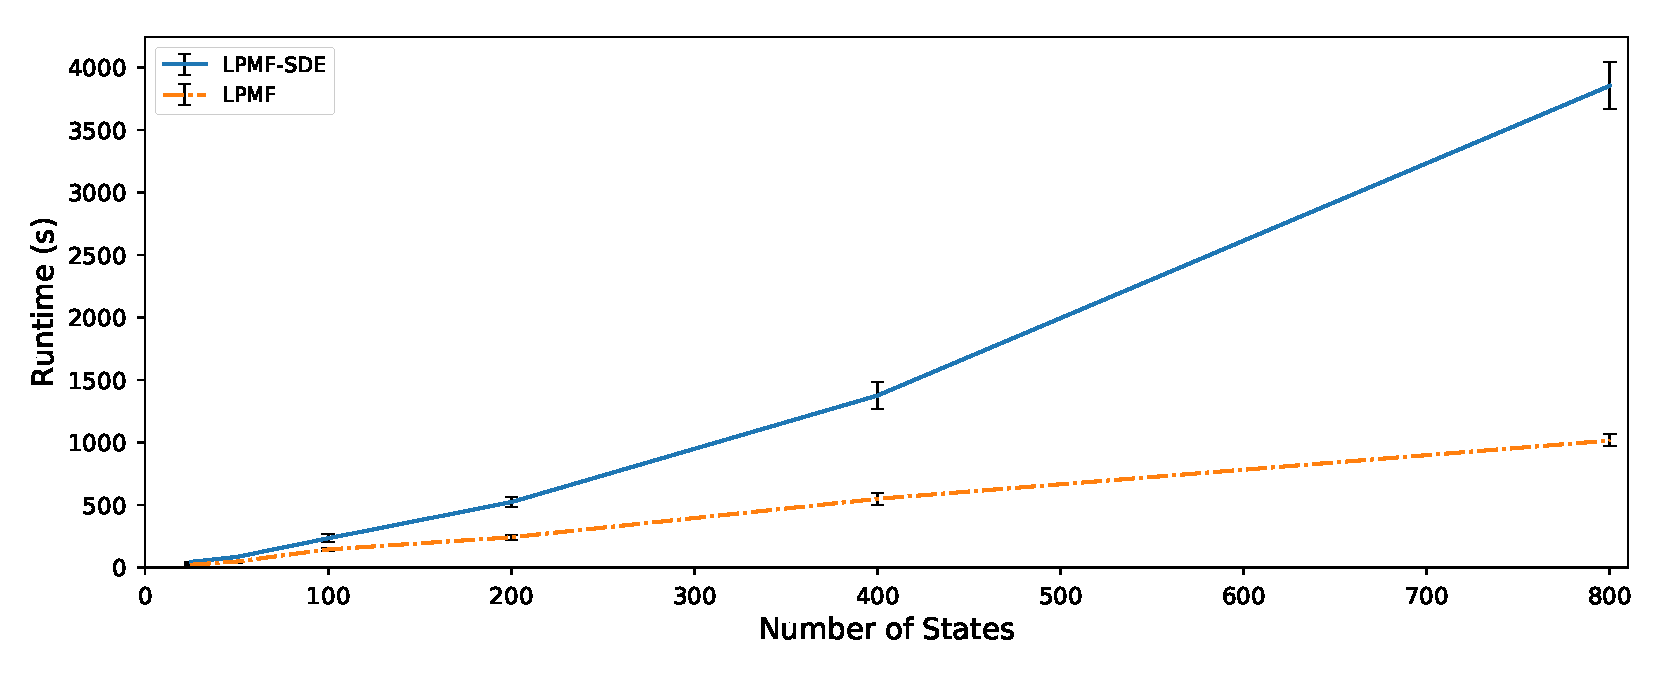
\includegraphics[width=\textwidth]{graphics/lorenz-96-scalability}
    \caption{Scalability of the \algolpmfsde\ algorithm versus its deterministic counterpart, i.e.\ \algolpmf, as the dimensionality of the system increases. For the \algolpmfsde\ method, the blue line indicates the average interpolated runtime to inference one RODE sample path over 10 independent RODE sample paths by connecting the measurements at 25, 50, 100, 200, 400 and 800. For the \algolpmf\ method, the orange line is obtained by connecting the averages of 10 independent runs on the same ODE trajectory with different observations at the same measurement points. The error bars in both setups indicate one standard deviation.}
    \label{fig-lorenz-96-scalability}
\end{figure}

As mentioned by \cite{gorbach2017scalable}, inference on the deterministic Lorenz 96 model with 1000 states using their \algovgmgp\ solution completes within 400 seconds on average.
However, the \algolpmfsde\ method, which extends their methodology, takes on average more than 2200 seconds for one RODE sample path with only 500 states, as shown in \reffigure{\ref{fig-lorenz-96-runtime-boxplot}}.
It is therefore interesting to re-examine the scalability of the \algolpmfsde\ solution.

First, we noticed during implementation that the performance of the \algolpmf\ method for ODEs is comparable to the \algovgmgp\ method.
The major difference between \algolpmfsde\ and \algolpmf\ is the introduction of a stochastic Ornstein-Uhlenbeck process into the vector field of the ODEs.
To reveal the influence of the stochastic process on the inference procedure, the following experiment compares side-by-side the performance of the \algolpmfsde\ method running on the stochastic Lorenz 96 model with the performance of the \algolpmf\ method running on its deterministic counterpart as the number of states increases.

Specifically, measurements are taken with a system dimensionality of 25, 50, 100, 200, 400, and 800 with the number of observed states kept at 65 percent of the total number of states.
Using the same setup in \reftable{\ref{table-lorenz-96-setup}}, except that the diffusion noise is not used for the Lorenz 96 ODEs, the \algolpmfsde\ algorithm is tested with 10 independent RODE sample paths while the \algolpmf\ method is tested with 10 independent observation sets from the same ODE trajectory for each system dimensionality.
The experiments are all conducted on the Euler cluster with the same hardware configuration.

As can be seen from \reffigure{\ref{fig-lorenz-96-scalability}}, benefiting from the efficient implementation of the gradient and Hessian evaluation subroutines, the gradient-based \algolpmf\ method incurs only a slightly higher performance penalty than the closed-form solution from \algovgmgp.
Also, the runtime seems to increase linearly as the number of states increases.
On the other hand, the performance of the \algolpmfsde\ method degrades much faster than \algolpmf, and the gap between them become larger as the number of states increases.
The cause of this phenomenon requires further investigation but a plausible explanation is the complication of the optimization objective after the introduction of the stochastic process into the vector field.

\section{Lorenz 63 model}
\label{sec-lorenz-63}

The last dynamical system examined in this chapter is the stochastic version of the \emph{Lorenz 63} model \citep{lorenz1963deterministic}, which is a low dimensional mathematical model for thermal convection in the atmosphere.
The vector field of the deterministic Lorenz 63 is defined as follows:
\begin{align}
    \dymf
    & =
    \begin{bmatrix}
        \dot{x}(t)
        \\ 
        \dot{y}(t)
        \\
        \dot{z}(t)
    \end{bmatrix}
    =
    \begin{bmatrix}
        \sigma(y(t) - x(t))
        \\
        x(t)(\rho - z(t)) - y(t)
        \\
        x(t)y(t) - \beta z(t)
    \end{bmatrix}
    \label{eq-lorenz-63-odes}
\end{align}
where the state vector is given by $\dymx = [x(t), y(t), z(t)]^\top \in \R^3$, and $\dymtheta = [\sigma, \rho, \beta]^\top \in \R^3$ is the parameter vector controlling the system behavior.
Although consisting of only 3 states, this model is highly nonlinear and exhibits chaotic behavior under certain parameter configurations.

Correspondingly, the stochastic Lorenz 63 model with a state-specific, additive noise process is given by
\begin{align}
    \sdedx = \sdef \sdedt + \sdeSigma^\frac{1}{2}\sdedwt
\end{align}
where $\sdef$ is defined in \refequationp{\ref{eq-lorenz-63-odes}}, $\sdeSigma \in \R^{3 \times 3}$ is a diagonal matrix containing the diffusion noise variance, and $\sdewt$ is a 3-dimensional standard Wiener process.
Using the parameter set $[10, 28, \frac{8}{3}]^\top$, which is well-known for its resulting chaotic behavior, a sample path is shown in \reffigure{\ref{fig-lorenz-63-sample-path}}.

\begin{figure}
    \centering
    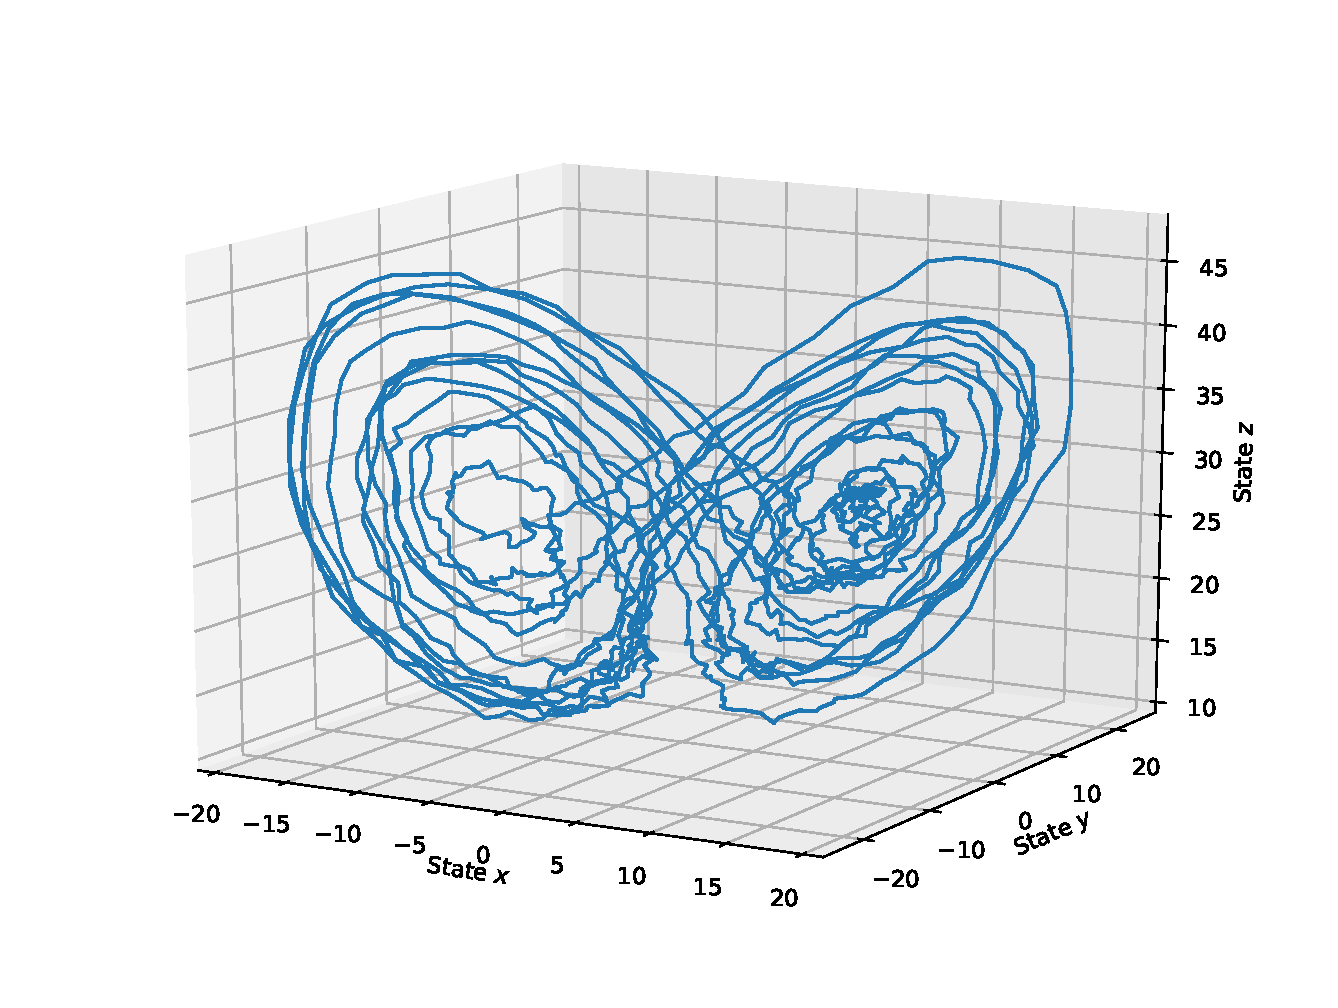
\includegraphics[width=0.8\textwidth]{graphics/lorenz-63-sample-path}
    \caption{Sample path for the stochastic Lorenz 63 model generated based on the parameter values $[\sigma, \rho, \beta]^\top = [10, 28, \frac{8}{3}]^\top$ and the diffusion noise variances $\sderhoq{1}^2 = \sderhoq{2}^2 = \sderhoq{3}^2 = 10$. The integration is performed from time 0 to 20 with a step size of 0.01.}
    \label{fig-lorenz-63-sample-path}
\end{figure}

\subsubsection*{Comparison algorithm}

In order to make comparison, a minimalistic MAP estimation of the drift parameters based on \cite[Table 3]{vrettas2011estimating} is self-implemented\footnote{\url{https://github.com/ruiixu23/VGPA}} by extending the Python source code\footnote{\url{https://github.com/vrettasm/VGPA}} for the \algovgpa\ algorithm.
In the following, the abbreviation \algovgpamap\ is used to refer to this extension.

The extension consists of an inner loop and an outer loop.
The inner loop enhances state estimation by running the \algovgpa\ smoothing algorithm to compute the optimal approximate state posterior, based on the current estimation of the parameters.
The outer loop then takes a gradient step to update the parameters.
This procedure is repeated until either the gradient over the parameters vanishes or the state estimation from the inner loop does not improve further significantly. 
Details of the algorithm can be found in \cite[Section 5.2]{vrettas2011estimating}.

Note that \cite{vrettas2011estimating} claim that the aforementioned algorithm can be similarly applied to the estimation of the diffusion noise covariance matrix $\sdeSigma$, which is not implemented here as the current \algolpmfsde\ method only supports inference on the drift parameters.
Also, the extension adopts a simple gradient update strategy with a fixed learning rate, which may lead to suboptimal result but can nonetheless be used as a baseline.

\subsubsection*{Experimental setup}

Adopting the experimental setup from \cite{vrettas2015variational}, the configuration used to generate sample paths and to collect observations is shown in \reftable{\ref{table-lorenz-63-setup}}.
Specifically, the sample paths are generated by the \algovgpa\ source code using the first order Euler-Maruyama method with a small step size to achieve higher accuracy.
After observations are collected, the data files are transformed into the format compatible with the \algolpmfsde\ method.

\begin{table}
\centering
\caption{Experimental setup to generate sample paths and to collect observations for the stochastic Lorenz 63 model. The system dimension is denoted by $K$ and the number of observable states is denoted by $K_{obs}$. Given the drift parameters $\sigma$, $\rho$, $\beta$ and the diffusion noise, the sample paths are generated from time $t_0$ to $t_T$ with a step size of $\delta t$. The variances of the observation noise $\dymsigmak{k}^2$ and the diffusion noise $\sderhoq{k}^2$ are assumed to be identical for each state. For each time unit, $freq_{obs}$ denotes the number of observations to be collected, which are equally distributed over the time line.}
\label{table-lorenz-63-setup}
\begin{tabular}{|c|c|c|c|c|c|c|c|c|}
\hline
$K$ & $K_{obs}$ & $t_0$ & $t_T$ & $\delta t$ & $\sigma, \rho, \beta$ & $\dymsigmak{k}^2$  & $\sderhoq{k}^2$ & $freq_{obs}$ \\ \hline
3 & 3 or 2 & 0 & 20 & 0.01 & $10, 28, \frac{8}{3}$ & 2 & 10 & 5 \\ \hline
\end{tabular}
\end{table}

In order to provide a fair comparison, both methods are deployed to the Euler cluster using the same hardware configuration described in \refsection{\ref{sec-lorenz-96}}.
For \algolpmfsde, 100 independent RODE sample paths are solved to obtain an ensemble result for one SDE sample path.
The states are optimized using a gradient-based method while the parameters are calculated analytically with mirroring of negative parameters\footnote{The mirroring of negative parameters is a heuristic solution. A better approach would be the enforcement of positivity constraint.}.
For \algovgpamap, the learning rate is fixed to 0.001, the maximum number of iterations is 250, and the stopping criteria are the decrease in the total variational free energy and the \emph{L2 norm} of the change to the drift parameters with a threshold of $10^{-6}$.
We noticed that all the experiments from \algovgpamap\  reached the maximum number of 250 iterations.
After manual examination, the result at the 80th iteration is used for the following comparisons.

It would be interesting to compare these two methods with one unobserved state.
Unfortunately, the smoothing result from the \algovgpa\ algorithm with unobserved state is not ideal from preliminary examination.
Therefore, a comparison with full state observability is provided.
But in order to demonstrate that the \algolpmfsde\ solution is capable of handling partial observations, an additional experiment is conducted by masking out the observations for state $y$.
To distinguish the two scenarios, we use \algolpmfsdef\ and  \algolpmfsdep\ to refer to the fully and partially observable cases respectively.

\subsubsection*{State estimation}

\begin{figure}
    \centering
    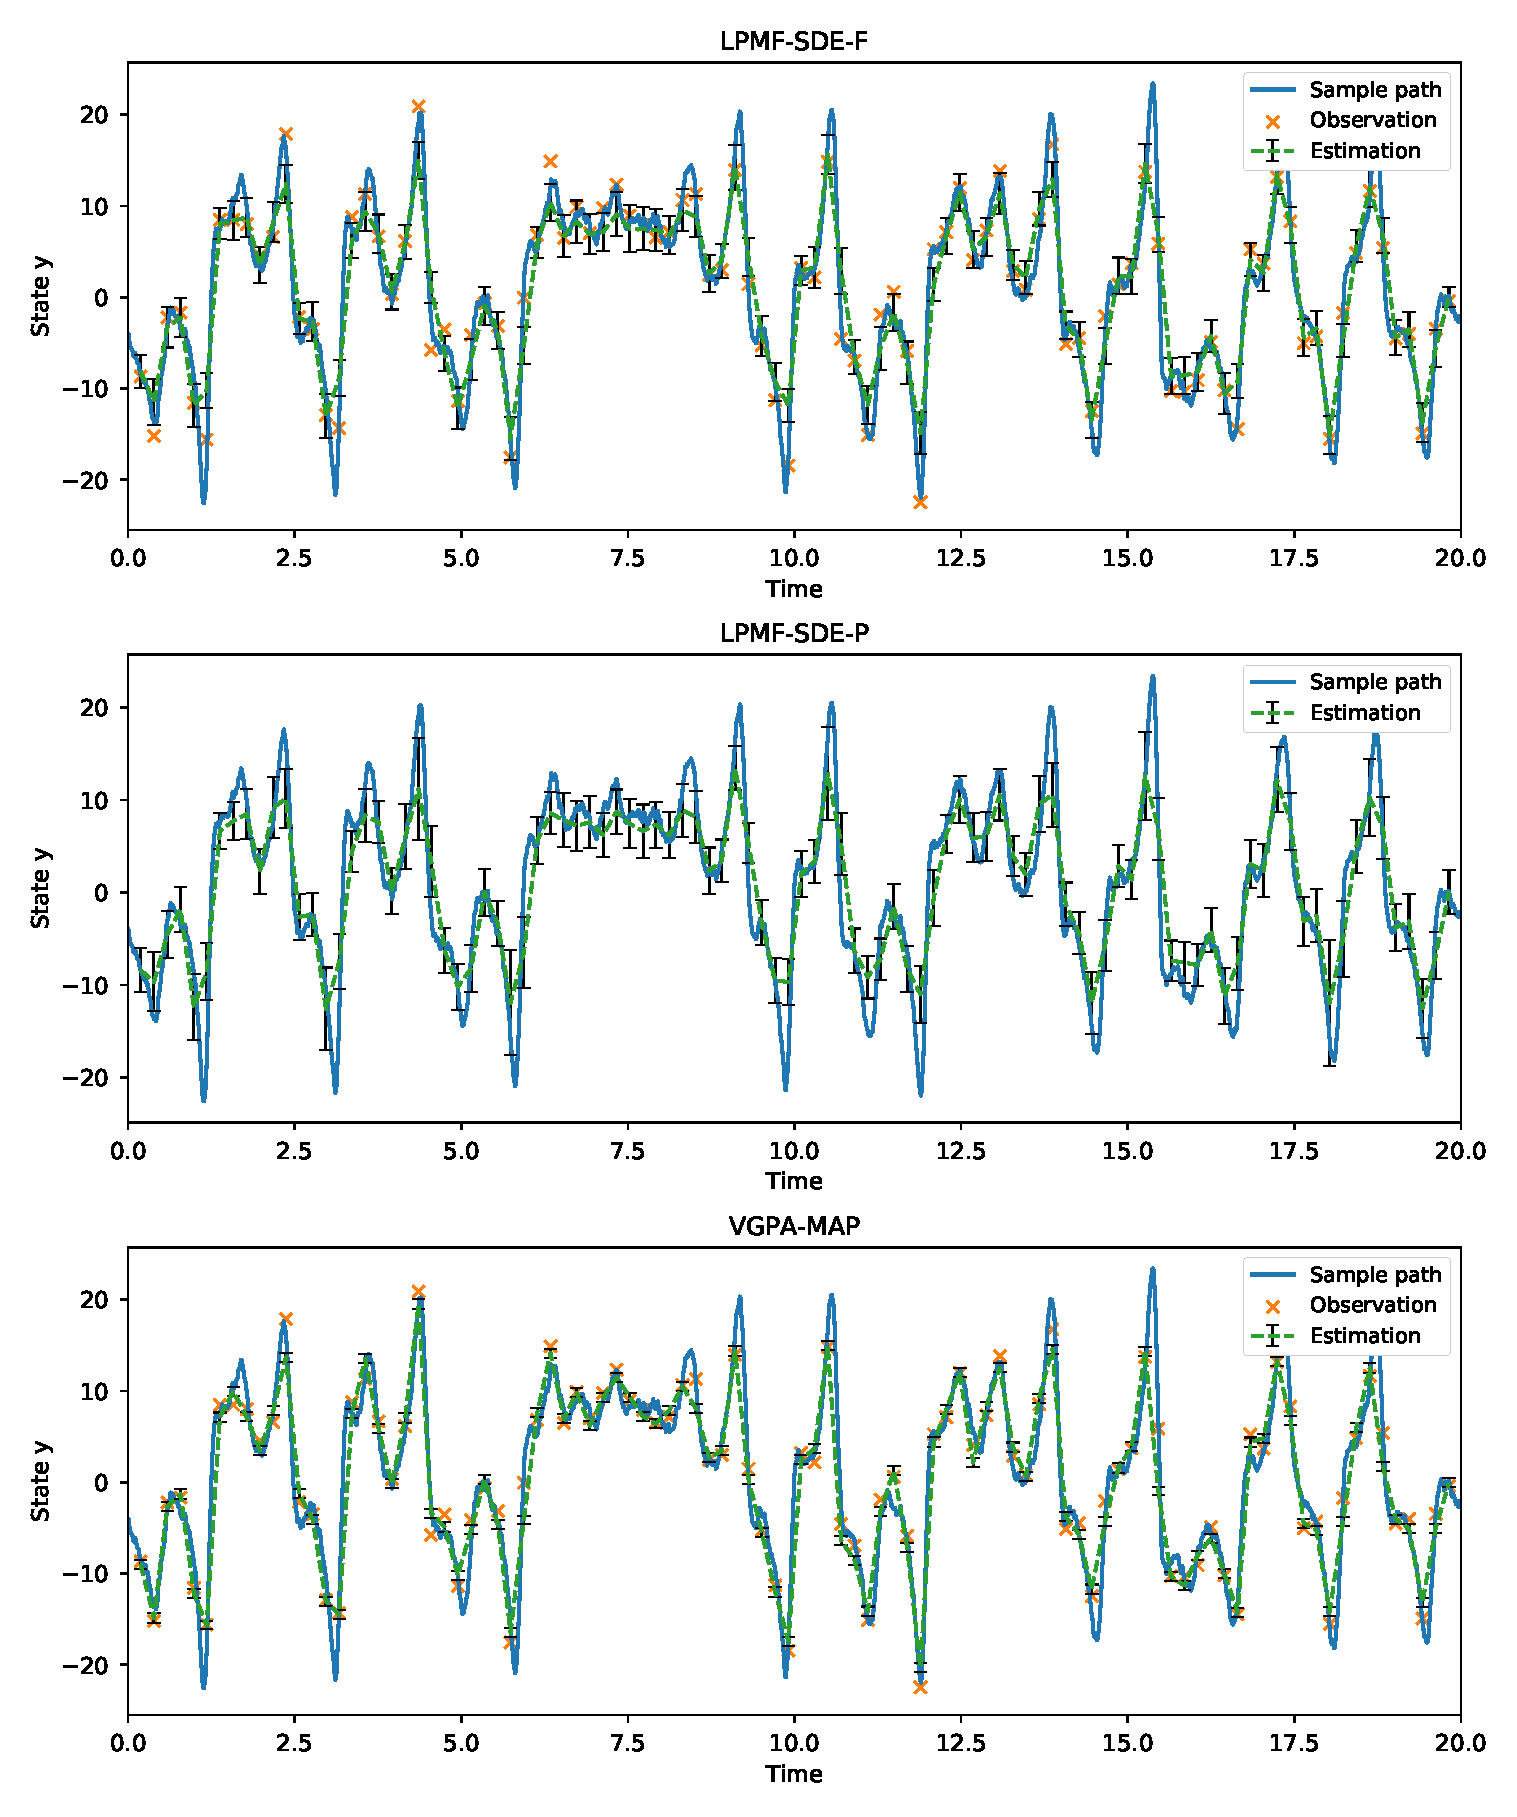
\includegraphics[width=\textwidth]{graphics/lorenz-63-states}
    \caption{Estimation for state $y$ of the stochastic Lorenz 63 model. The top and middle plots are the results for the fully and partially observable cases using the \algolpmfsde\ method respectively. The bottom plot contains the result for the fully observable case using the \algovgpamap\ extension. The ground truth is shown as a solid blue line. The mean of the estimation is drawn as a dotted green line together with the error bars indicating one standard deviation. Observations, when available, are indicated by the orange crosses.}
    \label{fig-lorenz-63-states}
\end{figure}

\begin{figure}
    \centering
    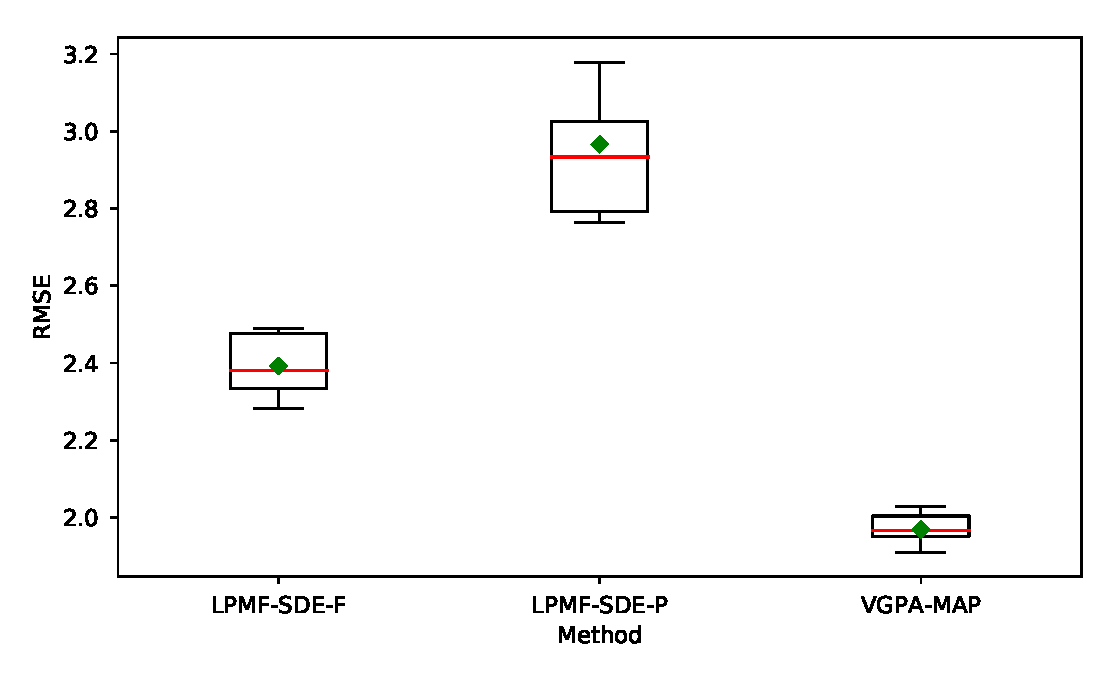
\includegraphics[width=0.8\linewidth]{graphics/lorenz-63-states-boxplot}
    \caption{Box plot for the RMSEs of state estimation over 10 independent SDE sample paths from the stochastic Lorenz 63 model. In the box plot, the median is indicated by the red line, while the mean is shown as the green diamond. The box shows the lower and upper quartiles, while the whiskers are the 5th and 95th percentiles.}
    \label{fig-lorenz-63-state-boxplot}
\end{figure}

The estimation for state $y$ from one SDE sample path is shown in \reffigure{\ref{fig-lorenz-63-states}}.
Similar to the result for the stochastic Lorenz 96 model in \refsection{\ref{sec-lorenz-96}}, the general trend of the state is sucessfully captured by both methods with minor differences on the details.
The \algovgpamap\ method seem to be better at points where the state changes dramatically to form high and low peaks.
The variance of the estimation is also lower than the \algolpmfsde\ approach.
One the other hand, it is worth noting that the \algolpmfsde\ method even functions quite well when state $y$ is unobserved but with naturally higher uncertainty, especially around the peaks.
Since state $y$ is unobserved, the only source of information to estimate it is from the drift function \refequationp{\ref{eq-lorenz-63-odes}}, which is demonstrates the potential of the gradient matching framework.

After repeating the above experiment 10 times using each time an independently generated SDE sample path and observation set, the RMSEs for state estimation is computed and summarized in \reffigure{\ref{fig-lorenz-63-state-boxplot}}.
Since there are only three states, the RMSEs over all states are considered together.
The figure shows that the RMSE of state estimation using \algovgpamap\ is slightly below the observation noise variance, which outperforms \algolpmfsde\ with full state observability by around 0.4 on average.
On the other hand, the RMSE using \algolpmfsde\ when state $y$ is unobserved is still reasonably low, considering that the values of the state range from -20 to 20, and the inference is carried out over a much longer time period than all previous experiments.

\subsubsection*{Parameter estimation}

\begin{figure}
    \centering
    \begin{subfigure}{0.48\textwidth}
        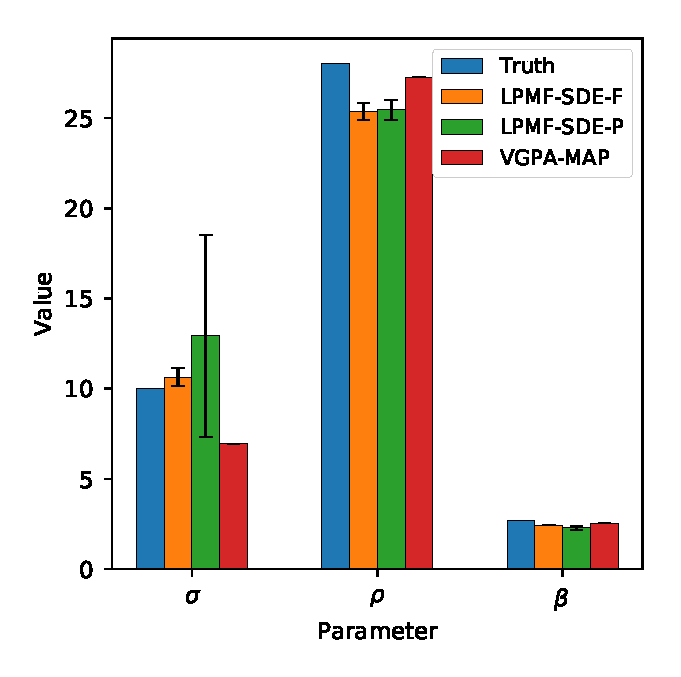
\includegraphics[width=\linewidth]{graphics/lorenz-63-parameters}
        \caption{\ }
        \label{fig-lorenz-63-parameters}
    \end{subfigure}
    \begin{subfigure}{0.48\textwidth}
        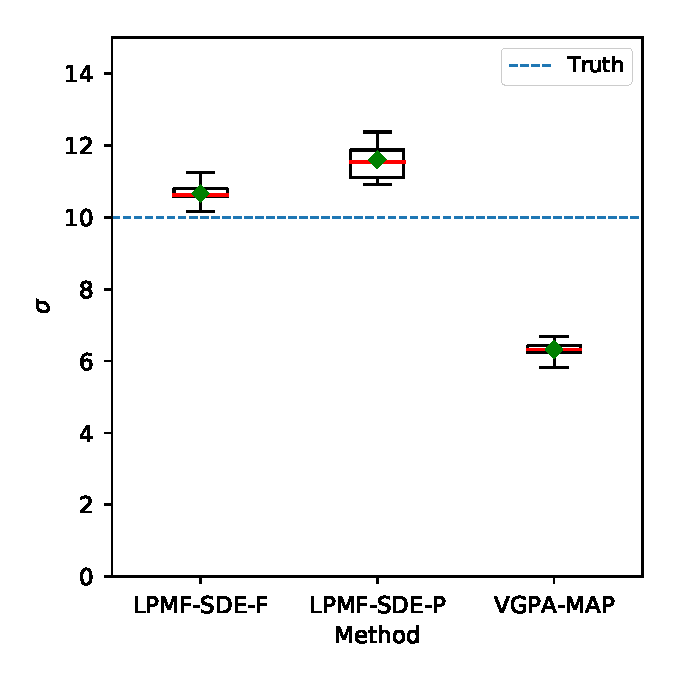
\includegraphics[width=\linewidth]{graphics/lorenz-63-parameters-sigma-boxplot}
        \caption{\ }
        \label{fig-lorenz-63-parameters-sigma-boxplot}
    \end{subfigure}
    \begin{subfigure}{0.48\textwidth}
        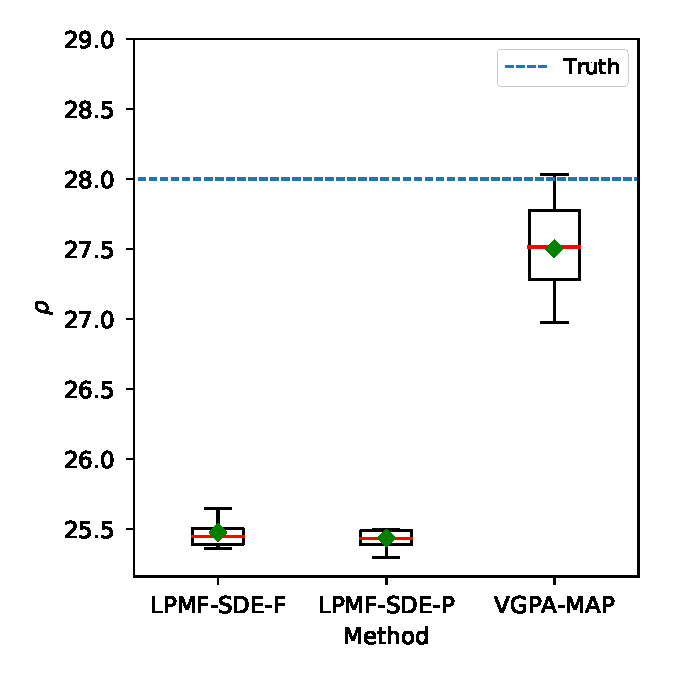
\includegraphics[width=\linewidth]{graphics/lorenz-63-parameters-rho-boxplot}
        \caption{\ }
        \label{fig-lorenz-63-parameters-rho-boxplot}
    \end{subfigure}
    \begin{subfigure}{0.48\textwidth}
        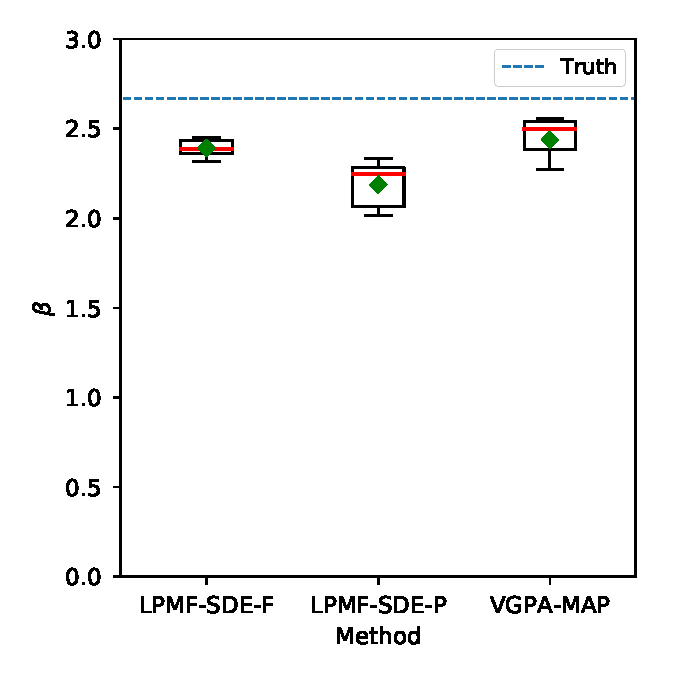
\includegraphics[width=\linewidth]{graphics/lorenz-63-parameters-beta-boxplot}
        \caption{\ }
        \label{fig-lorenz-63-parameters-beta-boxplot}
    \end{subfigure}
    \caption{Parameter estimation result for the stochastic Lorenz 63 model. (a) Estimation result for the SDE sample path shown in \reffigure{\ref{fig-lorenz-63-states}} with the error bar indicating one standard deviation. (b), (c), and (d) are the box plots for parameters $\sigma$,  $\rho$ and $\beta$ after 10 independent repetitions respectively. In the box plot, the median is indicated by the red line, while the mean is shown as the green diamond. The box shows the lower and upper quartiles, while the whiskers are the 5th and 95th percentiles. The dotted blue line indicates the true parameter value.}
    \label{fig-lorenz-63-parameters-group}
\end{figure}

For parameter estimation, the results are presented in \reffigure{\ref{fig-lorenz-63-parameters-group}}.
Overall, the estimation based on both methods seem to be on par with each other with relatively low variance when all the states are observed.
Given that the \algovgpamap\ algorithm achieves better accuracy when estimating the states, it would be expected that the parameter estimation to also be better.
The non-optimal performance is probably due to the simple gradient update strategy as mentioned before.

If we look at \reffigure{\ref{fig-lorenz-63-parameters}} in detail, the large variance around the estimation for parameter $\sigma$ when state $y$ is unobserved is noticeable.
To explain this, first note that $\sigma$ appears only inside the first equation of \refequationp{\ref{eq-lorenz-63-odes}} together with state $x$ and $y$.
Since $y$ is not observable, the only source of information to estimate $\sigma$ is  $x$.
This is in contrast to the other two parameters $\rho$ and $\beta$, where both states $x$ and $z$ are used to estimate them.
Lastly, the means of the predicted parameters over the 10 independent runs are generally concentrated except for parameter $\rho$ inferred by the \algovgpamap\ algorithm, as shown in \reffigure{\ref{fig-lorenz-63-parameters-sigma-boxplot}} to \reffigure{\ref{fig-lorenz-63-parameters-rho-boxplot}}.

\subsubsection*{Runtime performance}

\begin{figure}
    \centering
    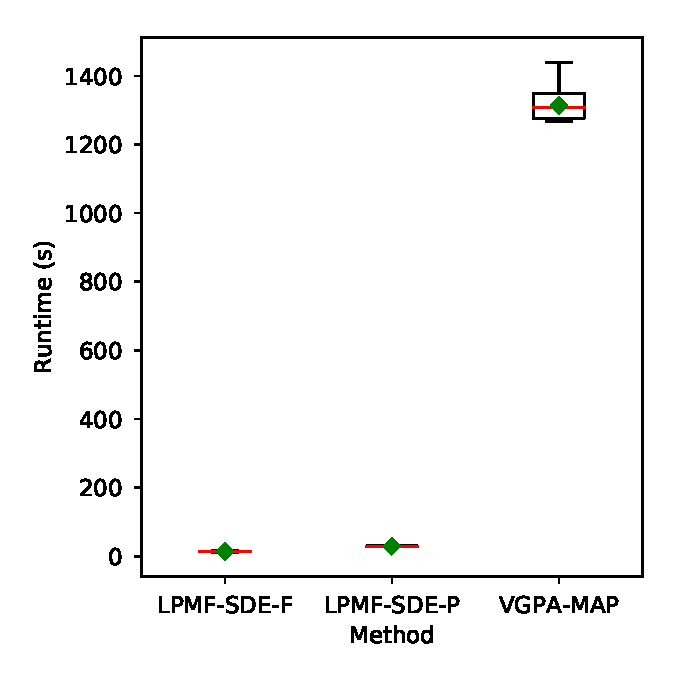
\includegraphics[width=0.48\linewidth]{graphics/lorenz-63-runtime-boxplot}
    \caption{Box plot for the runtimes over 10 repetitions using independent sample paths from the stochastic Lorenz 63 model. The median is indicated by the red line, while the mean is shown as the green diamond. The box shows the lower and upper quartiles, while the whiskers are the 5th and 95th percentiles.}
    \label{fig-lorenz-63-runtime-boxplot}    
\end{figure}

\reffigure{\ref{fig-lorenz-63-runtime-boxplot}} shows the distribution of the average time to solve one RODE sample path and the runtime of the \algovgpamap\ algorithm to infer one SDE sample path after 10 independent repetitions. 
For each RODE sample, \algolpmfsde\ takes a fraction of the time required by \algovgpamap\ for one SDE sample path.
Even if the RODEs are not solved in parallel, the total runtime required by \algolpmfsde\ is still comparable to that of \algovgpamap. 
This further demonstrates the runtime efficiency of the \algolpmfsde\ scheme.


\chapter{Conclusion}
\label{ch-conclusion}

This work examines the problem of state and parameter estimation in deterministic and random dynamical systems given noisy, sparse or even incomplete observations.
A mean-field Laplace approximation solution is proposed to address the intractability of the posterior distribution and has been shown empirically to be robust and scalable.
Further, it relaxes the structural assumption imposed on the dynamical systems from previous work and introduces positivity constraints on the states and parameters.
Based on the correspondence between RODEs and SDEs, a highly efficient parallel inference technique is devised to address problems involving diffusion processes.


%\appendix

%\input{appendix}

\backmatter

\nocite{*}

\bibliographystyle{abbrvnat-updated}
\bibliography{refs}

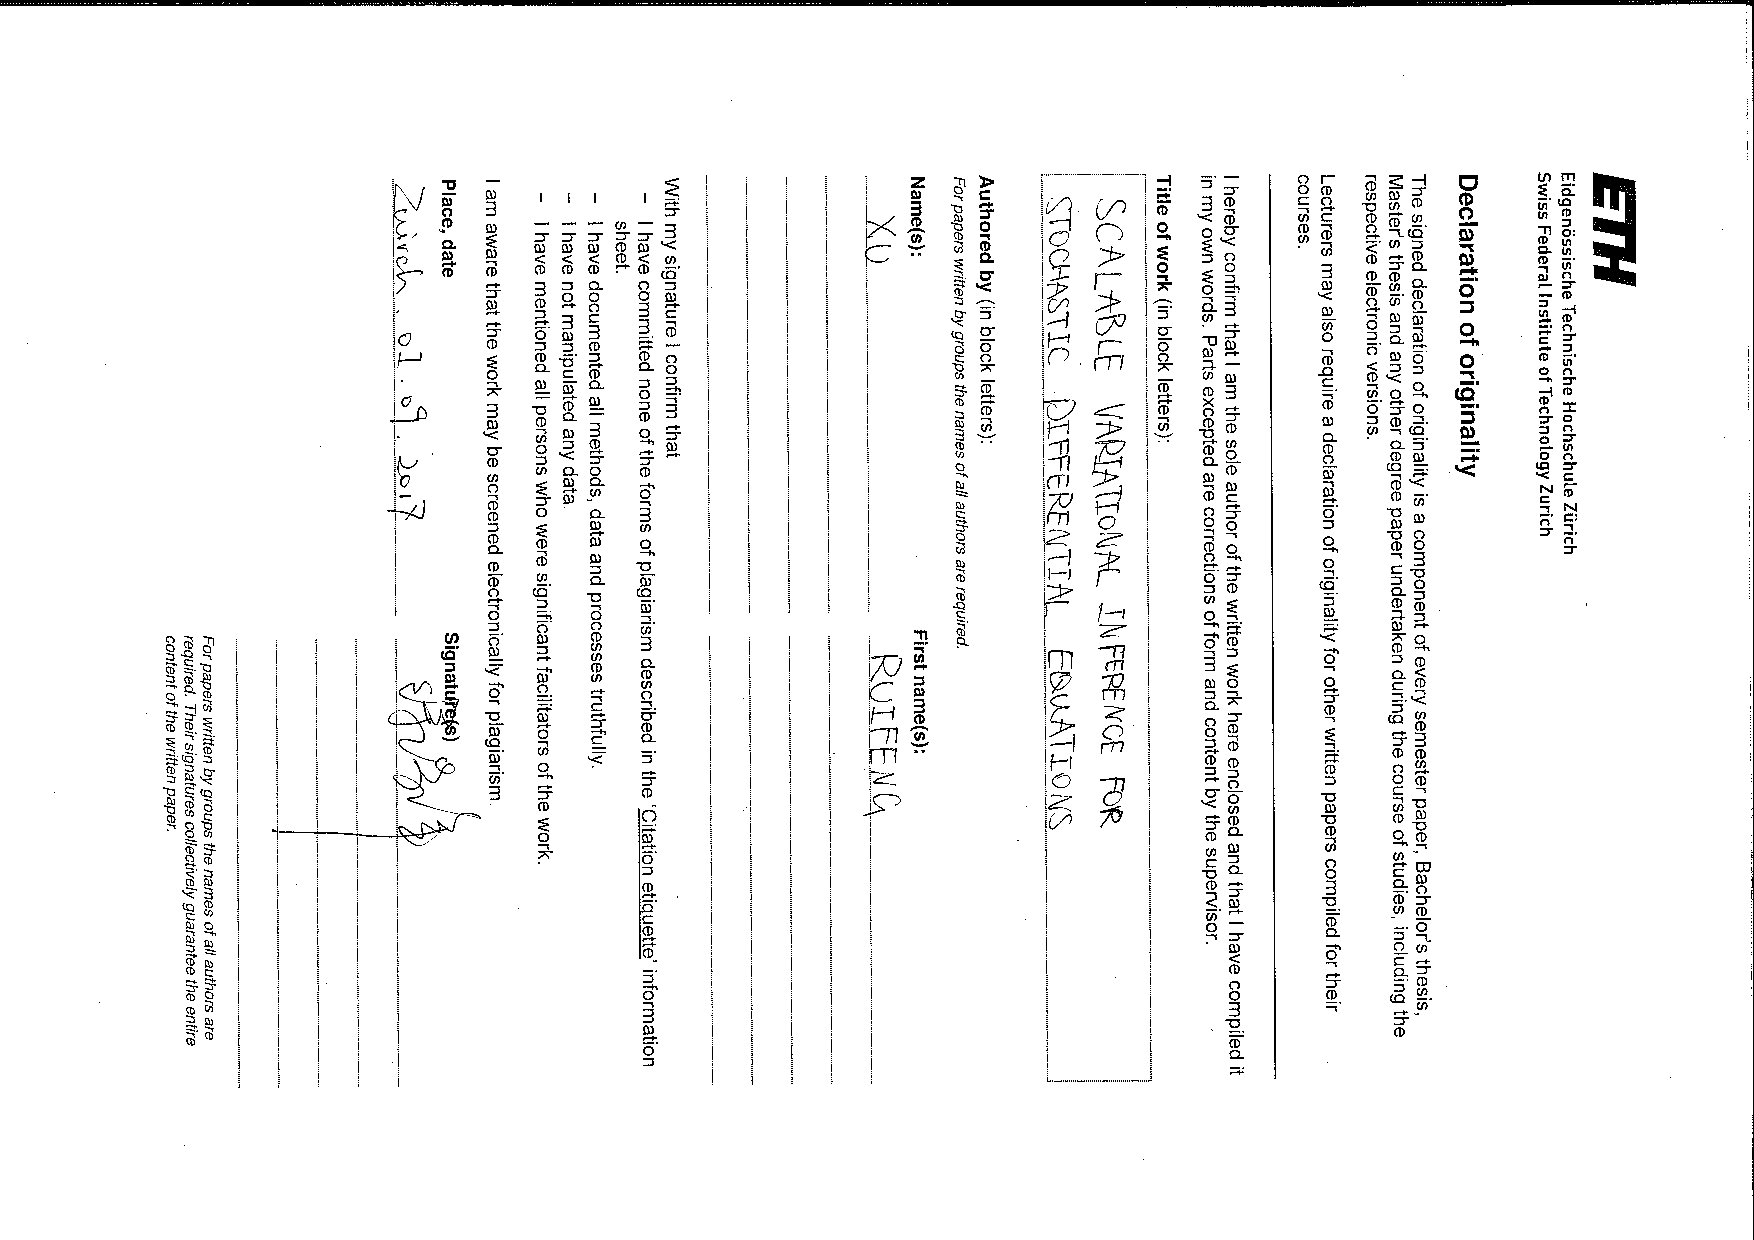
\includepdf[pages={-}]{declaration-originality.pdf}

\end{document}
